% Options for packages loaded elsewhere
\PassOptionsToPackage{unicode}{hyperref}
\PassOptionsToPackage{hyphens}{url}
%
\documentclass[
]{article}
\usepackage{amsmath,amssymb}
\usepackage{lmodern}
\usepackage{iftex}
\ifPDFTeX
  \usepackage[T1]{fontenc}
  \usepackage[utf8]{inputenc}
  \usepackage{textcomp} % provide euro and other symbols
\else % if luatex or xetex
  \usepackage{unicode-math}
  \defaultfontfeatures{Scale=MatchLowercase}
  \defaultfontfeatures[\rmfamily]{Ligatures=TeX,Scale=1}
\fi
% Use upquote if available, for straight quotes in verbatim environments
\IfFileExists{upquote.sty}{\usepackage{upquote}}{}
\IfFileExists{microtype.sty}{% use microtype if available
  \usepackage[]{microtype}
  \UseMicrotypeSet[protrusion]{basicmath} % disable protrusion for tt fonts
}{}
\makeatletter
\@ifundefined{KOMAClassName}{% if non-KOMA class
  \IfFileExists{parskip.sty}{%
    \usepackage{parskip}
  }{% else
    \setlength{\parindent}{0pt}
    \setlength{\parskip}{6pt plus 2pt minus 1pt}}
}{% if KOMA class
  \KOMAoptions{parskip=half}}
\makeatother
\usepackage{xcolor}
\usepackage[margin=1.0in]{geometry}
\usepackage{graphicx}
\makeatletter
\def\maxwidth{\ifdim\Gin@nat@width>\linewidth\linewidth\else\Gin@nat@width\fi}
\def\maxheight{\ifdim\Gin@nat@height>\textheight\textheight\else\Gin@nat@height\fi}
\makeatother
% Scale images if necessary, so that they will not overflow the page
% margins by default, and it is still possible to overwrite the defaults
% using explicit options in \includegraphics[width, height, ...]{}
\setkeys{Gin}{width=\maxwidth,height=\maxheight,keepaspectratio}
% Set default figure placement to htbp
\makeatletter
\def\fps@figure{htbp}
\makeatother
\setlength{\emergencystretch}{3em} % prevent overfull lines
\providecommand{\tightlist}{%
  \setlength{\itemsep}{0pt}\setlength{\parskip}{0pt}}
\setcounter{secnumdepth}{-\maxdimen} % remove section numbering
\newlength{\cslhangindent}
\setlength{\cslhangindent}{1.5em}
\newlength{\csllabelwidth}
\setlength{\csllabelwidth}{3em}
\newlength{\cslentryspacingunit} % times entry-spacing
\setlength{\cslentryspacingunit}{\parskip}
\newenvironment{CSLReferences}[2] % #1 hanging-ident, #2 entry spacing
 {% don't indent paragraphs
  \setlength{\parindent}{0pt}
  % turn on hanging indent if param 1 is 1
  \ifodd #1
  \let\oldpar\par
  \def\par{\hangindent=\cslhangindent\oldpar}
  \fi
  % set entry spacing
  \setlength{\parskip}{#2\cslentryspacingunit}
 }%
 {}
\usepackage{calc}
\newcommand{\CSLBlock}[1]{#1\hfill\break}
\newcommand{\CSLLeftMargin}[1]{\parbox[t]{\csllabelwidth}{#1}}
\newcommand{\CSLRightInline}[1]{\parbox[t]{\linewidth - \csllabelwidth}{#1}\break}
\newcommand{\CSLIndent}[1]{\hspace{\cslhangindent}#1}
\usepackage{upgreek}
\usepackage{booktabs}
\usepackage{longtable}
\usepackage{graphicx}
\usepackage{array}
\usepackage{multirow}
\usepackage{wrapfig}
\usepackage{float}
\usepackage{colortbl}
\usepackage{pdflscape}
\usepackage{tabu}
\usepackage{threeparttable}
\usepackage{threeparttablex}
\usepackage[normalem]{ulem}
\usepackage{makecell}
\usepackage{setspace}
\doublespacing
\usepackage[left]{lineno}
\linenumbers
\modulolinenumbers
\usepackage{helvet} % Helvetica font
\renewcommand*\familydefault{\sfdefault} % Use the sans serif version of the font
\usepackage[T1]{fontenc}
\usepackage[shortcuts]{extdash}
\usepackage[document]{ragged2e}
\ifLuaTeX
  \usepackage{selnolig}  % disable illegal ligatures
\fi
\IfFileExists{bookmark.sty}{\usepackage{bookmark}}{\usepackage{hyperref}}
\IfFileExists{xurl.sty}{\usepackage{xurl}}{} % add URL line breaks if available
\urlstyle{same} % disable monospaced font for URLs
\hypersetup{
  hidelinks,
  pdfcreator={LaTeX via pandoc}}

\author{}
\date{\vspace{-2.5em}}

\begin{document}

\raggedright

\hypertarget{waste-not-want-not-revisiting-the-analysis-that-called-into-question-the-practice-of-rarefaction}{%
\section{Waste not, want not: Revisiting the analysis that called into
question the practice of
rarefaction}\label{waste-not-want-not-revisiting-the-analysis-that-called-into-question-the-practice-of-rarefaction}}

\vspace{20mm}

\textbf{Running title:} Revisiting ``Waste not, want not''

\vspace{20mm}

Patrick D. Schloss\({^\dagger}\)

\vspace{40mm}

\({\dagger}\) To whom corresponsdence should be addressed:

\href{mailto:pschloss@umich.edu}{pschloss@umich.edu}

Department of Microbiology \& Immunology

University of Michigan

Ann Arbor, MI 48109

\vspace{20mm}

\textbf{Research article}

\newpage

\hypertarget{abstract}{%
\subsection{Abstract}\label{abstract}}

\newpage

\hypertarget{introduction}{%
\subsection{Introduction}\label{introduction}}

Microbiome studies that use amplicon sequencing to characterize multiple
samples use PCR to amplify 16S rRNA gene fragments using primers with
distinct barcodes or index sequences {[}(1); \textbf{XXXXX}{]}. These
barcodes allow researchers to pool PCR products and then deconvolute the
resulting sequence data based on the barcode sequences. Despite their
best efforts to generate equimolar pools of PCR products, it is common
to observe more than 10-fold variation in the number of sequences per
sample {[}\textbf{XXXXX}{]}. Researchers desire strategies to minimize
uneven sequencing depth and thus need methods to control for this
uneveness in their analyses. Of course, uneven sampling is not unique to
microbiome research and is a challenge faced by all community ecologists
{[}\textbf{XXXXX}{]}. Common approaches to controlling uneven sampling
efforts include use of proportional abundance (i.e., relative
abundance), scaling of counts, parameter estimation, and rarefaction
{[}\textbf{XXXXX}{]}.

In 2014 Paul McMurdie and Susan Holmes published ``Waste not, want not:
why rarefying microbiome data is inadmissible'' (WNWN) in \emph{PLOS
Computational Biology} (2). Their paper has had a significant impact on
the approaches that microbiome researchers use to analyze 16S rRNA gene
sequence data. According to Google Scholar, this paper has been cited
more than 2,400 times as of June 2023. There has been a rebuttal of WNWN
that actually showed how rarefaction could be beneficial (3).
Anecdotely, I have received correspondence from researchers over the
past 10 years asking how to address critiques from reviewers who
criticize my correspondents' analysis for using rarefaction (e.g., see
\href{https://twitter.com/inanna_nalytica/status/1264299305067786242}{this
Twitter thread}). I have also received similar comments from reviewers
regarding my own work. Most recently, I received the critique for a
preprint that I posted in 2020 that analyzed the practice of removing
rare taxa from microbiome analyses {[}see comments linked to
\textbf{XXXXX};
\url{https://web.archive.org/web/20230308191505/http://dalmug.org/filter-review/}{]}.
In the process of responding to these reviewers' comments and preparing
a manuscript investigating rarefaction and other approaches to control
for uneven sequencing effort, I grew to appreaciate that there is
signifcant confusion in the field over what is meant by ``rarefying''
and ``rarefaction''.

McMurdie and Holmes discussed and defined ``rarefying'' in WNWN
(citation numbers updated from the original to those of the current
study):

\begin{quote}
``Instead, microbiome analysis workflows often begin with an ad hoc
library size normalization by random subsampling without replacement, or
so-called rarefying (4--6). There is confusion in the literature
regarding terminology, and sometimes this normalization approach is
conflated with a non-parametric resampling technique --- called
rarefaction (7), or individual-based taxon re-sampling curves (8) ---
that can be justified for coverage analysis or species richness
estimation in some settings (8), though in other settings it can perform
worse than parametric methods (9). Here we emphasize the distinction
between taxon re-sampling curves and normalization by strictly adhering
to the terms rarefying or rarefied counts when referring to the
normalization procedure, respecting the original definition for
rarefaction. Rarefying is most often defined by the following steps (5).

\begin{enumerate}
\def\labelenumi{\arabic{enumi}.}
\tightlist
\item
  Select a minimum library size, N\textsubscript{L,m}. This has also
  been called the rarefaction level (4), though we will not use the term
  here.
\item
  Discard libraries (microbiome samples) that have fewer reads than
  N\textsubscript{L,m}.
\item
  Subsample the remaining libraries without replacement such that they
  all have size N\textsubscript{L,m}.
\end{enumerate}

Often N\textsubscript{L,m} is chosen to be equal to the size of the
smallest library that is not considered defective, and the process of
identifying defective samples comes with a risk of subjectivity and
bias. In many cases researchers have also failed to repeat the random
subsampling step (3) or record the pseudorandom number generation
seed/process --- both of which are essential for reproducibility.''
\end{quote}

It was unfortunate that McMurdie and Holmes used the term ``rarefying''
here and throughout their manuscript. The authors were correct to state
that the distinction between ``rarefying'' and ``rarefaction'' is
confusing and leads to their conflation. Adding to the confusion is that
the papers cited in the first sentence of this quote (i.e., (4--6))
either do not use the words ``rarefy'' or ``rarefying'' or use them
interchangably with ``rarefaction''. For example, Hughes and Hellman did
not use ``rarefy'' and use ``rarefaction'' in the traditional sense with
multiple subsamplings (5). Meanwhile, the QIIME-based literature appears
to use ``rarefy'' and ``rarefaction'' interchangibly meaning only a
single subsampling ((4, 6)). Subsequent researchers have continued to
conflate the results of this study of the effects of rarefying data with
that of traditional rarefaction of data (\textbf{Supplemental Text}). An
exemplar of the confusion is the creation of a technique that uses
``repeatedly rarefying'' as an approach distinct from rarefaction when
they are actually the same thing (10).

As shown in the quoted text from WNWN, McMurdie and Holmes did emphasize
the distinction between rarefying and rarefaction. However, because they
seem to have coined a new definition for rarefying, they added to the
confusion by using the generally used verb form of rarefaction. Further
confusion comes from the author's admonition in the final sentence of
the above quoted text that some researchers have failed to repeat the
subsampling step. Classically, repeating the subsampling step is
rarefaction {[}\textbf{XXXXX}{]}. In other words, subsampling is
rarefaction, but with a single randomization. To minimize confusion, I
will use ``subsamping'' in place of ``rarefying'' thorugh the remainder
of this study.

For clarity, I will use the following definition of rarefaction:

\begin{enumerate}
\def\labelenumi{\arabic{enumi}.}
\tightlist
\item
  Select a minimum library size, N\textsubscript{L,m}. Researchers are
  encouraged to report the value of N\textsubscript{L,m}.
\item
  Discard samples that have fewer reads than N\textsubscript{L,m}.
\item
  Subsample the remaining libraries without replacement such that they
  all have size N\textsubscript{L,m}.
\item
  Compute the desired metric (e.g., richness, Shannon diversity,
  Bray-Curtis distances) using the subsampled data
\item
  Repeat steps 3 and 4 a large number of iterations (e.g, 100 or 1,000).
  Researchers are encouraged to report the number of iterations.
\item
  Compute summary statistics (e.g., the mean) using the values from step
  4.
\end{enumerate}

This definition aligns with how rarefaction was originally defined for
comparing richness (i.e., the number of taxa in a community) across
communities when communities are sampled to different depths
{[}\textbf{XXXXX}{]}. With this more general approach to the definition
of rarefaction, rarefaction can be performed using any alpha or beta
diversity metric. This strategy has been widely used by my research
group and others and is available in the mothur software package using
commands such as \texttt{summary.single}, \texttt{rarefaction.single},
\texttt{phylo.diversity}, and \texttt{dist.shared}. The procedure
outlined above could also be used for hypothesis tests of differential
abundance; however, consideration is needed to synthesize the results of
these tests across a large number of replications.

\hypertarget{description-and-critique-of-simulation-a-from-wnwn}{%
\subsection{Description and critique of ``Simulation A'' from
WNWN}\label{description-and-critique-of-simulation-a-from-wnwn}}

McMurdie and Holmes analyzed the effect of subsampling and other
approaches on clustering accuracy using what they called ``Simulation
A'' in their Figure 2A and elsewhere in their paper. In Simulation A,
they investigated the ability to correctly assign simulated microbiome
samples to one of two clusters representing two simulated treatment
groups. Thankfully, the R code for Simulation A was provided by the
authors in the
\texttt{simulation-cluster-accuracy/simulation-cluster-accuracy-server.Rmd}
R-flavored markdown file that was published as Protocol S1 in WNWN. I
will outline the simulation strategy below and will reference line
numbers from their R-flavored markdown file with ``L'' as a prefix.

For the WNWN cluster analysis, sampling distributions for the two
treatment groups were generated using human fecal and ocean data
originally take from the GlobalPaterns dataset (L129) (1). To generate a
fecal and ocean distribution, the authors included any operational
taxonomic unit (OTU) that appeared in more than one of the 4 fecal and 3
ocean samples (L60 and L137). The OTUs were sorted by how many of the 7
samples the OTUs were observed in followed by their total abundance
across all 7 samples (L139). From this sorted list they identified the
identifiers of the first 2,000 OTUs (L66). Returning to the 7 samples
they selected the data for the corresponding 2,000 OTUs and pooled the
OTU abundances of the fecal and ocean samples separately to create two
sampling distributions (L144, L159-160, L197-198). Next, the fecal and
ocean distributions were mixed in 8 different fractions to generate two
community types that differend by varying effect sizes (i.e., 1.0, 1.15,
1.25, 1.5, 1.75, 2, 2.5, and 3.5; L170-195, L220); an effect size of 1.0
generated a null model with no difference between the treatment groups.
To simulate the variation in sequencing depth across the 80 samples,
they normalized the number of sequences from each of the 26 samples in
the GlobalPatterns dataset so that the median number of sequences
(Ñ\textsubscript{L}) across the samples had 1,000, 2,000, 5,000, or
10,000 sequences (L324-325). They then randomly sampled the 26
normalized sequencing depths, with replacement, to generate 80 sampling
depths. From each community type, they simulated 40 samples by sampling
to the desired number of sequences (L73, L230-233 and L326-327). Each
simulation condition was repeated 5 times (L85). Finally, they removed
rare and low prevalence OTUs in two steps. First, they removed any OTUs
whose total abundance was less than 3 across all 80 samples and that did
not appear in at least 3 samples (L368-386). Second, they removed any
OTUs that did not have more than 1 sequence in more than 5\% of the 80
samples (i.e., 4 samples) and that did not have a total abundance across
the 80 samples greater than one half of the number of samples in each
community type (i.e., 20) (L523-538, L551). Simulation A consisted of
160 simulations (8 effect sizes x 4 median sampling depths x 5
replicates = 160 simulations).

After generating the OTU counts for the 160 simulations, the authors
applied several normalization methods, distance calculations, and
clustering algorithms to the data. To normalize the OTU data the WNWN
analysis either applied no normalization procedure (L559), calculated
OTU relative abundances (L392-401, L562-563), subsampled the data
(L409-416, L566-569), performed variance stabilization using the DESeq R
package (L478-504, L580-583), or performed Upper-Quartile log-fold
change normalization using the edgeR R package (L425-457, L576-577,
L622-721). In subsampling the data, the authors either included all of
the samples or removed samples whose sequencing depth fell below the 5,
10, 15, 20, 25, and 40 percentile across all 80 samples (L96,
L1065-1077). Non-normalized data were used to calculate Bray-Curtis,
Euclidean, Poisson, and Weighted UniFrac distances (L793-798, L801-806).
Relative abundance data were used to calculate Bray-Curtis, Unweigthed
UniFrac, and Weighted UniFrac distances (L760-767). Subsampled data were
then used as input to calculate distances between samples using
Bray-Curtis, Euclidean, Unweighted UniFrac, and Weighted Unifrac
distances as implemented in the Phyloseq R package, Poisson distances as
implemented in the PoiClaClu R package, and top-mean squared difference
as implemented in the edgeR R package (L769-775, L793-798, L801-806).
DESeq variance stabilization normalized data were used to calculate
Bray-Curtis, Euclidean, and Weighted Unifrac distances (L793-798). The
Upper-Quartile log-fold change normalized data were only used to
calculate top-mean squared difference distances (L801-806). The
resulting distance matrices were used to cluster the 80 samples into one
of two clusters using partitioning around the medoid (PAM), K-means
clustering, and hierarchical clustering (L865-879). Although data for
all three methods were presented in the supplementary Protocol S1, only
the PAM data are presented in the main manuscript. The accuracy of the
clustering assignments was quantified as the fraction of the 80 samples
that were assigned to the correct cluster (L887-908). Since some of the
subsampling conditions removed samples below a minimum sequencing depth
threshold, those samples were counted as mis-clustered samples yielding
minimum accuracies below 50\%.

Although all simulations represent an artificial representation of
reality and can be critiqued, eleven elements of the design of
Simulation A warrant further review.

\begin{enumerate}
\def\labelenumi{\arabic{enumi}.}
\tightlist
\item
  Simulated conditions were only replicated 5 times each, potentially
  increasing the sensitivity of results to the choice of the random
  number generator seed
\item
  The average sizes of the libraries were small by modern standards,
  which may limit the generalizability of the results
\item
  DESeq-based variance stabilization was used with distance calculation
  methods that are sensitive to negative values, which likely led to
  nonsense distances and clusters
\item
  A single subsampling of each dataset was evaluated rather than using
  rarefaction, which likely resulted in noisier data
\item
  Results using PAM clustering were not directly compared to those of
  K-means and hierarchical clustering, although close inspection
  suggests that K-means may have been superior to PAM for some
  conditions
\item
  Subsampling removed the smallest 15\% of the samples, which penalized
  accuracy values by 15 percentage points
\item
  The distribution of library sizes was not typical of those commonly
  seen in microbiome analyses, which may limit the generalizability of
  the results
\item
  A filtering step was applied to remove rare taxa from the simulated
  datasets, which may have skewed the shape of the community
  distributions
\item
  There was no accounting for differences in performance when library
  sizes are confounded with treatment group
\item
  Clustering accuracy was used rather than the more direct and
  frequently applied comparisons of beta diversity using permutation
  tests
\item
  There was no consideration of effects of normalization methods on
  alpha diversity metrics, which is the traditional application of
  rarefaction
\end{enumerate}

After replicating the original WNWN simulations, these points will be
evaluated to reassess whether subsampling or rarefaction are
``inadmissible''.

\hypertarget{results}{%
\subsection{Results}\label{results}}

\hypertarget{replication-of-wnwn-simulations-and-results}{%
\subsubsection{Replication of WNWN simulations and
results}\label{replication-of-wnwn-simulations-and-results}}

Before assessing the impact of the points I critiqued above, I attempted
to replicate the results shown in Figures 4 and 5 of WNWN using the
authors' code. I created a Conda environment that used the R version and
package versions that were as close as possible to those used in WNWN.
It was necessary to patch the WNWN's R-flavored markdown file to render
the document to be compatible with the overall workflow of this study. I
was able to generate figures similar to those presented as WNWN's
Figures 4 and 5; my results are shown in this study as Figures 1 and 2,
respectively. The differences in results are likely due to differences
in software versions and operating systems. It is also worth noting that
the published versions of the two figures differ from those included in
Protocol S1 within the rendered HTML file
(\texttt{simulation-cluster-accuracy/simulation-cluster-accuracy-server.html})
and that the figure numbers are one higher in the paper than those
generated by the R-flavored markdown file (i.e., Protocol S1 labels the
figures as Figures 3 and 4 corresponding to the published Figures 4 and
5). Regardless of the differences, my results were qualitatively similar
to that provided in WNWN's Protocol S1.

\hypertarget{simulated-conditions-were-only-replicated-5-times-each-potentially-increasing-the-sensitivity-of-results-to-the-choice-of-the-random-number-generator-seed}{%
\subsubsection{1. Simulated conditions were only replicated 5 times
each, potentially increasing the sensitivity of results to the choice of
the random number generator
seed}\label{simulated-conditions-were-only-replicated-5-times-each-potentially-increasing-the-sensitivity-of-results-to-the-choice-of-the-random-number-generator-seed}}

Each simulated condition was replicated 5 times in WNWN and the paper
reports the mean and standard deviation of the replicate clustering
accuracies. The relatively small number of replicates accounts for the
jerkiness of the lines in WNWN's Figures 4 and 5 (e.g.~the Bray-Curtis
distances calculated on the DESeqVS normalized data). A better approach
would have been to use 100 replicates as this would reduce the
dependency of the results on the random number generator's seed. By
increasing the number of replicates it was also possible to compare the
probability of falsely and correctly clustering samples from the same
and different treatment groups together (see points 9-11, below).
Because the accuracies were not symmetric around the mean accuracy
values the median and 95\% confidence intervals or intraquartile range
should have been reported. To test the effect of increasing the number
of replicates, I pulled apart the code in
\texttt{simulation-cluster-accuracy/simulation-cluster-accuracy-server.Rmd}
into individual R and bash scripts that were executed using a Snakemake
workflow with the same Conda environment I used above. This was
necessary since the number of simulated conditions increased 20-fold
with the additional replicates. Such intense data processing was not
practical within a single R-flavored markdown document. Again, the
observed results were qualitiatively similar to those generated using
the single R-flavored markdown file (Figures 3 and 4). The increased
number of replications resulted in smoother lines and allowed me to
present empirical 95\% confidence intervals. For all analyses in the
remainder of this paper, I used 100 randomized replicates per condition.

\hypertarget{the-average-sizes-of-the-libraries-were-small-by-modern-standards-which-may-limit-the-generalizability-of-the-results}{%
\subsubsection{2. The average sizes of the libraries were small by
modern standards, which may limit the generalizability of the
results}\label{the-average-sizes-of-the-libraries-were-small-by-modern-standards-which-may-limit-the-generalizability-of-the-results}}

In the 10 years since WNWN was published, sequencing technology has
advanced and sequence collections have grown considerably. For more
modern datasets, it would be reasonable to expect a median number of
sequences larger than 10,000 (see Table 1 of (11)). Therefore, I
included an additional median depth of sampling value of 50,000
sequences with WNWN's four median sequencing sampling depths (i.e.,
1,000, 2,000, 5,000, 10,000). Additional sequencing coverage would be
expected to result in more robust distance values since there would be
more information represented in the data. Indeed, the added sampling
depth showed higher accuracy values at lower effect sizes for the
combinations of normalization methods and distance calculations (Figure
3). Increased sequencing coverage also resulted in improved clustering
accuracy for lower effect sizes when the library size minimum quantile
was decreased (Figure 4). I will revisit the choice of the library size
minimum quantile below.

\hypertarget{deseq-based-variance-stabilization-was-used-with-distance-calculation-methods-that-are-sensitive-to-negative-values-which-likely-led-to-nonsense-distances-and-clusters}{%
\subsubsection{3. DESeq-based variance stabilization was used with
distance calculation methods that are sensitive to negative values,
which likely led to nonsense distances and
clusters}\label{deseq-based-variance-stabilization-was-used-with-distance-calculation-methods-that-are-sensitive-to-negative-values-which-likely-led-to-nonsense-distances-and-clusters}}

Close comparison of WNWN's Figure 4 and my version (Figure 3) revealed
several difference between the two plots. First, in the WNWN analysis,
the accuracies for the Weighted UniFrac distances at the largest effect
size (i.e., 3.5) were 1.0 for median sequencing depths of 1,000, 2,000,
and 10,000. In my version of the analysis, the values for the same
sequencing depths were 1.00, 1.00, and 1.00, respectively. The 95\%
confidence interval for these accuracies spaned between 0.51 and 1.00.
Second, the Bray-Curtis and Weigthed UniFrac distances calculated using
DESeq normalized OTU counts were different between the original and my
simultion at smaller effect sizes and had wide confidence intervals.
Inspection of the DESeq normalized OTU counts revealed that the method
resulted in negative values. It has been suggested that WNWW turned
negative DESeq normalized counts to zero (3); however, I was unable to
find code in \texttt{simulation-cluster-accuracy-server.Rmd} that made
this transformation. In fact, rendering the R-flavored markdown files in
WNWN's Protocol S1 generated warning messages when passing the DESeq
normalized counts to the Bray-Curtis calculator, which said, ``results
may be meaningless because data have negative entries in method
`bray'\,''. Although the Weighted UniFrac calculator function did not
generate a similar warning message, negative count values would also
result in similarly meaningless distances. Both are due to the fact that
the distance calculators sum the counts of each OTU in both samples
being compared. In contrast, a Euclidean distance does not use a similar
sum, but sums the square of the difference between the OTU abundance in
each sample. Even if negative values were converted to zeroes, this
would effectively the same as removing rare taxa, which could have a
significant impact on the shape of the communities (11). To assess the
prevalence of negative counts in the simulated data, I quantified the
fraction of negative values in the OTU matrix from each simulation and
counted the number of simulations where the normalized OTU table had at
least one negative value (Figure 5). In general the fraction of negative
OTU counts increased with effect size, but decreased with sequencing
effort. The fraction of simulations with at least onee negative value
increased with effect size and sequencing effort. The high frequency of
negative OTU counts resulted in highly variable Bray-Curtis and Weighted
UniFrac values. It is likely that because the WNWN analysis only used 5
replicates that the large variation in accuracies at high effect sizes
was missed initially. For the rest of this reanalysis study, I will only
report results using the DESeq-based variance stabilization
normalization with the Euclidean distance.

\hypertarget{a-single-subsampling-of-each-dataset-was-evaluated-rather-than-using-rarefaction-which-likely-resulted-in-noisier-data}{%
\subsubsection{4. A single subsampling of each dataset was evaluated
rather than using rarefaction, which likely resulted in noisier
data}\label{a-single-subsampling-of-each-dataset-was-evaluated-rather-than-using-rarefaction-which-likely-resulted-in-noisier-data}}

As noted above, the jargon used in WNWN was confusing to many who
conflated rarefying/subsampling with rarefaction. A more robust analysis
would have used rarefaction since it would have averaged across a large
number of random subsamplings (e.g., 100 or 1,000). By using a large
number of subsampligns the likelihood of incorporating all of the OTUs
would have increased. Rather than being guilty of ``omission of
available valid data'' as claimed in WNWN, true rarefaction uses all of
the available data. To fairly compare subsampling, as employed in WNWN,
and rarefaction, I removed the 15\% of samples with the lowest number of
sequences and compared the clustering accuracies from a single
subsampling to rarefaction with 100 randomizations. This analysis
revealed two benefits of rarefaction. First, the median distances
generated by rarefaction was always at least as large as those from a
single subsample (Figure 6). The difference was most pronounced for
smaller average library sizes and at smaller effect sizes. The
Unweighted UniFrac distances were most impacted by the use of
rarefaction over subsampling. Second, the intraquartile ranges in
clustering accuracy by rarefaction were generally smaller than those by
subsampling and showed similar trends to the difference in the median
distances (Figure 6). Because rarefaction incorporates more of the data
and generally performed better than subsampling, the remainder of this
analysis will report results using rarefaction rather than by
subsampling, except when noted.

\hypertarget{results-using-pam-clustering-were-not-directly-compared-to-those-of-k-means-and-hierarchical-clustering-although-close-inspection-suggests-that-k-means-may-have-been-superior-to-pam-for-some-conditions}{%
\subsubsection{5. Results using PAM clustering were not directly
compared to those of K-means and hierarchical clustering, although close
inspection suggests that K-means may have been superior to PAM for some
conditions}\label{results-using-pam-clustering-were-not-directly-compared-to-those-of-k-means-and-hierarchical-clustering-although-close-inspection-suggests-that-k-means-may-have-been-superior-to-pam-for-some-conditions}}

The clustering accuracy measurements reported in the body of WNWN were
determined using PAM-based clusters while Protocol S1 also includes
K-means and hierarchichal clustering. Although the data were not
displayed in a manner that lent itself to direct comparison in Protocol
S1, close inspection of the rendered figures suggested that PAM may not
have been the optimal choice in all situations. Rather, K-means
clustering appeared to perform better in many simulations. Because the
accuracies were the smallest at lower effect sizes, I focused my
comparison at the effect size of 1.15. For each set of 100 replicated
simulated datasets, I compared the clustering accuracy across clustering
methods to see how often each clustering method resulted in the highest
accuracy (Figure 7). Indeed, K-means clustering performed better than
the other methods. Among all combinations of normalization methods,
distance calculations, and read depths, PAM clustering resulted in
clustering accuracies as good or better than the other methods in
49.92\% of the randomizations (Figure 7). K-means clustering was at
least as good as the other methods in 74.39\% of the randomizations.
Hierarchical clustering (HClust) was at least as good as the other
methods for 44.32\% of the randomizations. Finally, I specifically
compared the clustering accuracies using rarefaction for each of the
distance calculations methods using PAM and K-means clustering. Among
the 30 combinations of distance calculations and read depths, K-means
performed better than PAM in 29 cases with PAM doing better in the 1
other case (i.e., calculating distances with Euclidean using 10,000
sequences). When using subsampled data, K-means clustering performed
better than PAM in each case. Because K-means clustering did so much
better than PAM clustering in the simulated conditions, I used K-means
clustering for the remainder of this study.

\hypertarget{subsampling-removed-the-smallest-15-of-the-samples-which-penalized-accuracy-values-by-15-percentage-points}{%
\subsubsection{6. Subsampling removed the smallest 15\% of the samples,
which penalized accuracy values by 15 percentage
points}\label{subsampling-removed-the-smallest-15-of-the-samples-which-penalized-accuracy-values-by-15-percentage-points}}

In WNWN, the authors quantified the tradeoff between median sequencing
depth, the number of samples removed below the threshold, and clustering
accuracy (WNWN's Figure 5, my Figure 4). Although the optimal threshold
varied by distance metric, normalization method, and sequencing depth,
they removed samples whose number of sequences was less than the 15th
percentile (L404-419). They acknowledged that this screening step, which
was only used with subsampling, would decrease clustering accuracy
putting it at a relative disadvantage to the other methods (page 5,
column 1, last paragraph). Therefore, it was not surprising that the
peak clustering accuracy for their subsampled data was at 85\%. Because
the true best result would not known \emph{a priori} in an actual
microbiome study, it would be impossible for researchers to conduct a
sensitivity analysis comparing the tradeoffs between sequencing depth,
sample number, and clustering accuracy to select a sampling depth for
their analysis without the risk of P-hacking. The differences in
clustering accuracy between subsampling and rarefaction with PAM and
K-means clustering indicated that it was necessary to reassess the
tradeoff between the library size minimum quantile and clustering
accuracy. When using rarefaction, K-means clustering, and only
considering conditions with 2,000 or more sequences, there was not a
condition where setting a higher threshold resulted in a better accuracy
than using all of the samples (Figure 8). These results showed that for
modern sequencing depths, using the full datasets with rarefaction and
K-means clustering resulted in accuracies that were better than those
observed when removing the smallest 15\% of the samples from each
simulated dataset. When the WNWN Figure 4 was recast with these
approaches, rarefaction performed at least as well as any of the other
tranformations with each distance calculation, except when used with the
Poisson distance (Figure 9).

\hypertarget{the-distribution-of-library-sizes-was-not-typical-of-those-commonly-seen-in-microbiome-analyses-which-may-limit-the-generalizability-of-the-results}{%
\subsubsection{7. The distribution of library sizes was not typical of
those commonly seen in microbiome analyses, which may limit the
generalizability of the
results}\label{the-distribution-of-library-sizes-was-not-typical-of-those-commonly-seen-in-microbiome-analyses-which-may-limit-the-generalizability-of-the-results}}

As described above, the sequencing depths used in the 26 GlobalPatterns
datasets were used as the distribution to create sequencing depths for
the 80 samples that were generated in each simulation. The
GlobalPatterns datasets had a mean of 1,085,256.8 sequences and a median
of 1,106,849 sequences per dataset (Figure 10). The datasets ranged in
sequencing depth between 58,688 and 2,357,181 sequences for a 40.16-fold
difference. Rather than representing a typically observed distribution
of sequencing depths that would be skewed right (see Figure S1 from
(11)), the sampling distribution was normally distributed (Shapiro-Wilk
test of normality, P=0.57). From these simulations it is unclear how
sensitive the various normalizations and distance calculations were to a
more realistic skewed distribution. A second limitation of this sampling
distribution is that it only contained 26 unique sampling depths such
that each sampling depth would have been re-used an average of 3.08
times in each simulation. Yet, it is unlikely for a real sequence
collection to have duplicate sequencing depths. To reassess the WNWN
results in the context of a more typical distribution of sample sizes, I
created a new set of simulations to test the effect of the shape of the
distribution on the results. I created a simple sequencing depth
distribution where there were 80 depths logarithmically distributed
between the minimum and maximum sequencing depths of the GlobalPatterns
dataset (Figure 10). The median of this distribution was 372,040 and the
mean was 629,824.8. When I regenerated the WNWN's Figures 4 and 5 using
the log-scaled sequencing effort distribution, the differences in
normalization methods were more apparent (Figure 11 and 12). For each of
the distance calculators, rarefaction to the size of the smallest
dataset yielded accuracies that were at least as good as the other
methods across effect sizes and median sequencing depths. The difference
was most pronounced at smaller effect sizes and sequencing depths. When
comparing the performance of rarefaction across distance calculators for
different effect sizes, sequencing depths and size of smallest sample,
the accuracies I observed using the log-scaled sample sizes was at least
as good as those obtained using the GlobalPatterns-based distribution
(Figure 9).

\hypertarget{a-filtering-step-was-applied-to-remove-rare-taxa-from-the-simulated-datasets-which-may-have-skewed-the-shape-of-the-community-distributions}{%
\subsubsection{8. A filtering step was applied to remove rare taxa from
the simulated datasets, which may have skewed the shape of the community
distributions}\label{a-filtering-step-was-applied-to-remove-rare-taxa-from-the-simulated-datasets-which-may-have-skewed-the-shape-of-the-community-distributions}}

McMurdie and Holmes were emphatic that ``\textbf{rarefying biological
count data is statistically inadmissible} because it requires the
omission of available valid data'' (emphasis in original). Thus it is
strange that they argue against removing data when
rarefying/subsampling, but accept removing rare and low-prevalence OTUs
prior to normalizing their counts. This practice has become common in
microbiome studies and is the standard approach in tools such as dada2,
unoise, and deblur {[}\textbf{XXXXX}{]}. However, my previous work has
shown that rare sequences from a poorly sequenced sample often appear in
more deeply sequened samples suggesting that they are not necessarily
artifacts. Furthermore, removing rare sequences alters the structure of
communities and has undesirable effects on downstream analyses (11).
Although my previous work does an extensive analysis of the effects of
removing rare sequences, I wanted to explore the effect of filtering in
the context of the WNWN simulation framework. For each of the filtered
and non-filtered OTU tables I calculated the the difference in accuracy
between replicates for each normalization method and distance calculator
across effect sizes for a Ñ\textsubscript{L} of 10,000 (Figure 13). The
median difference in accuracies (i.e.~clustering accuracies with
filtered data minus those without filtering) did not deviate
meaningfully from zero. However, the 95\% confidence intervals were most
pronounced at large effect sizes when using raw counts, DESeq Variance
Stabilization and Upper Quartile Log Fold Change and at smaller effect
sizes when using rarefaction and relative abundances. I addressed the
issue of removing rare taxa from datasets in greater detail and observed
that removing these taxa significantly alters the shape of the
communities and inferences that can be drawn between them (11). Given my
previous work and the large variation caused by removing rare taxa, OTU
filtering should not be performed in microbiome analyses. Considering
the minimal effect that removing rare OTUs had on the median difference
in clusterin accuracy in the current simulation framework, I have used
the filtered datasets throughout the current study.

\hypertarget{there-was-no-accounting-for-differences-in-performance-when-library-sizes-are-confounded-with-treatment-group}{%
\subsubsection{9. There was no accounting for differences in performance
when library sizes are confounded with treatment
group}\label{there-was-no-accounting-for-differences-in-performance-when-library-sizes-are-confounded-with-treatment-group}}

I and others have observed that not using rarefaction can lead to
falsely detecing differences between communities when sampling effort is
confounded with the treatment group (3). Such situations have been
observed when comparing communities at different body parts where one
site is more likely to generate contaminating sequence reads from the
host (12). Previous analyses showed that rarefaction did the best job of
controlling the rates of false detection (i.e., Type I errors) and
maintaining the statistical power to detect differences (i.e., 1-rate of
Type II errors) of differences between groups of samples. To determine
whether this result was replicated with the WNWN simulation framework, I
created a sampling distribution where sequencing depth was fully
confounded with the treatment group using both the GlobalPatterns and
Log-scaled sequence distributions. To confound the sequencing depth,
sequencing depths from one treatment group were drawn from below the
median number of sequences of the sampling distribution and those for
the second treatment group were from above the median. To assess Type I
errors, I compared the clustering accuracies using an effect size of 1.0
using both the confounded and randomized sampling distributions (see
rows 1 and 2 of Figure 14). The samples should have only been assigned
to one cluster; however, each of the clustering methods forced the
samples into two clusters. So, when there are two groups of 40 samples
that do not differ, the best a method could do would be to correctly
assign 41 of the 80 samples for an accuracy of 0.51. The Type I error
did not vary by method when the sequencing depth was randomized across
treatment groups. Yet, when the sequencing depth was confounded with
treatment group, rarefaction was the most consistent normalization
method for controlling Type I errors. At larger effect sizes the power
to detect differences increased when the sequencing depth was confounded
with treatment group (Figure 14). At the effect size of 1.15, the
rarefied data generated the highest accuracy clusters regardless of
whether the sequencing depths were confounded. Although the level of
confounding in this simulation was extreme, it highlights the ability of
rarefaction to control Type I errors while maintaining high power and
the sensitivity of the other normalization methods.

\hypertarget{clustering-accuracy-was-used-rather-than-the-more-direct-and-frequently-applied-comparisons-of-beta-diversity-using-permutation-tests}{%
\subsubsection{10. Clustering accuracy was used rather than the more
direct and frequently applied comparisons of beta diversity using
permutation
tests}\label{clustering-accuracy-was-used-rather-than-the-more-direct-and-frequently-applied-comparisons-of-beta-diversity-using-permutation-tests}}

Since WNWN was published, there has been controversy over the use of
clustering methods to group samples (i.e., enterotypes). Concerns have
been raised including whether such clustering should be done on
ecological distances or sequence counts and the biological
interpretation of such clusters {[}\textbf{XXXXX}{]}. As described in
the previous point, one notable challenge with using clustering accuracy
as the dependent variable is that the clustering methods force the
samples into one of two clusters. For the case where the effect size was
1.0, it was impossible for all 80 samples to be assigned to a single
cluster. As has already been described in point 5, an additional problem
with clustering is the variation in the relative performance of a method
across conditions. A more commonly used approach for analyzing distance
matrices is to use a non-parametric analysis of variance test of the
various distance matrices (i.e., AMOVA, PERMANOVA,
NP-ANOVA){[}\textbf{XXXXX}{]}. I subjected each of the distance matrices
to such a test using \texttt{adonis2}, a function from the vegan R
package that implements this test to assess the effects of each
normalization and distance calculation method on the Type I errors and
statistical power (13). As was seen above, when sequencing depths were
randomly distributed across the two treatment groups, the Type I error
did not meaningfully deviate from the expected 5\% (Figure 15
\textbf{adonis\_skew\_compare.pdf}). Again, when sequencing depths were
confounded with treatment group, rarefaction was the only normalization
approach to control the Type I error. Similar to the clustering accuracy
results, when distances were calculated using rarefaction, the tests
consistently had the best statistical power (Figure 15
\textbf{adonis\_skew\_compare.pdf}). When considering both Type I error
and power, rarefaction performed the best among the different
normalizations. It is also worth noting that directly comparing the
distances performed better than a clsuter-based analysis.

\hypertarget{there-was-no-consideration-of-effects-of-normalization-methods-on-alpha-diversity-metrics-which-is-the-traditional-application-of-rarefaction}{%
\subsubsection{11. There was no consideration of effects of
normalization methods on alpha diversity metrics, which is the
traditional application of
rarefaction}\label{there-was-no-consideration-of-effects-of-normalization-methods-on-alpha-diversity-metrics-which-is-the-traditional-application-of-rarefaction}}

Rarefaction was originally proposed as a method for controlling uneven
sampling effort when comparing community richness values
{[}\textbf{XXXXX}{]}. Thus it was surprising that WNWN did not consider
the effect of the proposed normalizations on alpha-diversity metrics
such as richness or Shannon diversity. Therefore, for each of the
normalizations, I compared the richness and diversity of the two
treatment groups. The DESeq normalized data were not included because
the normalization produced negative values which were not compatible
with calculations of richness or Shannon diversity. Also, data from the
Upper Quartile Log Fold Change normalization were not used for richness
calculations since the normalization returned the same richness values
for each sample regardless of the treatment group. I assessed
significance for each iteration using the non-parametric Wilcoxon
two-sampled test. I compared the risk of committing Type I errors and
the power to detect differences by the different normalizations (Figures
16 and 17). For these analyses, I used the GlobalPatterns data with the
random and confounded distribution of sequencing depths. Similar to the
results in points 9 and 10, with the exception of rarefaction, the
simulations using a confounded sequence depth distribution resulted in
all of the replicates having a significant test. The power to detect
differences in richness and diversity at effect sizes of 1.15 and
greater with rarefaction was at least as high as any of the other
normalizations.

One odd result from this analysis was that the power to detect
differences in richness at small effect sizes increased between 1,000 to
2,000 sequences with values of 91 and 100, respectively. The power then
decreased with increasing sequencing effort to 56 with 50,000 sequences.
This appeared to be because although the parent distributions had very
different shapes, they shared a large number of rare taxa. When using
rarefaction to compare the distributions at the size of the smallest
distribution (i.e., 3,598,077 sequences), the Feces parent distribution
had and average of 1,559.65 OTUs and the Ocean had an average of
1,335.00 OTUs; they shared an average of 894.66 OTUs. However, when
comparing the distributions at 1,000 and 50,000 sequences, the Ocean
distribution had greater richness than the Feces distribution by 43.76
and 6.05, respectively. Therefore, although more replicates at lower
effect sizes yielded a small p-value at shallow rather than deeper
sequencing depths for richness, the direction of the difference in
richness was incorrect. This result underscores the challenges of using
metrics based on presence-absence data like richness and Jaccard and
Unweighted UniFrac distances to compare microbial communities.

\hypertarget{discussion}{%
\subsection{Discussion}\label{discussion}}

The conclusions from McMurdie and Holmes's study have had a lasting
impact on how researchers analyze microbiome sequence data. As I have
demonstrated using WNWN's simulation approach their claims are not
supported. The most important points that lead to the difference in our
conclusions include the choice of clustering algorithm and arbitrarily
selecting a sequencing effort threshold that was used to remove samples.
Furthermore the decision to evaluate the effectiveness of normalization
methods based on clustering samples adds a layer of analysis that has
been controversial and not widely used. Ultimately, the authors choice
of the word ``rarefying'' has sewn confusion in the field because it is
often used in place of the word ``rarefaction''. As I have demonstrated
there were numerous choices throughout the orininal study that made
rarefying/rarefaction look worse than it truly was. In fact, when the
data are taken as a whole, rarefaction is the preferred approach. Short
of obtaining the exact same number of sequences from each sample,
rarefaction remains the best approach to control for uneven sampling
effort when analyzing alpha and beta diversity metrics.

Beyond the discussion of whether rarefaction is appropriate for
analyzing microbiome data it is worth commenting on McMurdie and
Holmes's advice to use DESeq's Variance Stabilization or edgeR's Upper
Quartile Log-fold Change normalization strategies. These methods have
been adopted from gene expression analysis to microbiome analysis. Gene
expression analysis implicitly assumes that all samples have the same
genes since. While this might work in comparing healthy and diseased
tissues from a cohort of patients, it does not generalize to those
patients' microbiota. Microbial populations are highly patchy in their
distribution. Thus, a zero count for gene expression is more likely to
represent a gene below the limit of detection whereas a zero count for a
microbiome analysis is more likely to represent the true absense of the
OTU. An example of where this is relevant is the necessity of adding a
pseudocount to all OTUs to perform both the edgeR and DESeq-based
normalizations (L443 and L487, respectively). In WNWN, a pseudocount of
1 was used. However, this value is arbitrary and the sensitivity of the
results can vary based on the patchiness of the communties being
analyzed. Since WNWN was published, compositional approaches have been
proposed to account for uneven sampling and to provide improved
interpretability {[}\textbf{XXXXX}{]}. However, these methods also often
require the use of pseudocounts and are not actually insensitive to
uneven sampling {[}\textbf{XXXXX}{]}. Rarefaction is preferred to these
alternatives.

The choice of distance metric is a complicated question and the use of
six different metrics in WNWN illustrates the challenges. Within the
ecology literature, Euclidean distances are widely avoided because joint
absense is weighted the same as joint presence of taxa (14). As
discussed in point 11, metrics that are based on community membership
(i.e., the presence or absense of taxa) performed worse than those than
those that were based on community structure (i.e., their relative
abundance). For this reason, the Unweighted UniFrac and other metrics
like the Jaccard or Sorenson distance coefficients should likely be
avoided. The Poisson distance metric is largely novel to the microbial
ecology literature and performed no better than the more traditional
metrics. In the current analysis, the phylogenetic Weighted UniFrac
distance performed comparably to Bray-Cutis distances for clustering or
differentiating between communities with adonis. Regardless of the
distance caluclation employed, they all performed best when using
rarefaction relative to the other normalization methods.

Although the authors claim that ``Rarefying counts requires an arbitrary
selection of a library size minimum that affects downstream inference''
(page 8, column 1, point 3), in acutal microbiome studies the selection
of a sampling depth is not as arbitrary as the authors claim. Rather, to
avoid ``p-hacking'', researchers pick a set of criteria where they will
include or exclude samples prior to testing their data. Examples of
criteria might include the presence of a large gap in the sequencing
effort distribution, a desire to include poorly sequenced controls, or
the \emph{a priori} stipulation of a minimum sequencing effort. To
mitigate concerns of arbitrary or engineered minimum library sizes,
researchers should indicate the rationale for the threshold they
selected.

WNWN performed a second set of simulations to address the effect of
normalization method on the ability to correctly detect differential
abundance of OTUs that were randomly selected to have their relative
abundances changed (i.e., ``Simulation B''). Re-addresssing this set of
simulations is beyond the scope of the current anaylsis and others have
already contributed critiques {[}(3); Gloor?{]}. However, many of the
same concerns addressed above would apply. Perhaps most important is the
fact that if the relative abundance of several OTUs increase, then the
relative abundance of all other OTUs would necessarily decrease because
the data are compositional {[}\textbf{XXXXX}{]}. Thus, one would expect
every OTU to be differentially abundant. Because of this, it is not
possible to truly modify the abundance of a set of OTUs indepdent of all
othter OTUs. This is an important limitation of tests of methods
attempting to detect differentially abundant OTUs. Regardless, a form of
rarefaction could still be employed for detecting differential
abundance. One could subsample the data, perform the statistical test,
and identify the differentially abundant OTUs. This process could be
repeated and the results synthesized. In my experience the largest
differences between subsamples are for low relative abundances OTUs,
which are unlikely to be biologically or statistically significant.

In a parallel set of analyses I have used alternative simulation and
evaluation strategies to look closer at rarefaction and its alternatives
(15) and the practice of filtering low abundance seqeunces (11). The
results of those studies are similar to this reanalysis. These studies
demonstrate that it is actually sequence and OTU filtering that
``requires the omission of available valid data'' and that rarefaction
is the only available method for controlling the effects of uneven
sampling. Far from being inadmissible, rarefaction of unfiltered
datasets yields the most robust results.

\hypertarget{methods}{%
\subsection{Methods}\label{methods}}

\hypertarget{code-availability}{%
\subsubsection{Code availability}\label{code-availability}}

A git repository containing all of the code needed to reproduce this
study is available at
\url{https://www.github.com/SchlossLab/Schloss_WNWN_XXXXX_2023}. All
simulations and analyses were performed using R and bash scripts using
Snakemake (v7.24.0) to track dependencies and automate the pipeline and
conda (v4.12.0) and mamba (v1.1.0) to specify software and package
versions (see \texttt{workflow/envs/nr-base.yml} in the repository).
This manuscript was written as an R-flavored markdown document and
rendered using the \texttt{rmarkdown} R package (v2.18). All figures
were generated using \texttt{dplyr} (v1.1.0) and \texttt{ggplot2}
(v3.4.2) from the \texttt{tidyverse} metapackage (v1.3.2) and
\texttt{ggtext} (v0.1.2) and \texttt{ggh4x} (v0.2.4) within R (v.4.2.2;
see \texttt{workflow/envs/nr-modern.yml} in the repository).

\hypertarget{reproducing-wnwn-protocol-s1}{%
\subsubsection{Reproducing WNWN Protocol
S1}\label{reproducing-wnwn-protocol-s1}}

The compressed directory published with WNWN as Protocol S1 is available
on the \emph{PLOS Computational Biology} website with WNWN at
\url{https://doi.org/10.1371/journal.pcbi.1003531.s001}. To render the
R-flavored markdown files to HTML files using software and packages as
similar as possible to that of WNWN, I created an environment (see
\texttt{workflow/envs/nr-s1.yml} in repository repository) that
contained versions as close to those indicated in the pre-rendered
files. The most important packages for the reproduction of the cluster
analysis included \texttt{DESeq} (my version: v1.39.0 vs.~WNWN version:
v1.14.0), \texttt{edgeR} (v3.30.0 vs.~v3.4.0), \texttt{cluster} (v2.1.0
vs v1.14.4), \texttt{phyloseq} (v1.32.0 vs.~v1.6.0), and
\texttt{PoiClaClu} (v1.0.2.1 vs.~1.0.2). In addition, I used R v4.0.2
whereas the WNWN analysis used v3.0.2. Finally, to render the
\texttt{simulation-cluster-accuracy-server.Rmd} file to HTML, it was
necessary to apply a patch to the code. This patch set the path to the
location where the figures should be saved and removed the R code that
deleted all objects in the enviornment. Both changes were necessary to
better organize the project and had no substantial bearing on the
content of the rendered HTML file.

\hypertarget{simulated-communities}{%
\subsubsection{Simulated communities}\label{simulated-communities}}

The code contained within
\texttt{simulation-cluster-accuracy-server.Rmd} was spilt into
individual R scripts and modified to make the generation of the
simulated communities more modular and scalable. The code for geneating
the simulated communities was run using the nr-s1 conda environment. The
Ocean and Feces parent distributions were generated as described above.
Five variables were altered to simulate each set of communities. First,
eight mixing fractions were used to manipulate the effect size between
the two simulated treatment groups with 40 samples per group. These were
the same effect sizes used in the WNWN study (1.0 {[}i.e., no
difference{]}, 1.15, 1.25, 1.5, 1.75, 2, 2.5, and 3.5). Second, the
number of sequences in each of the 80 samples was either randomly
selected from the 26 library sizes contained within the GlobalPatterns
dataset or from a log distribution of 80 sequencing depths evenly
distributed between the most shallow (58,688 sequences) and deeply
(2,357,181 sequences) sequenced samples in the GlobalPatterns dataset
(Figure \textbf{distribution\_shape.pdf}). Third, the resulting 80
sequencing depths were scaled so that the median sequencing depth across
the 80 samples was either 1,000, 2,000, 5,000, 10,000, or 50,000
sequences. Fourth, the sequencing depth of each sample was either
randomly assigned to each treatment group or assigned so that those
depths less than or greater than the median were assigned to separate
treatment groups. Finally, each set of conditions was replicated 100
times. These five parameters resulted in 1,600 simulated datasets (8
effect sizes x 2 sequencing depth models x 5 sequencing depths x 2
sequencing depth assignment models x 100 replicates).

\hypertarget{generation-of-distances-between-communities}{%
\subsubsection{Generation of distances between
communities}\label{generation-of-distances-between-communities}}

Next, each simulation was further processed by filtering rare OTUs, to
normalize uneven sampling depths, and to calculate ecological distances
between samples. Again, the code contained within
\texttt{simulation-cluster-accuracy-server.Rmd} was spilt into
individual R scripts and modified to make the generation of the
simulated communities more modular and scalable within the nr-s1 conda
environment. First, each simulation was either filtered to remove rare
OTUs or left unfilterd. As was done in the WNWN study, filtering was
performed in two steps: (1) any OTUs whose total abundance was less than
3 across all 80 samples and that did not appear in at least 3 samples
and (2) any OTU that did not have more than 1 sequence in more than 5\%
of the 80 samples (i.e., 4 samples) and that did not have a total
abundance across the 80 samples greater than one half of the number of
samples in each community type (i.e., 20) were removed. Second, OTU data
was normalized by one of six approaches: (1) non-normalized raw counts,
(2) relative abundance, (3) varaiance stabilization using DESeq, (4)
Upper Quartile normalization using edgeR, (5) a single subsampling to a
common number of sequences, (6) rarefaction with 100 randomizations to a
common number of sequences. Although the data were not presented, the
WNWN code and my code also normalized the counts using trimmed mean of
M-values (TMM) and relative log expression (RLE) in edgeR. The level of
subsampling and rarefaction was selected based on the size of the sample
whose sequencing depth was at the 0 (i.e., included all of the samples),
5, 10, 15, 20, 25, and 40th percentiles. Finally, the normalized
simulated datasets were used to calculate pairwise distances between the
80 samples using seven different calculations: Bray-Curtis, Euclidean,
Poisson, Mean Squared Difference, Unweighted UniFrac, Weighted Unifrac,
and Biological Coeffcient of Variation (BCV); however, data using BCV
were not discussed in this or the WNWN analysis. For the rarefaction
normalized data, each of the 100 subsampled datasets were used to
calculate a distance matrix. The mean of the 100 distance matrices was
used as the distance matrix for the rarefaction data. As indicated in
the Results section, there were combinations of normalization and
distance methods that were not compatible (e.g., DESeq Variance
Stabilization normalization with Bray-Curtis distances). In such cases,
distance matrices were coded as \texttt{NA}. My choice of combinations
of normalizations and distances to visualize was determined by the WNWN
analysis except where noted. For each simulated dataset there were 280
possible combinations of filtering, normalization, and distance methods
(2 filtering methods x 20 normalization method x 7 distance methods).

\hypertarget{analysis-of-distances-between-communities}{%
\subsubsection{Analysis of distances between
communities}\label{analysis-of-distances-between-communities}}

Two general strategies were used to analyze the pairwise distances in
each distance matrix. First, by recycling the the code contained within
\texttt{simulation-cluster-accuracy-server.Rmd} in the nr-s1 Conda
environment, samples were assigned to one of two clusters using
partitioning around the medoid (PAM) with the \texttt{pam} function from
the \texttt{cluster} R package, K-means clustering with the
\texttt{kmeans} function from the \texttt{stats} base R package, and
hierarchical clustering with the \texttt{hclust} and \texttt{cutree}
functions from the \texttt{stats} base R package. The accuracy of the
clustering was measured as the fraction of the 80 samples assigned to
the correct cluster. As in WNWN, if samples were removed because the
number of sequences in them fell below the threshold for subsampling or
rarefaction, then the accuracy could be below 50\%. For the effect size
of 1.00 all of the samples should have been assigned to one group;
however, because they were forced into two groups there would be 41
``correctly'' assigned samples of the 80 samples (51.25\%). Second, the
distance matrices were analyzed for significant different centroids
using the \texttt{adonis2} function from the \texttt{vegan} package
(v2.6-4) in the nr-modern environment. The fraction of significant tests
was the fraction of the 100 replicate simulations that had a p-value
less than or equal to 0.05. The Type I error rate for a condition was
the fraction of significant tests when the effect size was 1.0. The
power was the fraction of significant tests at other effect sizes.

\hypertarget{analysis-of-richness-and-diversity-between-communities}{%
\subsubsection{Analysis of richness and diversity between
communities}\label{analysis-of-richness-and-diversity-between-communities}}

The WNWN analysis did not address the impact of normalization on alpha
diversitiy metrics. Using the nr-s1 conda environment, I measured the
richness and Shannon diversity using the normalized OTU counts. Richness
was measured by counting the number of OTUs for each sample across the
simulations and the Shannon diversity using their relative abundance
using the commonly used formula (14). For the rarefaction data, each of
the 100 subsampled datasets were used to calculate the richness and
diversity. The mean of the 100 values was used as the value for the
rarefaction data. To assess differences between the two treatment
groups, the richness and diversity values were compared using the
two-sample Wilcoxon non-parametric test with the \texttt{wilcox.test}
from the \texttt{stats} base R package. Similar to the adonis analysis,
the fraction of significant tests was the fraction of the 100 replicate
simulations that had a p-value less than or equal to 0.05. The Type I
error rate for a condition was the fraction of significant tests when
the effect size was 1.0. The power was the fraction of significant tests
at other effect sizes.

\hypertarget{acknowledgements}{%
\subsection{Acknowledgements}\label{acknowledgements}}

I am grateful to Dr.~Paul McMurdie and Dr.~Susan Holmes for publishing
the source code that they used to conduct their analysis as R-flavored
markdown files in the supplement to WNWN. It would not have been
possible for me to replicate and build upon their simulations without
their code.

\newpage

\hypertarget{references}{%
\subsection{References}\label{references}}

\setlength{\parindent}{-0.25in}
\setlength{\leftskip}{0.25in}

\noindent

\hypertarget{refs}{}
\begin{CSLReferences}{0}{1}
\leavevmode\vadjust pre{\hypertarget{ref-Caporaso2010}{}}%
\CSLLeftMargin{1. }%
\CSLRightInline{\textbf{Caporaso JG}, \textbf{Lauber CL},
\textbf{Walters WA}, \textbf{Berg-Lyons D}, \textbf{Lozupone CA},
\textbf{Turnbaugh PJ}, \textbf{Fierer N}, \textbf{Knight R}. 2010.
Global patterns of 16S {rRNA} diversity at a depth of millions of
sequences per sample. Proceedings of the National Academy of Sciences
\textbf{108}:4516--4522.
doi:\href{https://doi.org/10.1073/pnas.1000080107}{10.1073/pnas.1000080107}.}

\leavevmode\vadjust pre{\hypertarget{ref-McMurdie2014}{}}%
\CSLLeftMargin{2. }%
\CSLRightInline{\textbf{McMurdie PJ}, \textbf{Holmes S}. 2014. Waste
not, want not: Why rarefying microbiome data is inadmissible. {PLoS}
Computational Biology \textbf{10}:e1003531.
doi:\href{https://doi.org/10.1371/journal.pcbi.1003531}{10.1371/journal.pcbi.1003531}.}

\leavevmode\vadjust pre{\hypertarget{ref-Weiss2017}{}}%
\CSLLeftMargin{3. }%
\CSLRightInline{\textbf{Weiss S}, \textbf{Xu ZZ}, \textbf{Peddada S},
\textbf{Amir A}, \textbf{Bittinger K}, \textbf{Gonzalez A},
\textbf{Lozupone C}, \textbf{Zaneveld JR}, \textbf{Vázquez-Baeza Y},
\textbf{Birmingham A}, \textbf{Hyde ER}, \textbf{Knight R}. 2017.
Normalization and microbial differential abundance strategies depend
upon data characteristics. Microbiome \textbf{5}.
doi:\href{https://doi.org/10.1186/s40168-017-0237-y}{10.1186/s40168-017-0237-y}.}

\leavevmode\vadjust pre{\hypertarget{ref-NavasMolina2013}{}}%
\CSLLeftMargin{4. }%
\CSLRightInline{\textbf{Navas-Molina JA}, \textbf{Peralta-Sánchez JM},
\textbf{González A}, \textbf{McMurdie PJ}, \textbf{Vázquez-Baeza Y},
\textbf{Xu Z}, \textbf{Ursell LK}, \textbf{Lauber C}, \textbf{Zhou H},
\textbf{Song SJ}, \textbf{Huntley J}, \textbf{Ackermann GL},
\textbf{Berg-Lyons D}, \textbf{Holmes S}, \textbf{Caporaso JG},
\textbf{Knight R}. 2013.
\href{https://doi.org/10.1016/b978-0-12-407863-5.00019-8}{Advancing our
understanding of the human microbiome using {QIIME}}, p. 371--444.
\emph{In} Methods in enzymology. Elsevier.}

\leavevmode\vadjust pre{\hypertarget{ref-Hughes2005}{}}%
\CSLLeftMargin{5. }%
\CSLRightInline{\textbf{Hughes JB}, \textbf{Hellmann JJ}. 2005.
\href{https://doi.org/10.1016/s0076-6879(05)97017-1}{The application of
rarefaction techniques to molecular inventories of microbial diversity},
p. 292--308. \emph{In} Methods in enzymology. Elsevier.}

\leavevmode\vadjust pre{\hypertarget{ref-Koren2013}{}}%
\CSLLeftMargin{6. }%
\CSLRightInline{\textbf{Koren O}, \textbf{Knights D}, \textbf{Gonzalez
A}, \textbf{Waldron L}, \textbf{Segata N}, \textbf{Knight R},
\textbf{Huttenhower C}, \textbf{Ley RE}. 2013. A guide to enterotypes
across the human body: Meta-analysis of microbial community structures
in human microbiome datasets. {PLoS} Computational Biology
\textbf{9}:e1002863.
doi:\href{https://doi.org/10.1371/journal.pcbi.1002863}{10.1371/journal.pcbi.1002863}.}

\leavevmode\vadjust pre{\hypertarget{ref-Sanders1968}{}}%
\CSLLeftMargin{7. }%
\CSLRightInline{\textbf{Sanders HL}. 1968. Marine benthic diversity: A
comparative study. The American Naturalist \textbf{102}:243--282.
doi:\href{https://doi.org/10.1086/282541}{10.1086/282541}.}

\leavevmode\vadjust pre{\hypertarget{ref-Gotelli2001}{}}%
\CSLLeftMargin{8. }%
\CSLRightInline{\textbf{Gotelli NJ}, \textbf{Colwell RK}. 2001.
Quantifying biodiversity: Procedures and pitfalls in the measurement and
comparison of species richness. Ecology Letters \textbf{4}:379--391.
doi:\href{https://doi.org/10.1046/j.1461-0248.2001.00230.x}{10.1046/j.1461-0248.2001.00230.x}.}

\leavevmode\vadjust pre{\hypertarget{ref-Mao2005}{}}%
\CSLLeftMargin{9. }%
\CSLRightInline{\textbf{Mao CX}, \textbf{Colwell RK}. 2005. Estimation
of species richness: Mixture models, the role of rare species, and
inferential challenges. Ecology \textbf{86}:1143--1153.
doi:\href{https://doi.org/10.1890/04-1078}{10.1890/04-1078}.}

\leavevmode\vadjust pre{\hypertarget{ref-Cameron2021}{}}%
\CSLLeftMargin{10. }%
\CSLRightInline{\textbf{Cameron ES}, \textbf{Schmidt PJ},
\textbf{Tremblay BJ-M}, \textbf{Emelko MB}, \textbf{Müller KM}. 2021.
Enhancing diversity analysis by repeatedly rarefying next generation
sequencing data describing microbial communities. Scientific Reports
\textbf{11}.
doi:\href{https://doi.org/10.1038/s41598-021-01636-1}{10.1038/s41598-021-01636-1}.}

\leavevmode\vadjust pre{\hypertarget{ref-Schloss2020}{}}%
\CSLLeftMargin{11. }%
\CSLRightInline{\textbf{Schloss PD}. 2020. Removal of rare amplicon
sequence variants from 16S {rRNA} gene sequence surveys biases the
interpretation of community structure data.
doi:\href{https://doi.org/10.1101/2020.12.11.422279}{10.1101/2020.12.11.422279}.}

\leavevmode\vadjust pre{\hypertarget{ref-Morris2013}{}}%
\CSLLeftMargin{12. }%
\CSLRightInline{\textbf{Morris A}, \textbf{Beck JM}, \textbf{Schloss
PD}, \textbf{Campbell TB}, \textbf{Crothers K}, \textbf{Curtis JL},
\textbf{Flores SC}, \textbf{Fontenot AP}, \textbf{Ghedin E},
\textbf{Huang L}, \textbf{Jablonski K}, \textbf{Kleerup E},
\textbf{Lynch SV}, \textbf{Sodergren E}, \textbf{Twigg H}, \textbf{Young
VB}, \textbf{Bassis CM}, \textbf{Venkataraman A}, \textbf{Schmidt TM},
\textbf{Weinstock GM}. 2013. Comparison of the respiratory microbiome in
healthy nonsmokers and smokers. American Journal of Respiratory and
Critical Care Medicine \textbf{187}:1067--1075.
doi:\href{https://doi.org/10.1164/rccm.201210-1913oc}{10.1164/rccm.201210-1913oc}.}

\leavevmode\vadjust pre{\hypertarget{ref-Dixon2003}{}}%
\CSLLeftMargin{13. }%
\CSLRightInline{\textbf{Dixon P}. 2003. {VEGAN}, a package of r
functions for community ecology. Journal of Vegetation Science
\textbf{14}:927--930.
doi:\href{https://doi.org/10.1111/j.1654-1103.2003.tb02228.x}{10.1111/j.1654-1103.2003.tb02228.x}.}

\leavevmode\vadjust pre{\hypertarget{ref-Legendre2012}{}}%
\CSLLeftMargin{14. }%
\CSLRightInline{\textbf{Legendre P}, \textbf{Legendre L}. 2012.
Numerical ecology. Elsevier Science.}

\leavevmode\vadjust pre{\hypertarget{ref-Schloss2023}{}}%
\CSLLeftMargin{15. }%
\CSLRightInline{\textbf{Schloss PD}. 2023. Rarefaction is currently the
best approach to control for uneven sampling effort in amplicon
sequencing analyses.
doi:\href{https://doi.org/Pending\%20at\%20bioRxiv}{Pending at
bioRxiv}.}

\end{CSLReferences}

\appto{\bibsetup}{\raggedright}
\bibliography{ref}
\setlength{\parindent}{0in}
\setlength{\leftskip}{0in}

\newpage

\hypertarget{figures}{%
\subsection{Figures}\label{figures}}

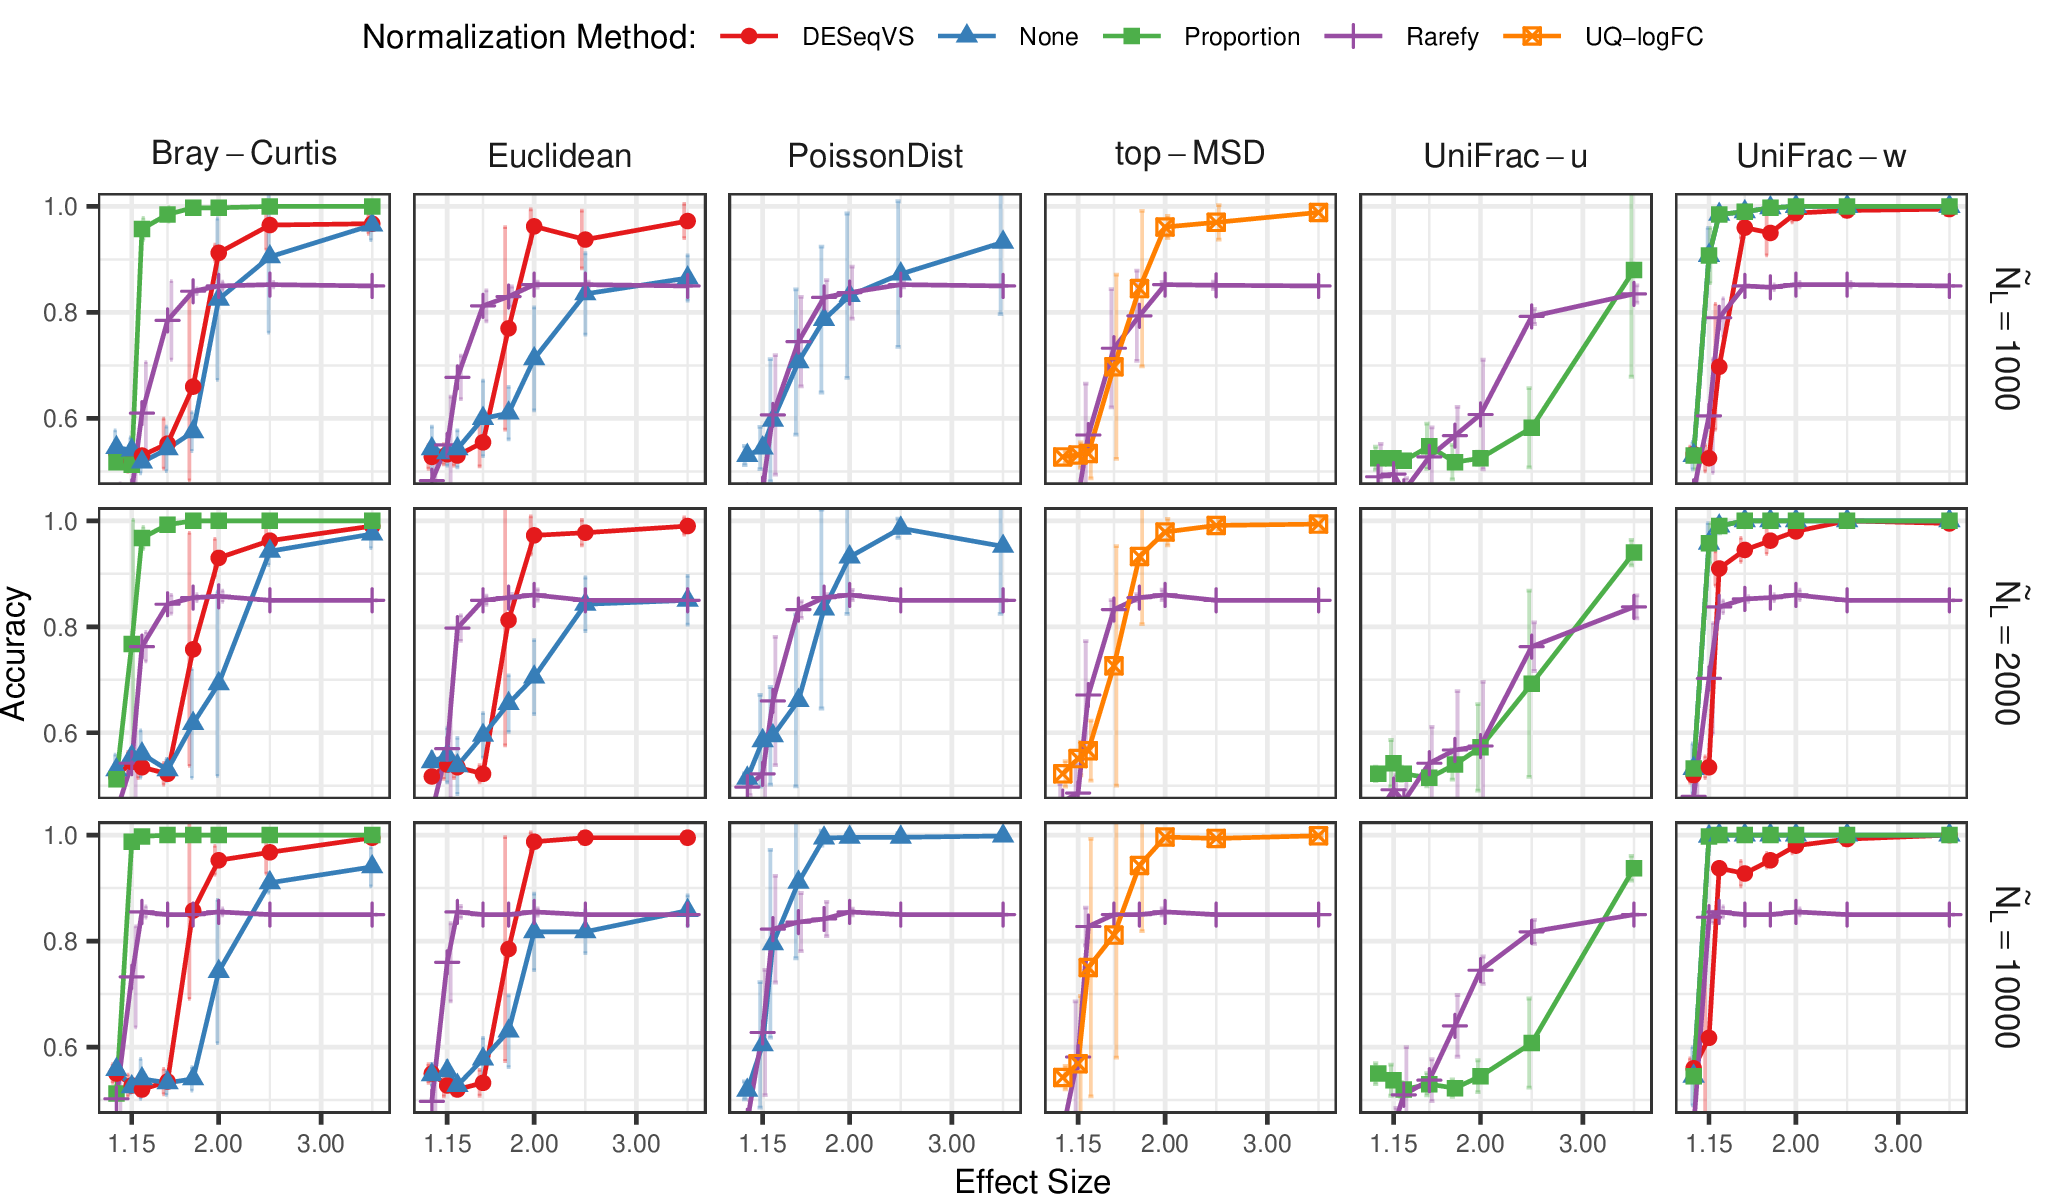
\includegraphics{figure_01.png}

\textbf{Figure 1. Re-running the R-flavored markdown provided in
Protocol S1 of WNWN qualitatively regenerated Figure 3 from the original
study.}

\newpage

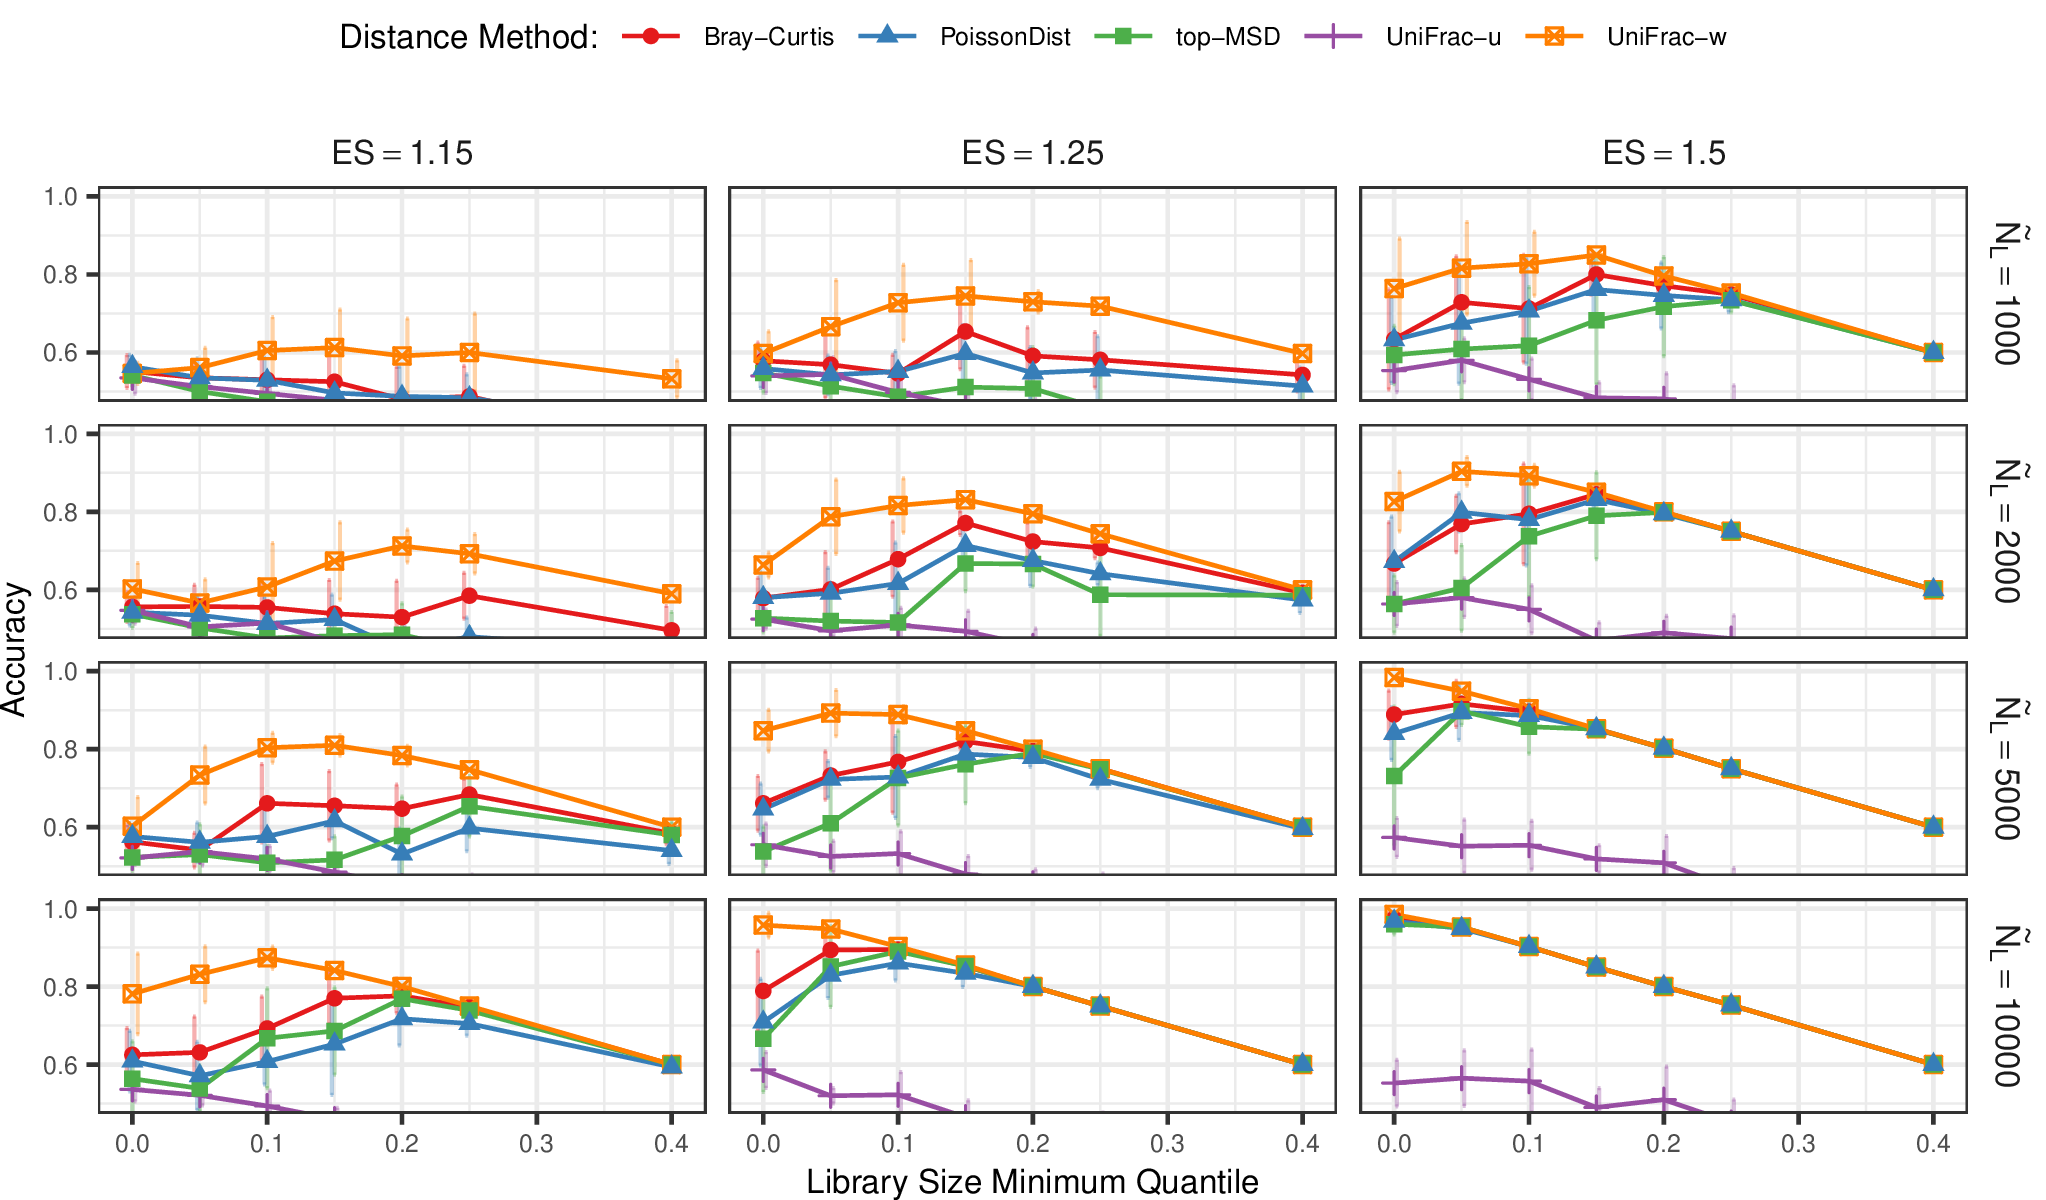
\includegraphics{figure_02.png}

\textbf{Figure 2. Re-running the R-flavored markdown provided in
Protocol S1 of WNWN qualitatively regenerated Figure 4 from the original
study.}

\newpage

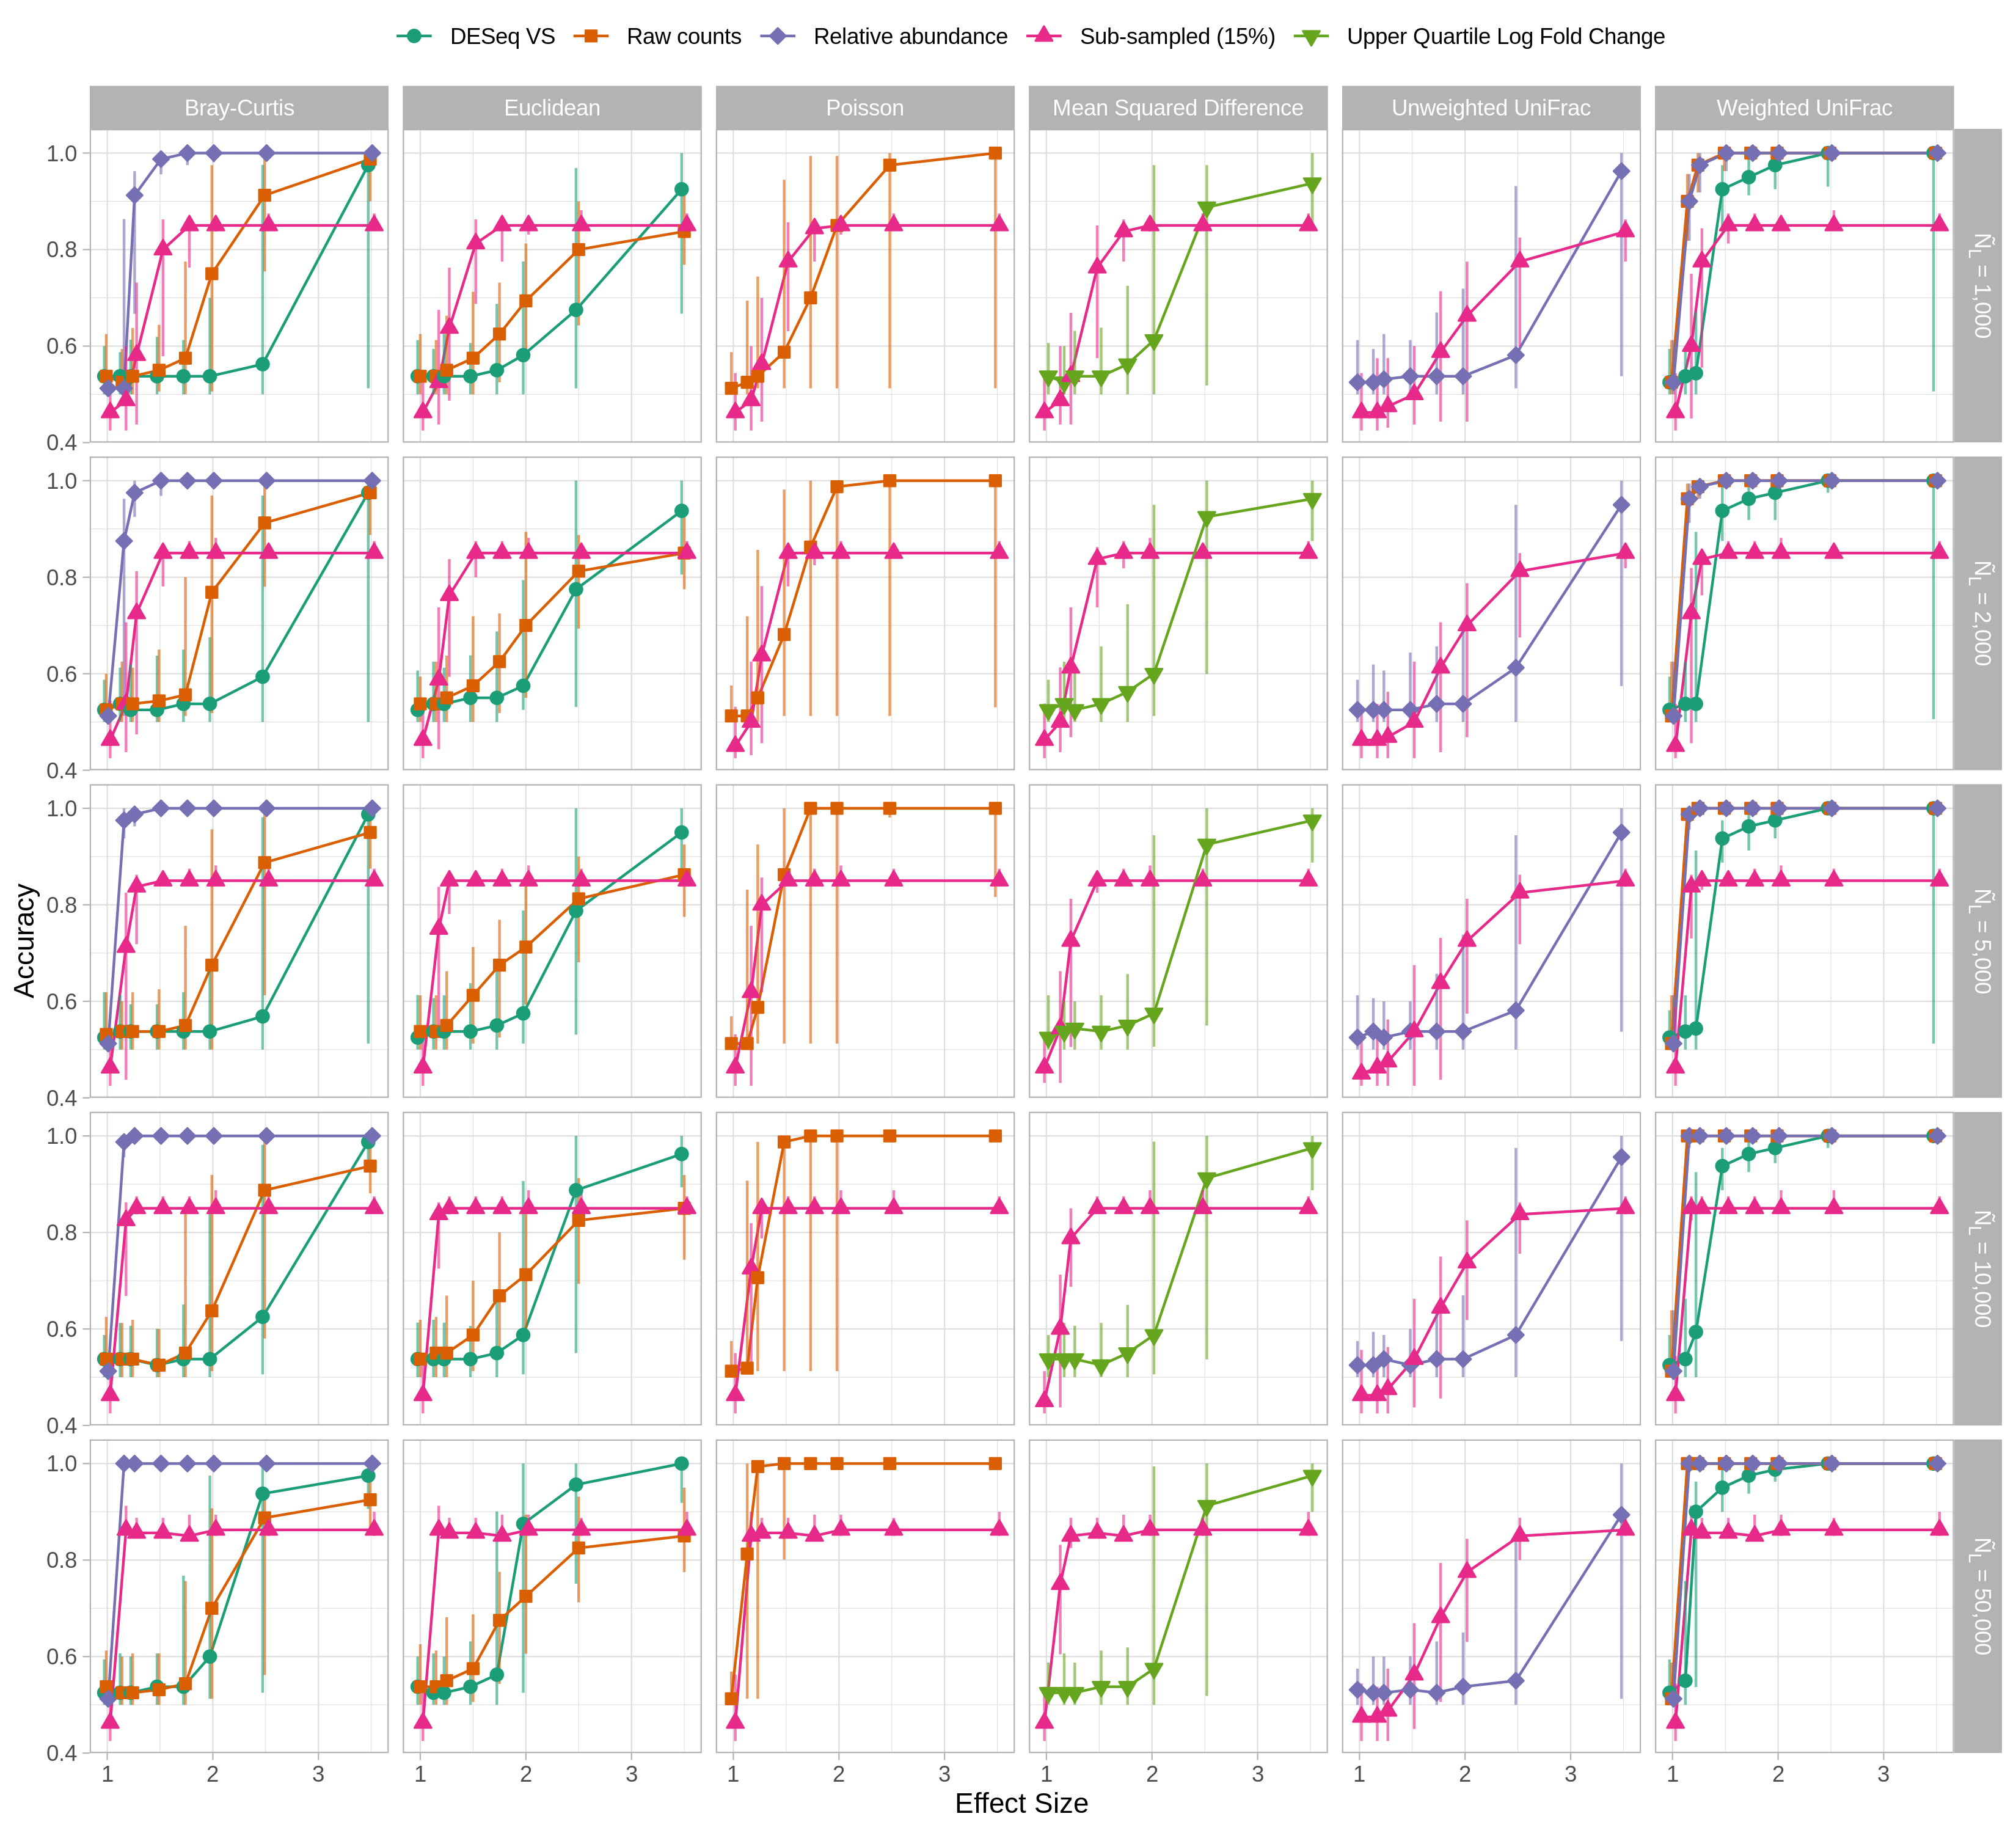
\includegraphics{figure_03.png}

\textbf{Figure 3. Successful reimplementation and expansion of analysis
presented in Figure 3 from WNWN in a Snakemake pipeline.} The
reimplemented workflow largely borrowed from the original
\texttt{simulation-cluster-accuracy-server.Rmd} R flavored markdown file
provided in WNWN's Protocol S1. The most notable differences include the
use of 100 rather than 5 randomizations and the addition of the median
sequencing depth (Ñ\textsubscript{L}) of 50,000. The plotting symbols
indicate the median of 100 randomizations and the error bars represent
the observed 95\% confidence interval. Simulations run at the same
effect size are dodged to better reveal overlapping data. The sequencing
depths were drawn from the GlobalPatterns dataset and sequences were
clusterd using PAM.

\newpage

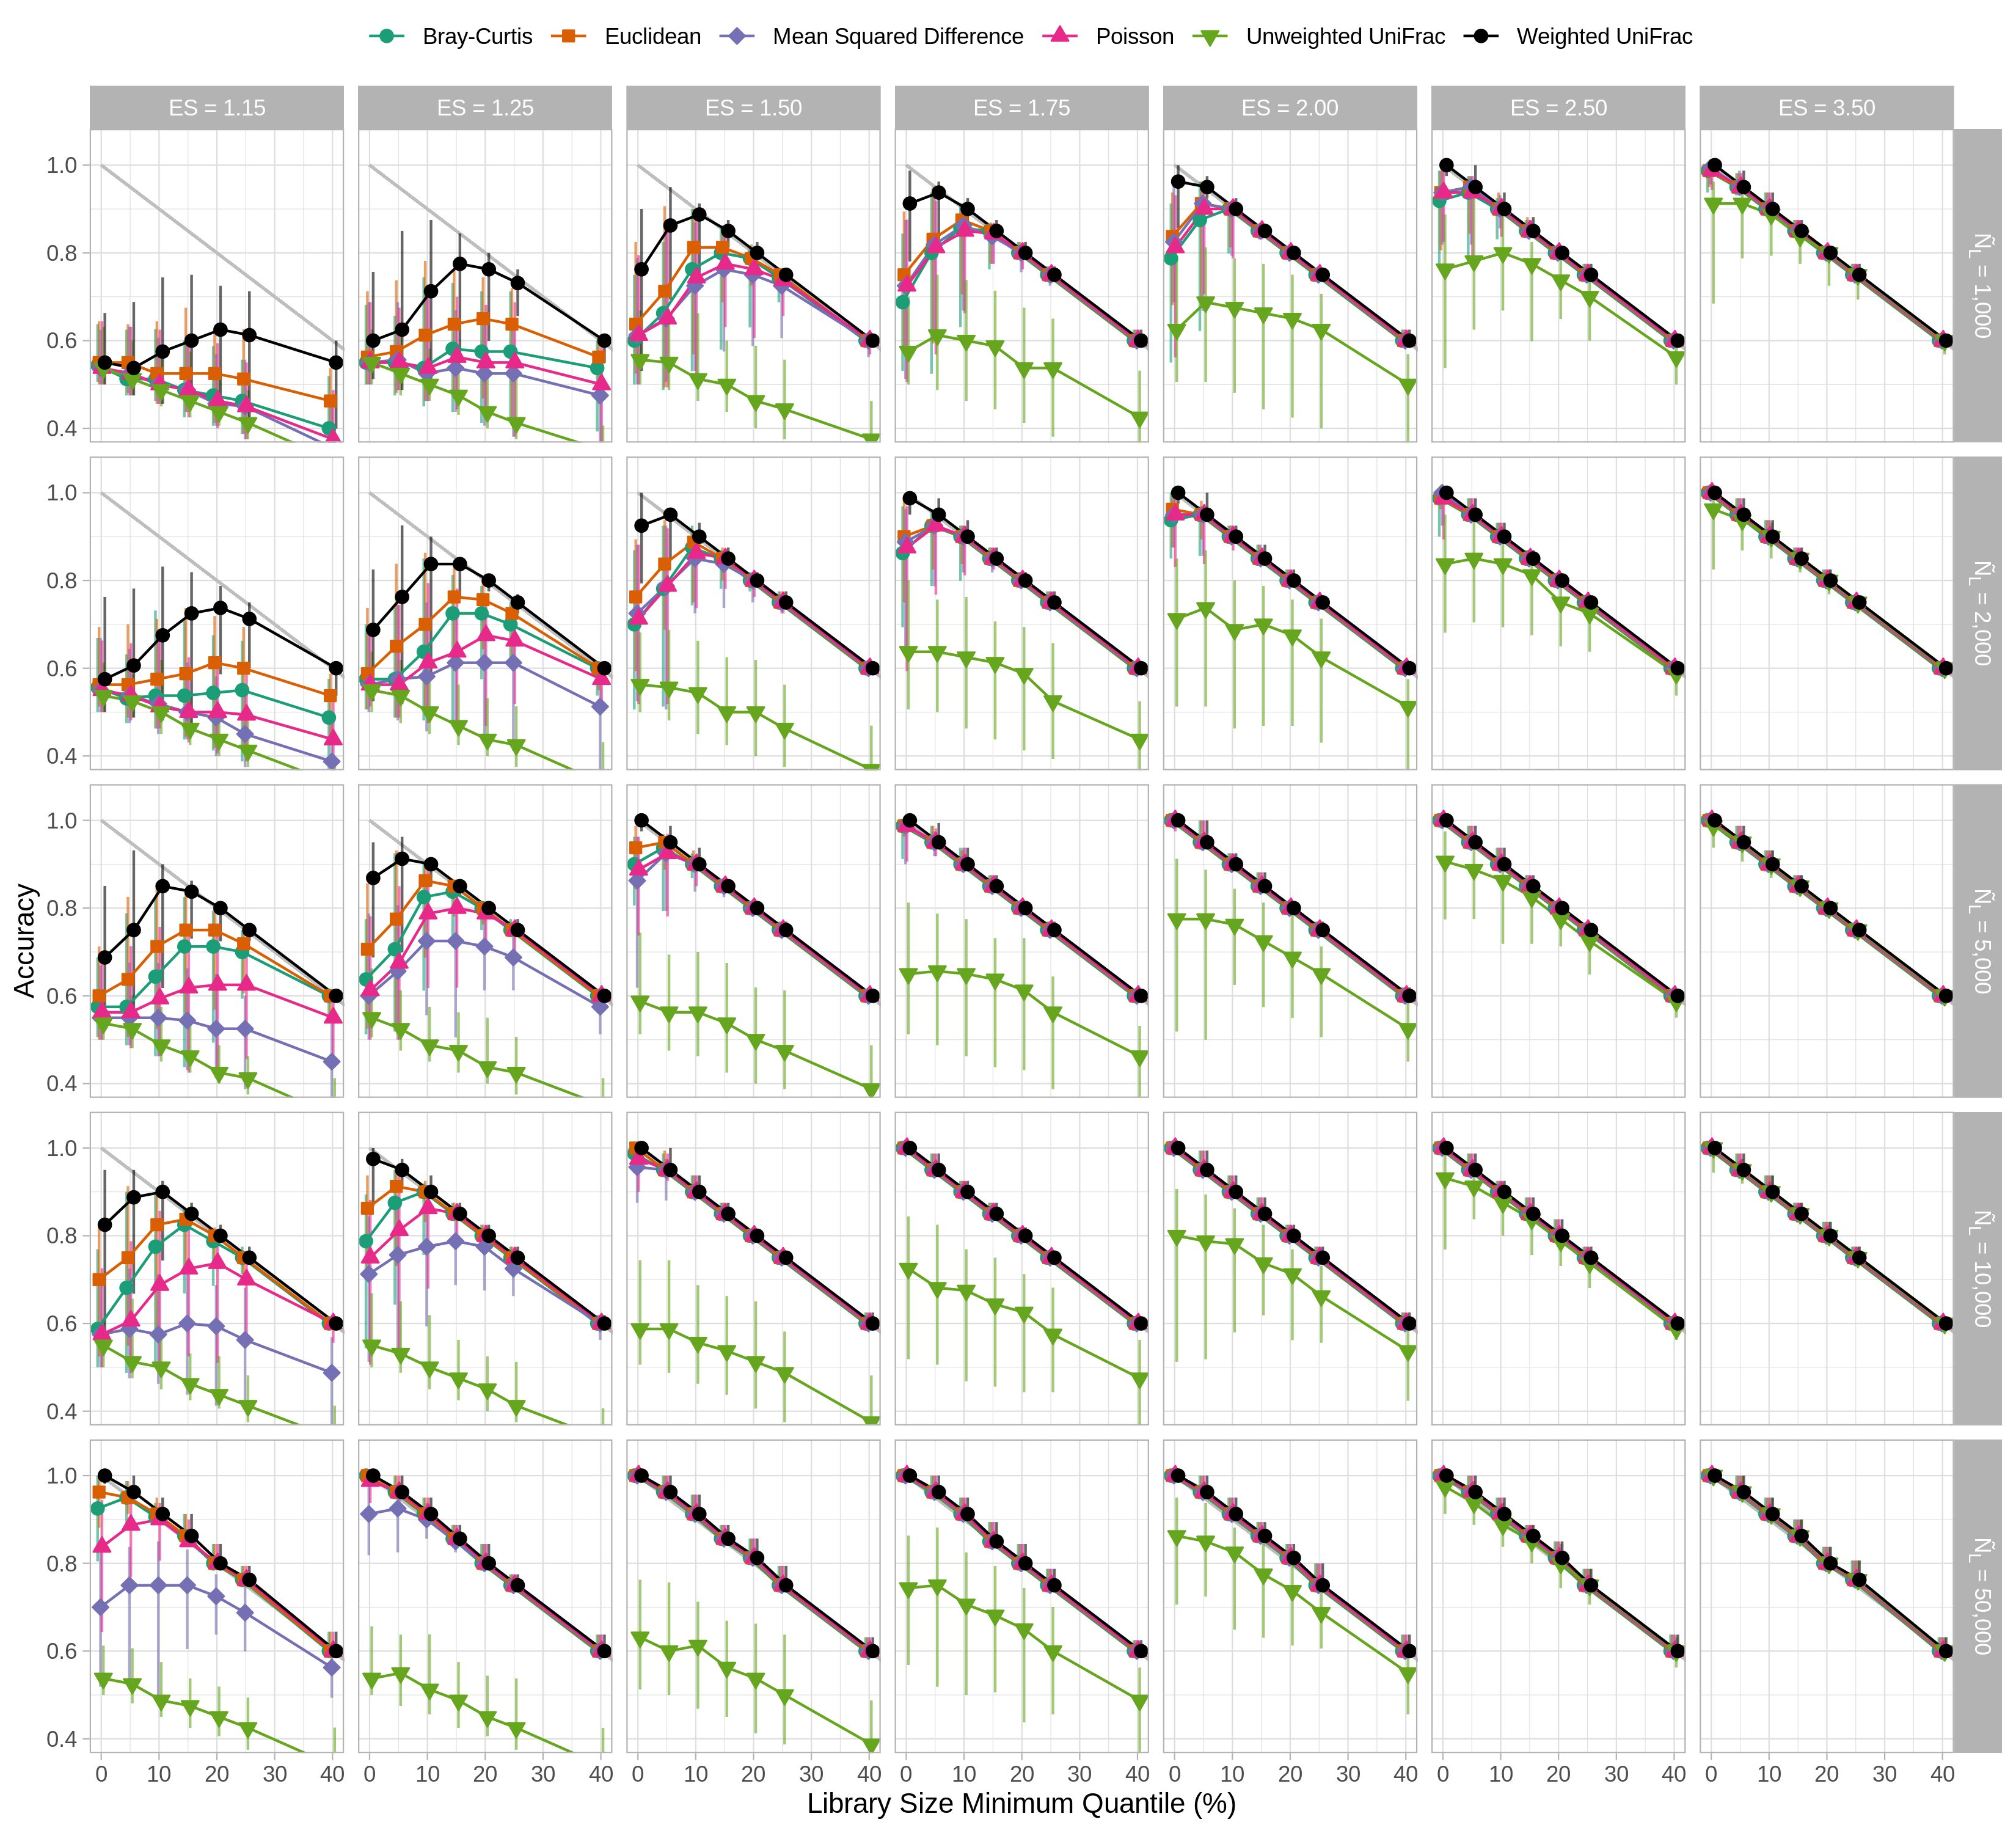
\includegraphics{figure_04.png}

\textbf{Figure 4. Successful reimplementation and expansion of analysis
presented in Figure 4 from WNWN in a Snakemake pipeline.} The
reimplemented workflow largely borrowed from the original
\texttt{simulation-cluster-accuracy-server.Rmd} R flavored markdown file
provided in WNWN's Protocol S1. The most notable differences include the
use of 100 rather than 5 randomizations and the addition of the median
sequencing depth (Ñ\textsubscript{L}) of 50,000. The plotting symbols
indicate the median of 100 randomizations and the error bars represent
the observed 95\% confidence interval. Simulations run at the same
effect size are dodged to better reveal overlapping data. The sequencing
depths were drawn from the GlobalPatterns dataset and sequences were
clusterd using PAM.

\newpage

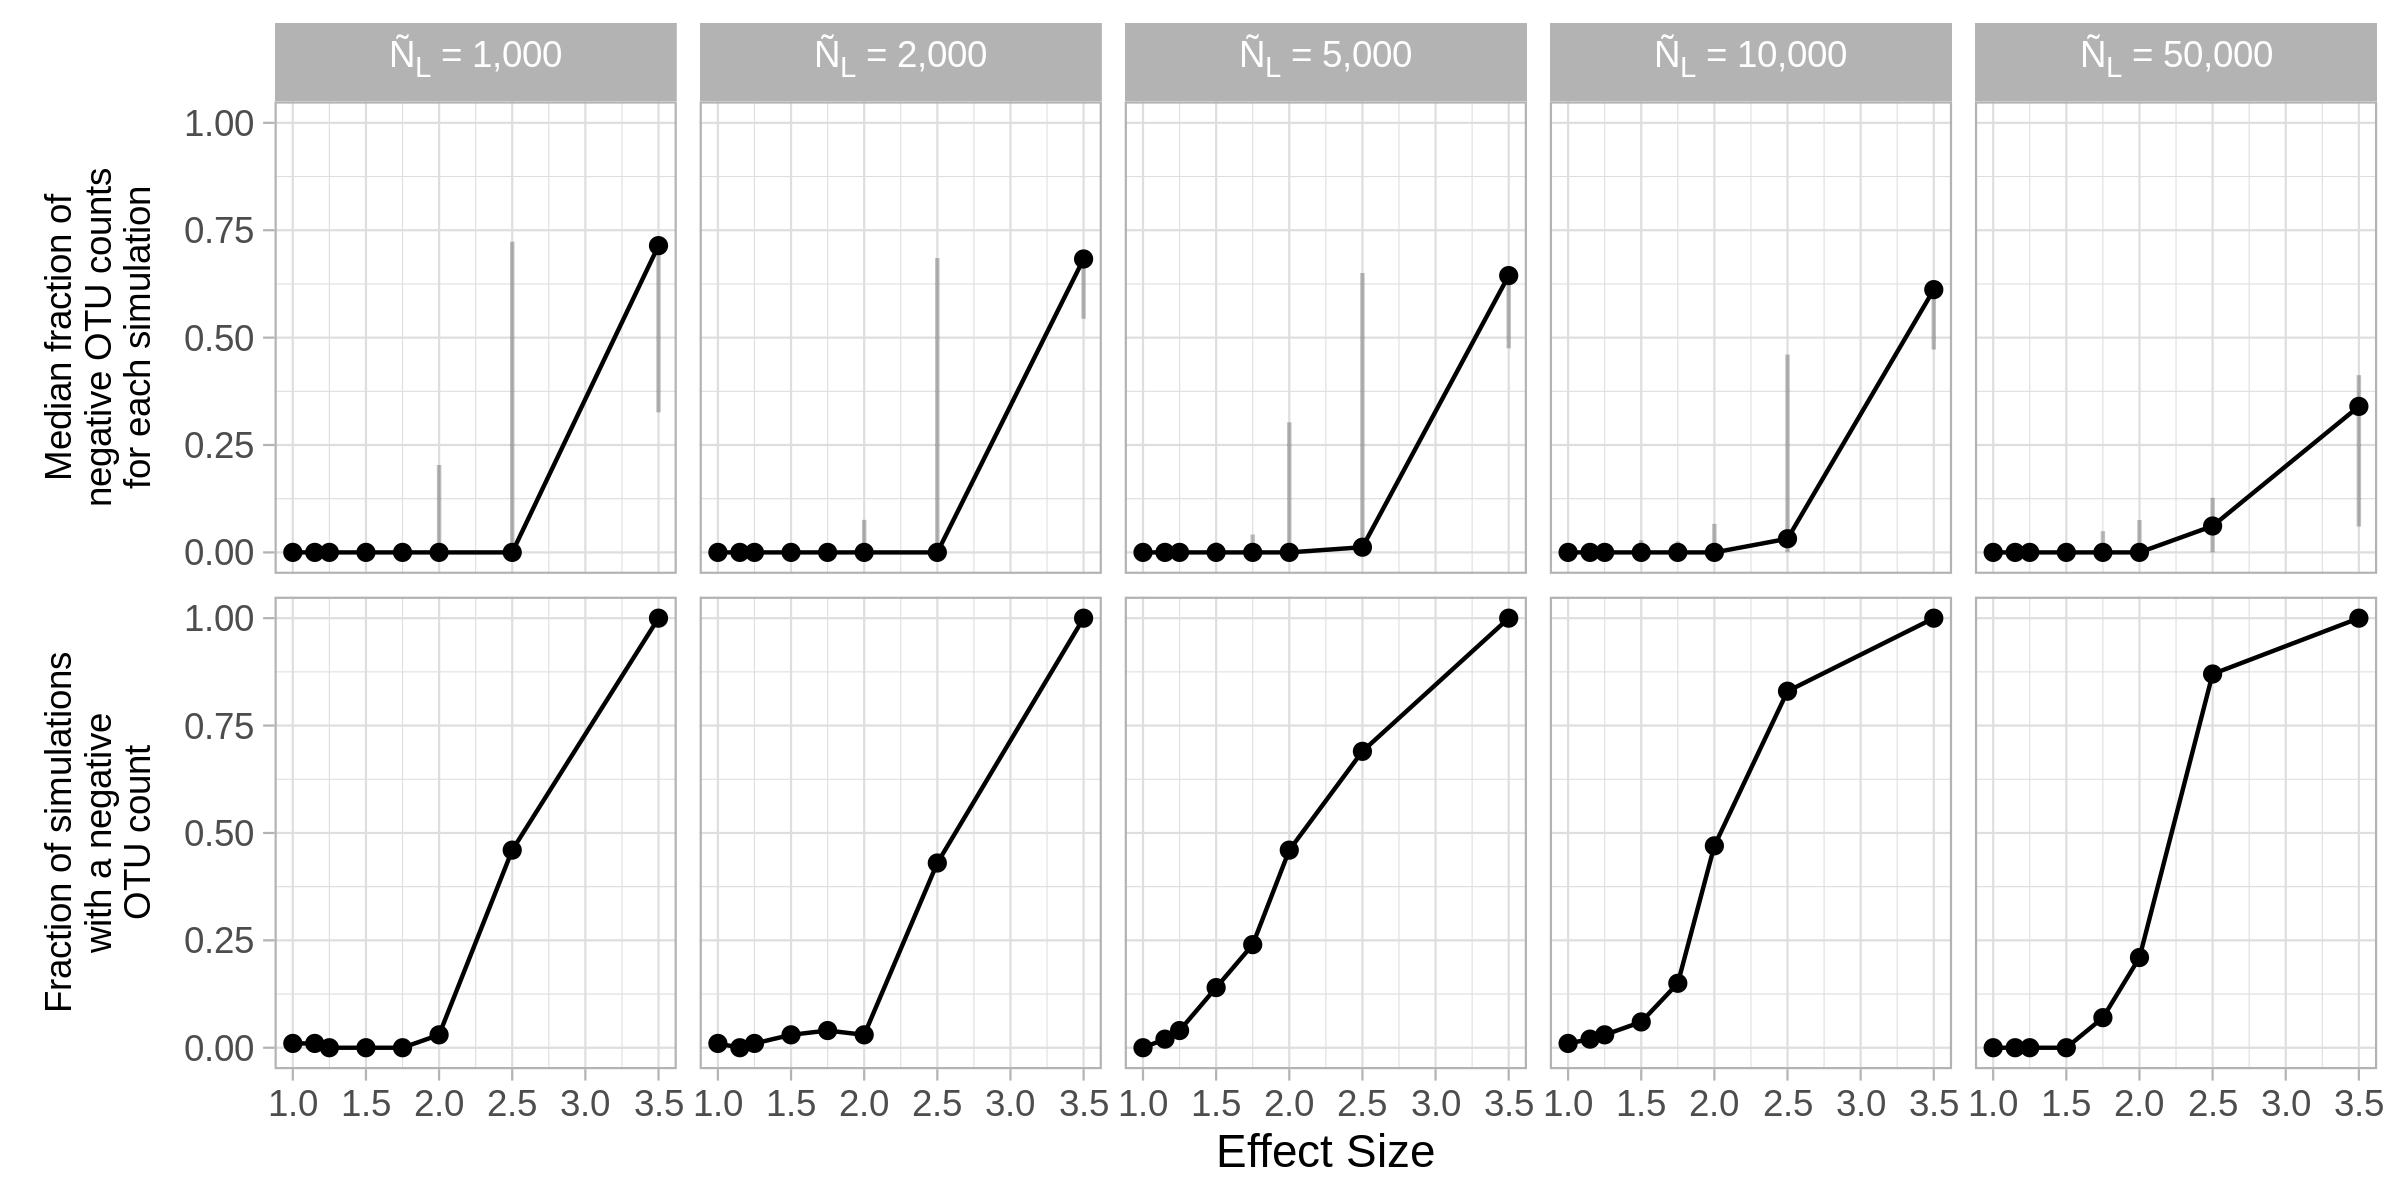
\includegraphics{figure_05.png}

\textbf{Figure 5. DESeq Variance Stabilization of OTU counts resulted in
negative values that were used to calculate Bray-Curtis and Weighted
UniFrac distances.} The median number of negative OTU counts that had a
negative OTU count following normalization increased with the effect
size and decreased as Ñ\textsubscript{L} increased. The fraction
simulated datasets that had a negative OTU count following normalization
also increased with effect size, but increased as Ñ\textsubscript{L}
increased. For each effect size there were 100 replicate datasets. The
error bars indicate the observe 95\% confidence interval.

\newpage

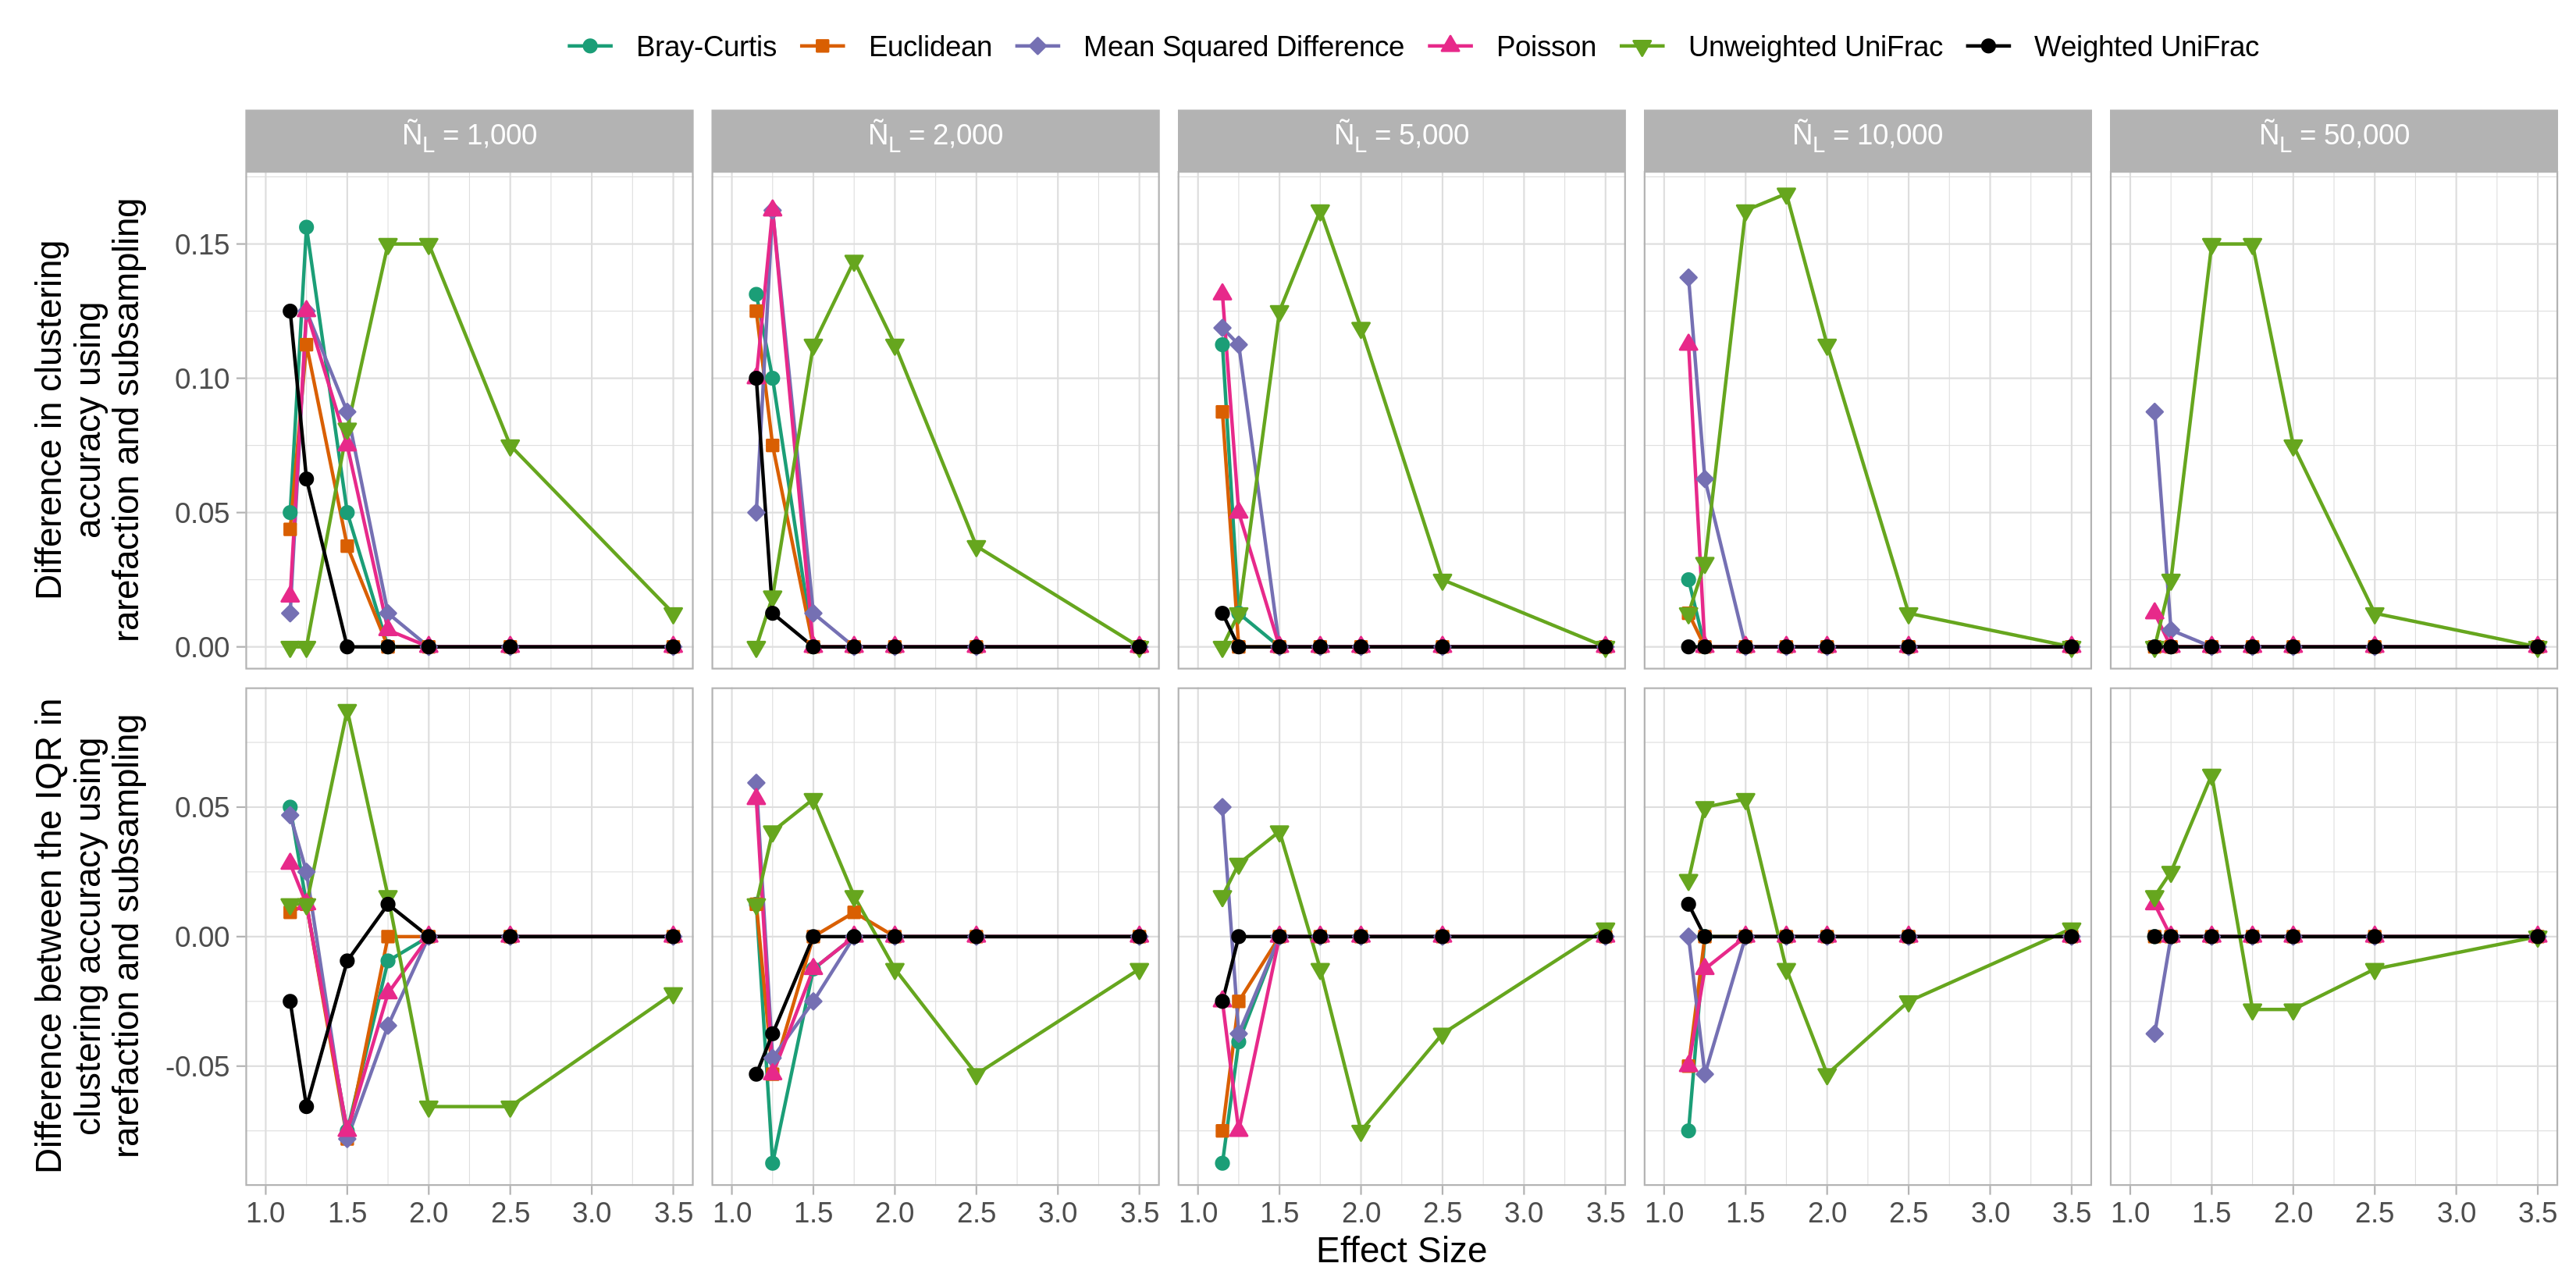
\includegraphics{figure_06.png}

\textbf{Figure 6. Rarefaction resulted in larger and less variable
clustering accuracies.} With the exception of Unweighted UniFrac
distances, the improved performance by rarefaction was observed at
smaller effect sizes. In the first row of panels larger values mean that
the accuracies by rarefaction were better than those of subsampling. In
the second row of samples, larger values mean that interquartile range
(IQR) for rarefaction was larger than that of subsampling.

\newpage

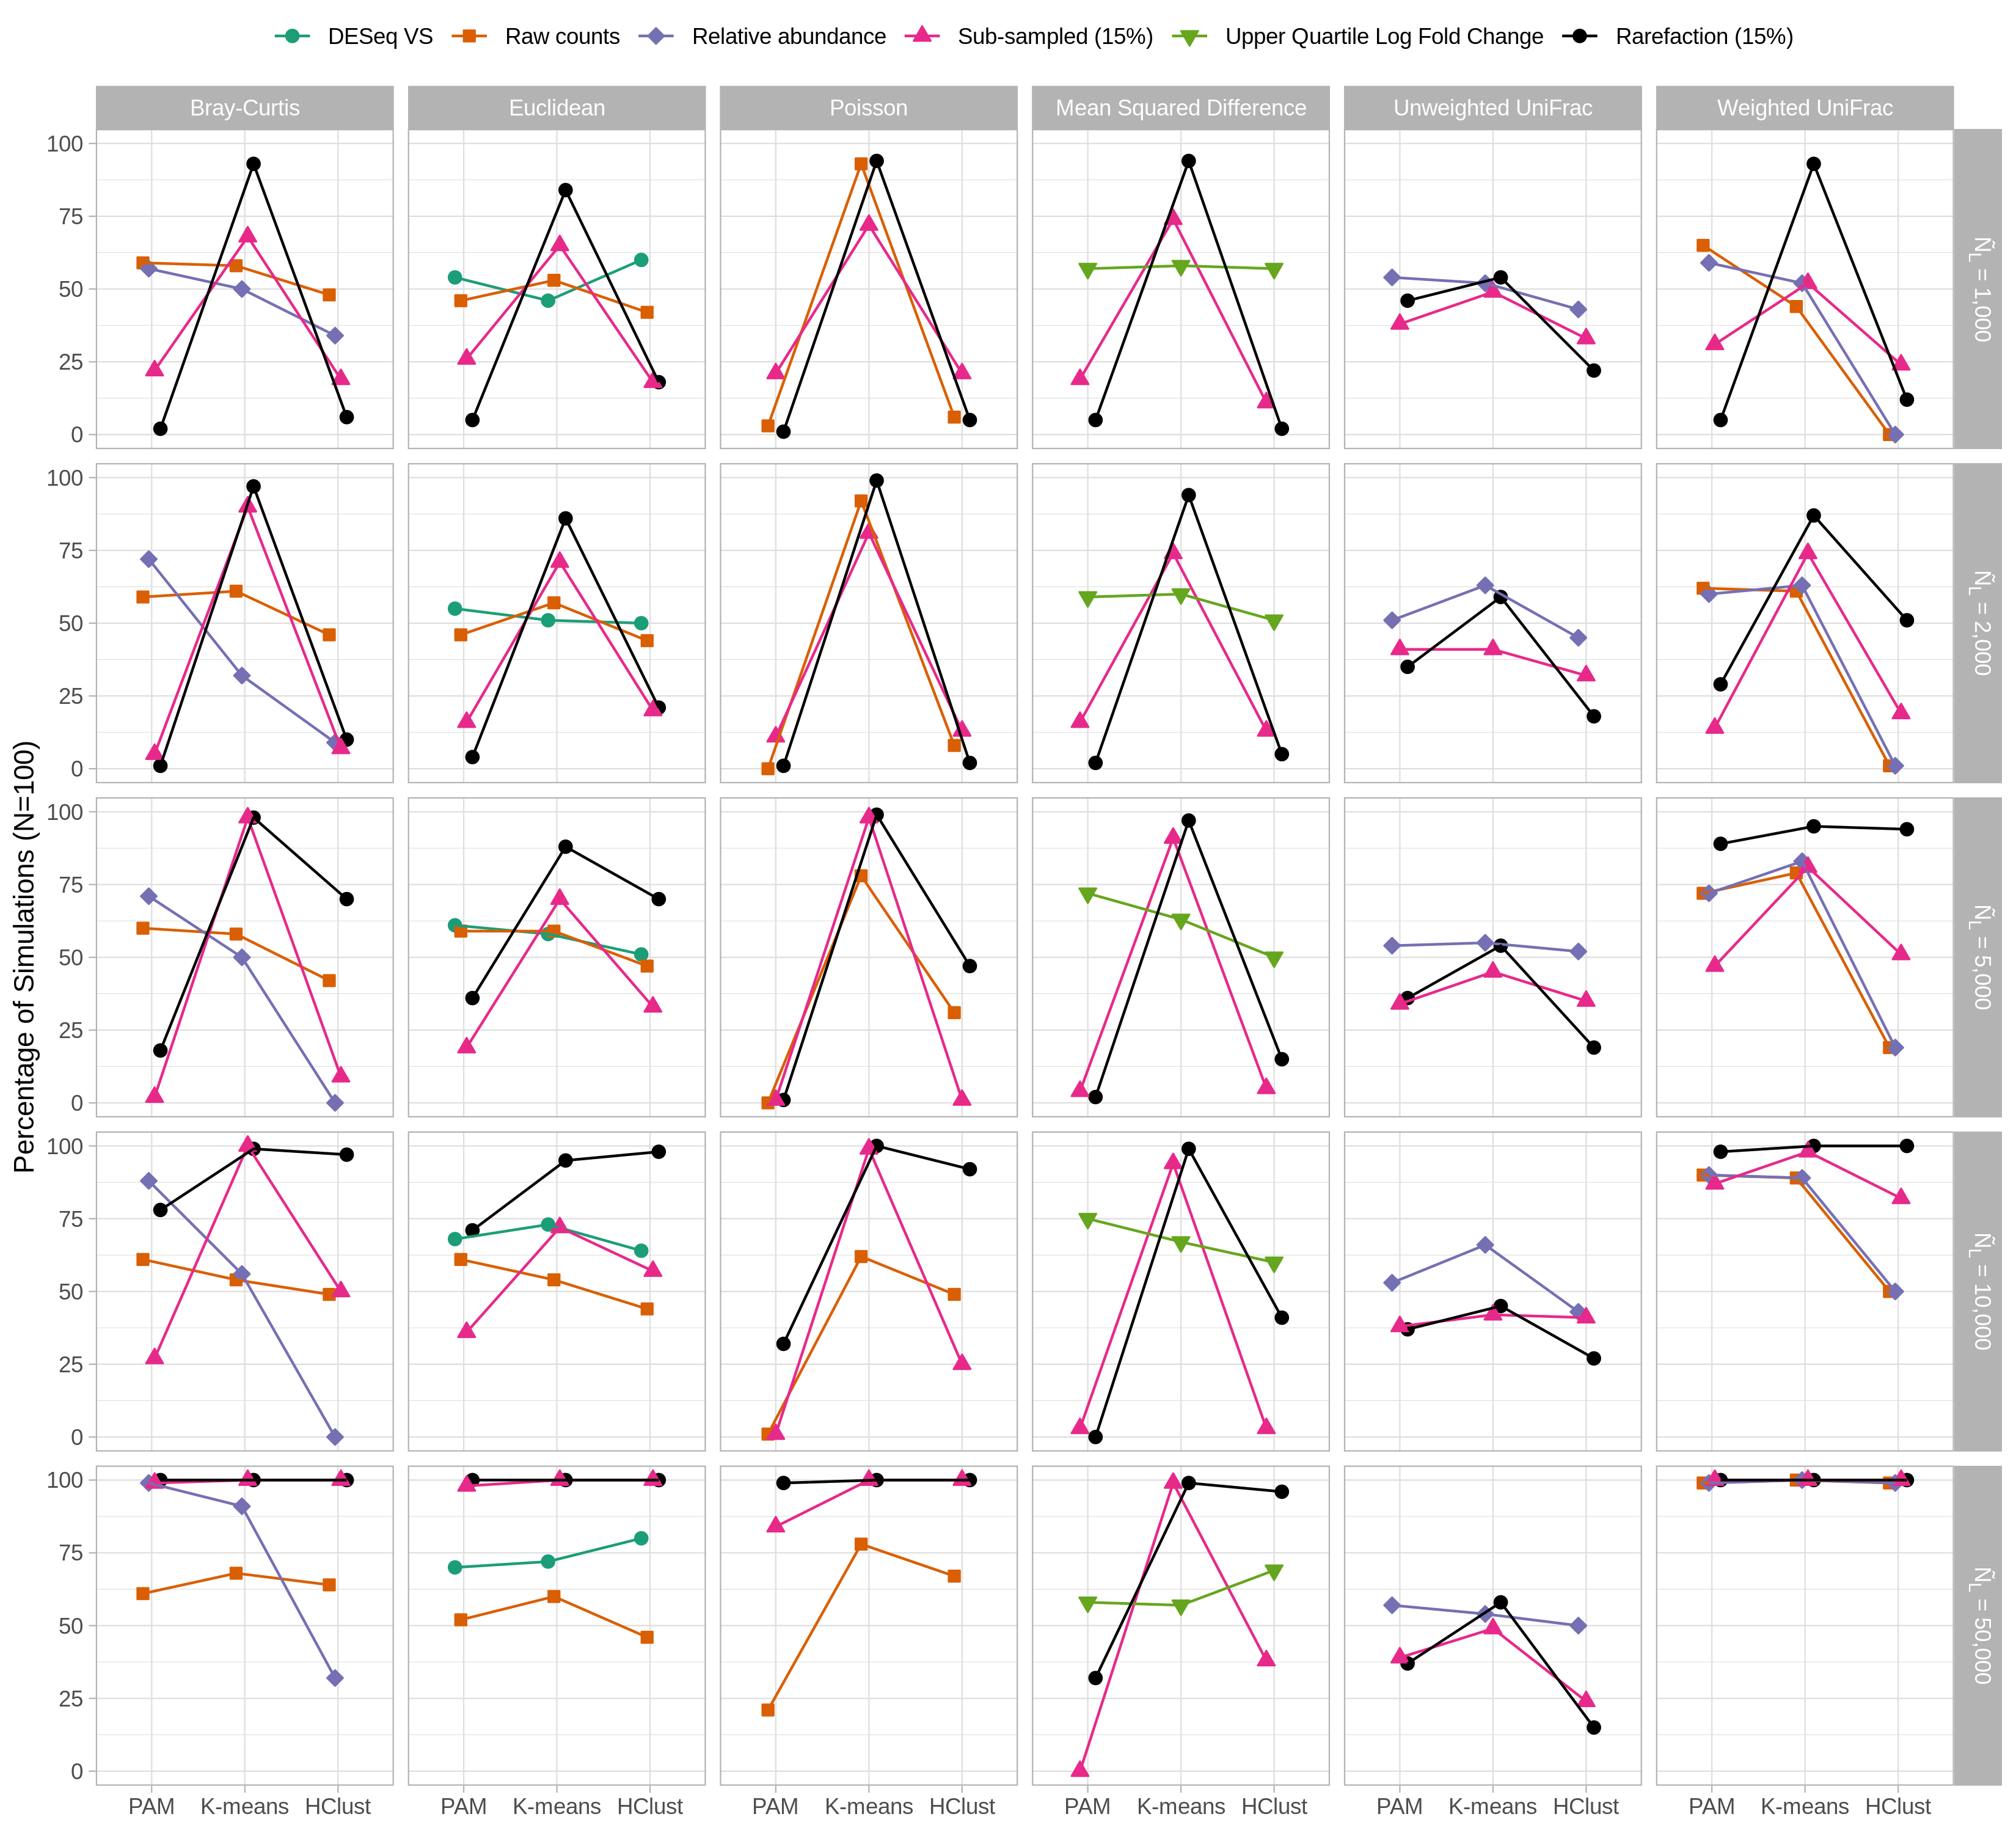
\includegraphics{figure_07.png}

\textbf{Figure 7. K-means clustering was consistently as good or better
than PAM or hierarchical clustering when comparing rarefaction to other
normalization methods.} Each point represents the percentage of 100
simulations where that clustering method performed as well or better
than the other methods for that normalization procedure.

\newpage

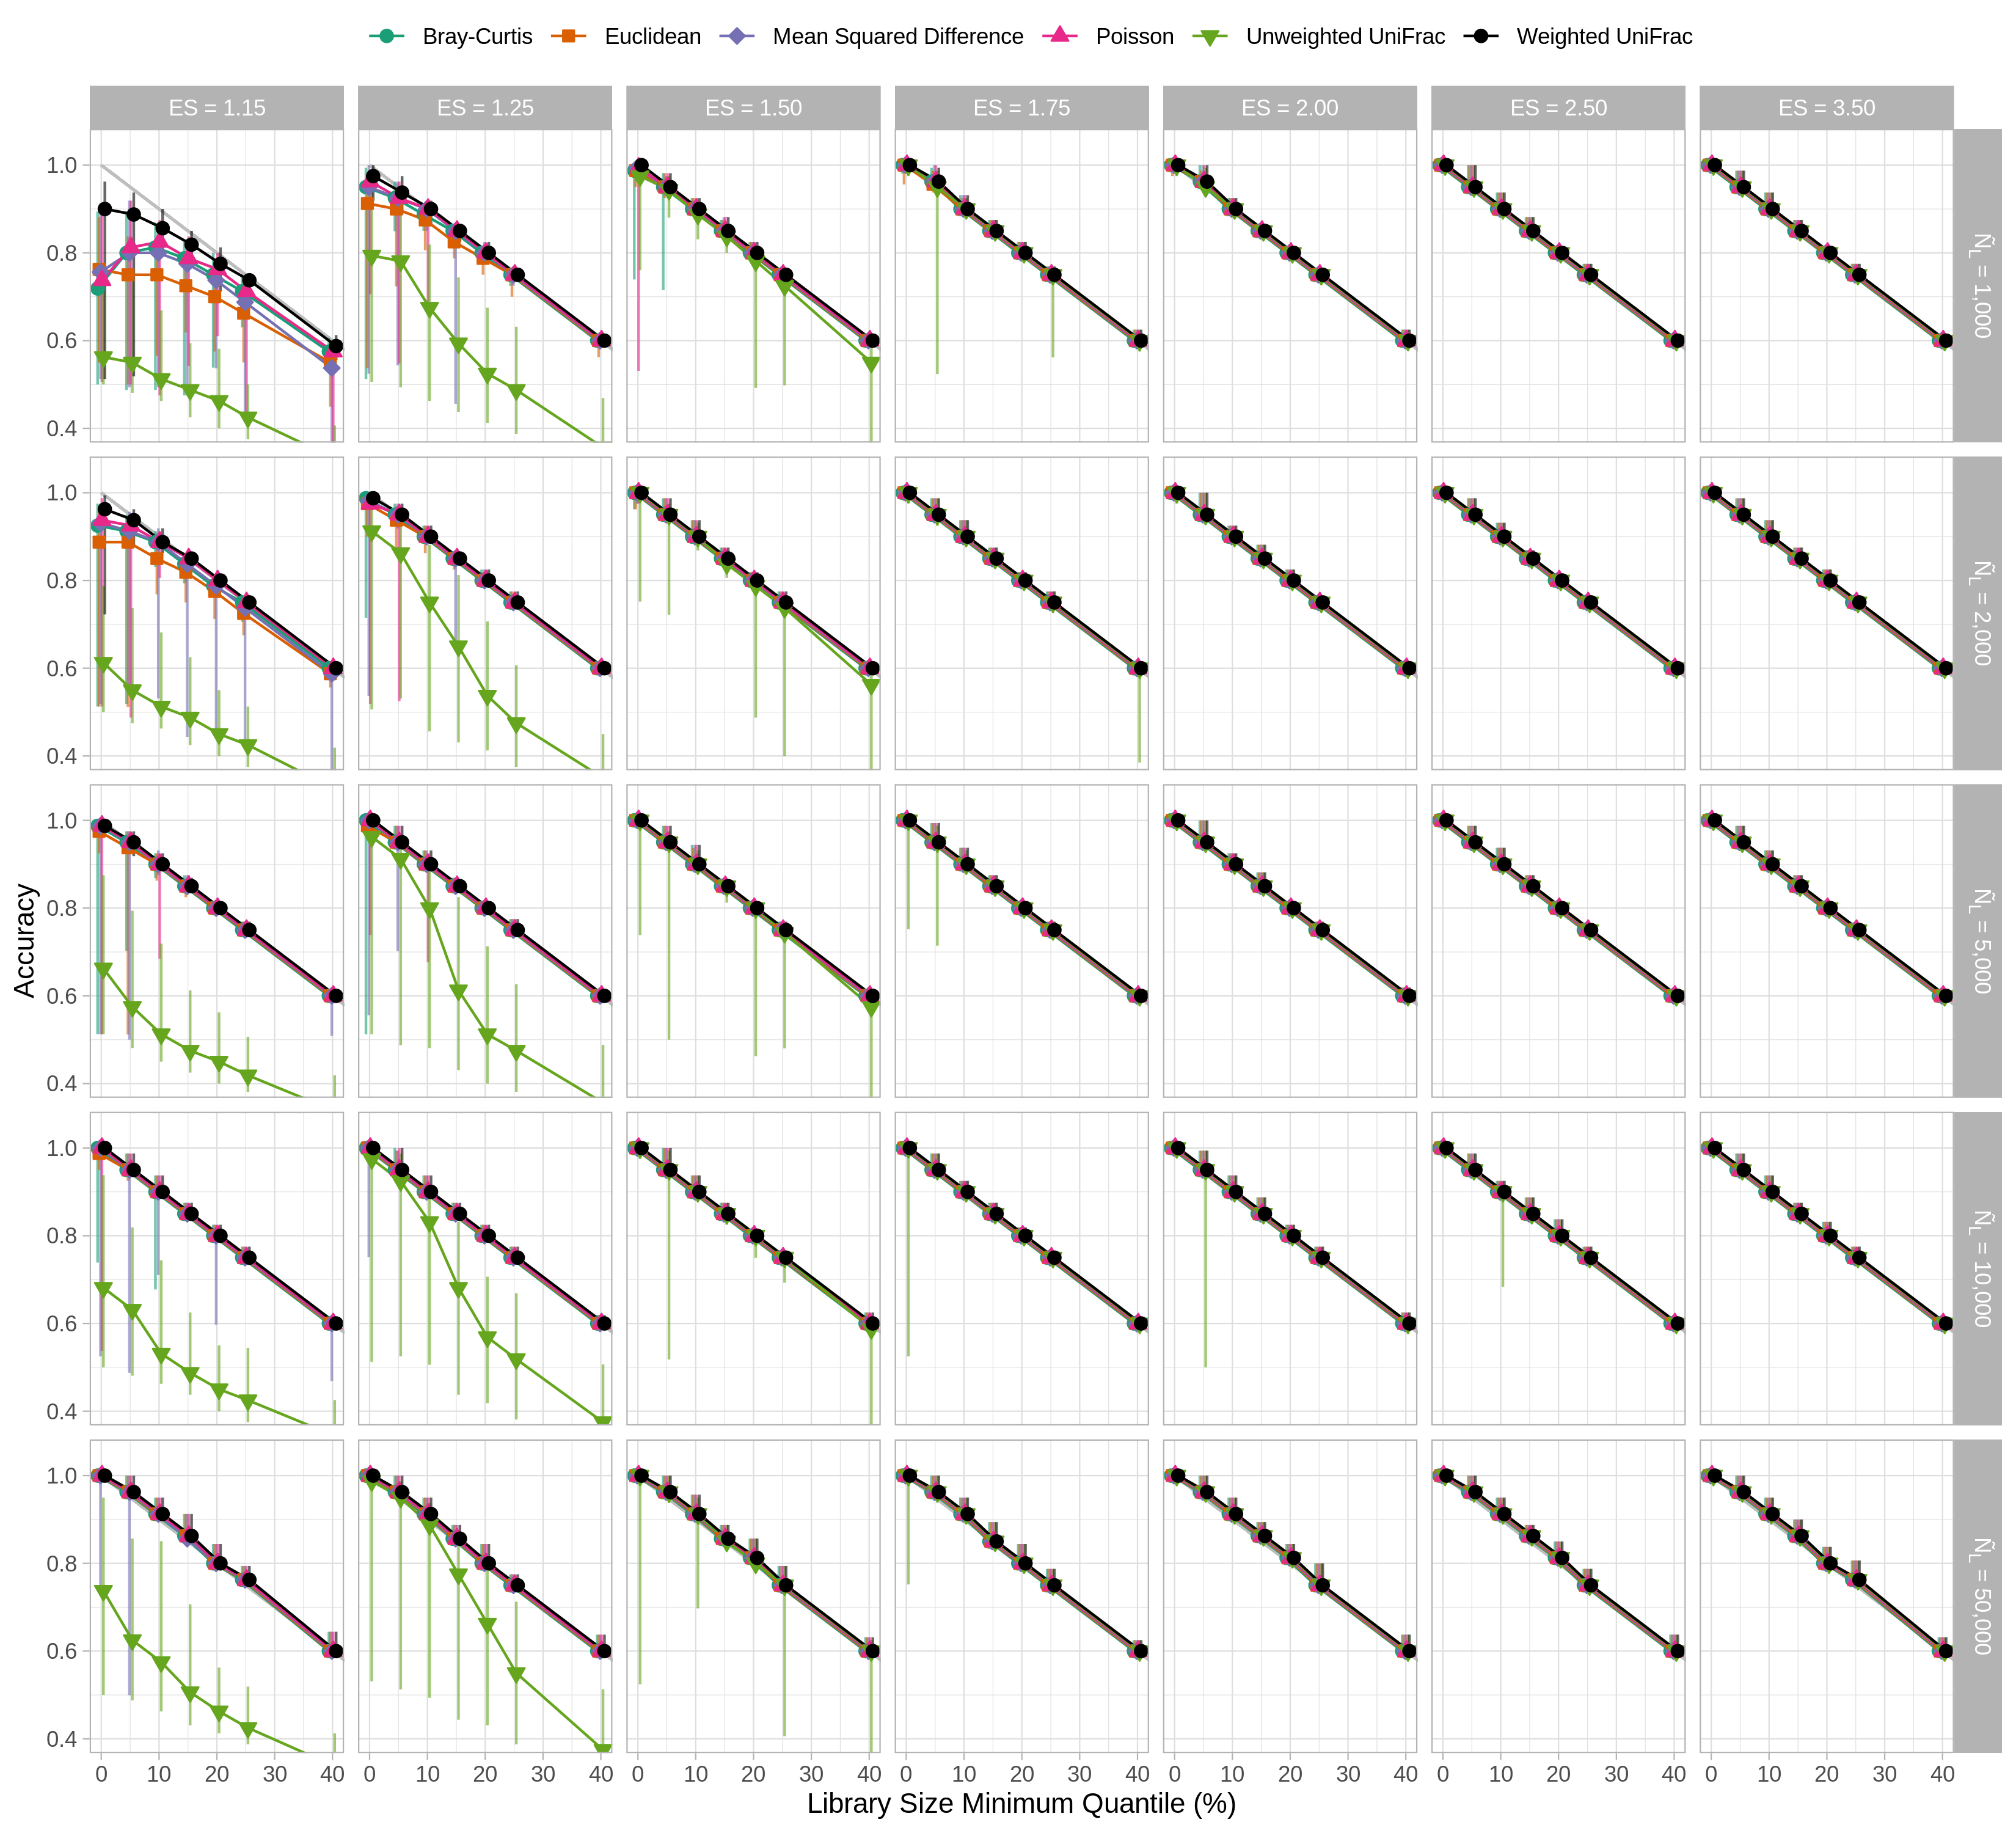
\includegraphics{figure_08.png}

\textbf{Figure 8. When the median sequencing depth was 2,000 sequences
or more, rarefaction of the entire dataset performed better than
removing the smallest 15\% of samples when using K-means clustering.}
This figure is analogous to Figure 4 except that K-means clustering was
used instead of PAM.

\newpage

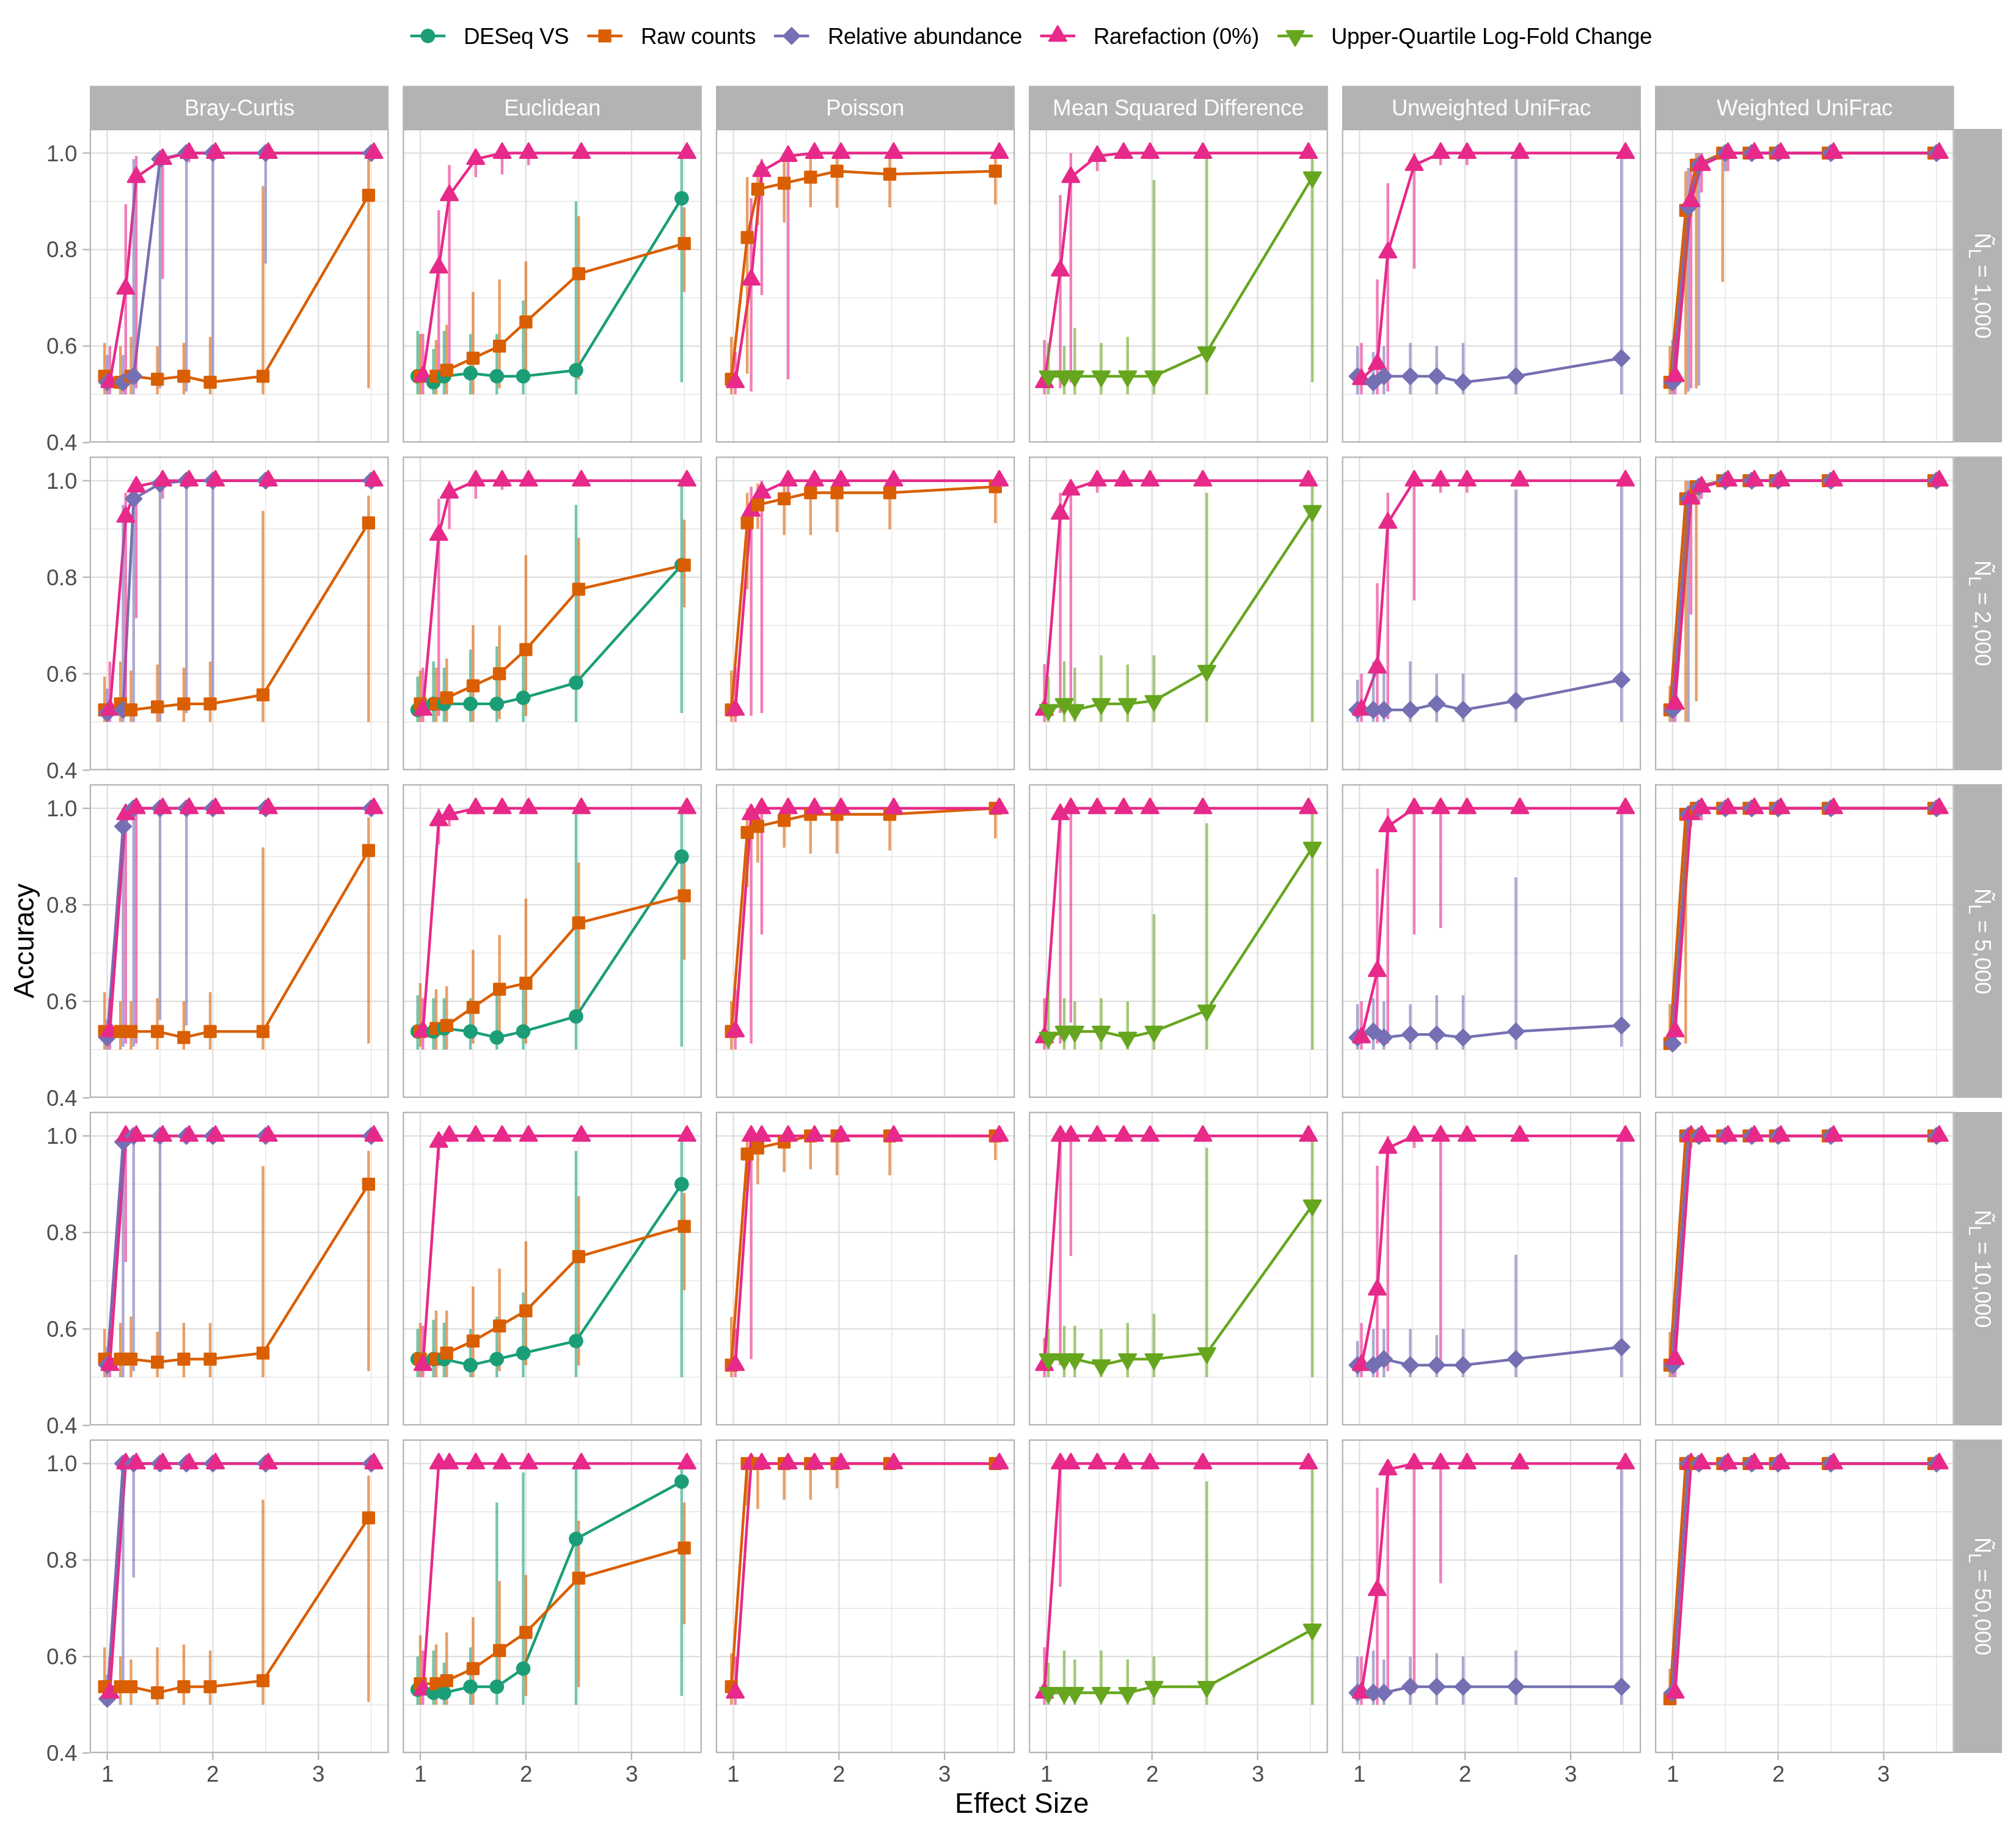
\includegraphics{figure_09.png}

\textbf{Figure 9. K-means clustering of distances calculated with
rarefaction were as good or better than any other normalization method.}
This figure is analogous to Figure 3 except that K-means clustering was
used instead of PAM, rarefaction on the full dataset was used instead of
subsampling to the size of the sample at the 15th percentile, and DESeq
variance stabilization normalized OTU counts were only used with
Euclidean distances.

\newpage

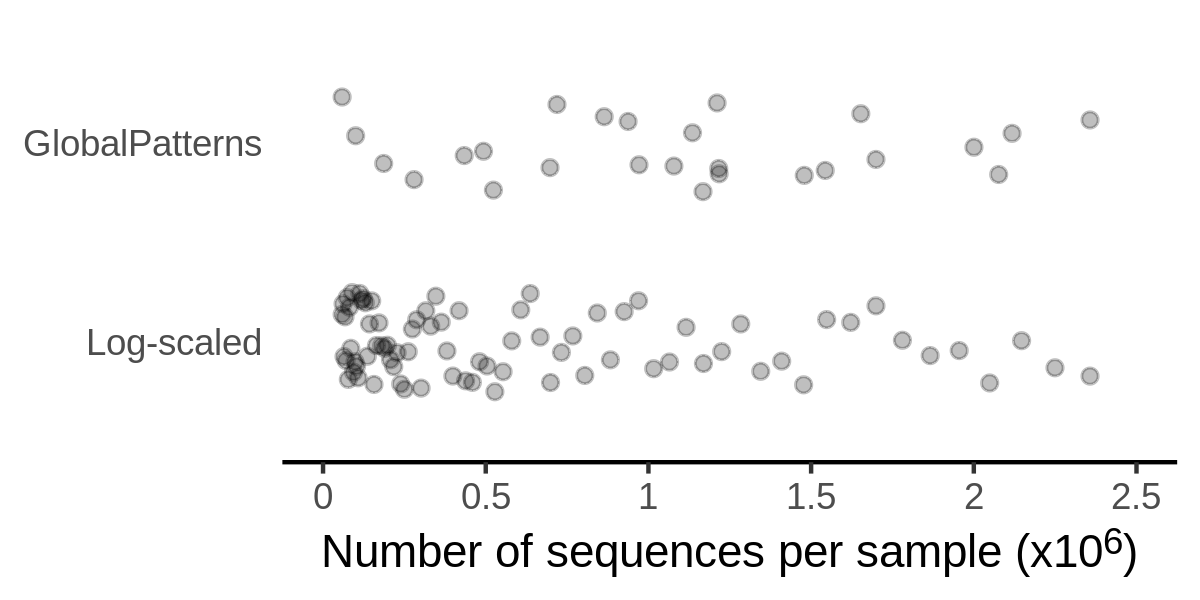
\includegraphics{figure_10.png}

\textbf{Figure 10. Comparison of the normally distributed sequencing
depths from the GlobalPatterns dataset and a log-scaled distribution of
sequencing depths.} The log-scaled distribution was generated so that
each sample in a simulation could have a unqiue number of sequences and
to simulate the skew right distribution commonly seen in microbiome
studies.

\newpage

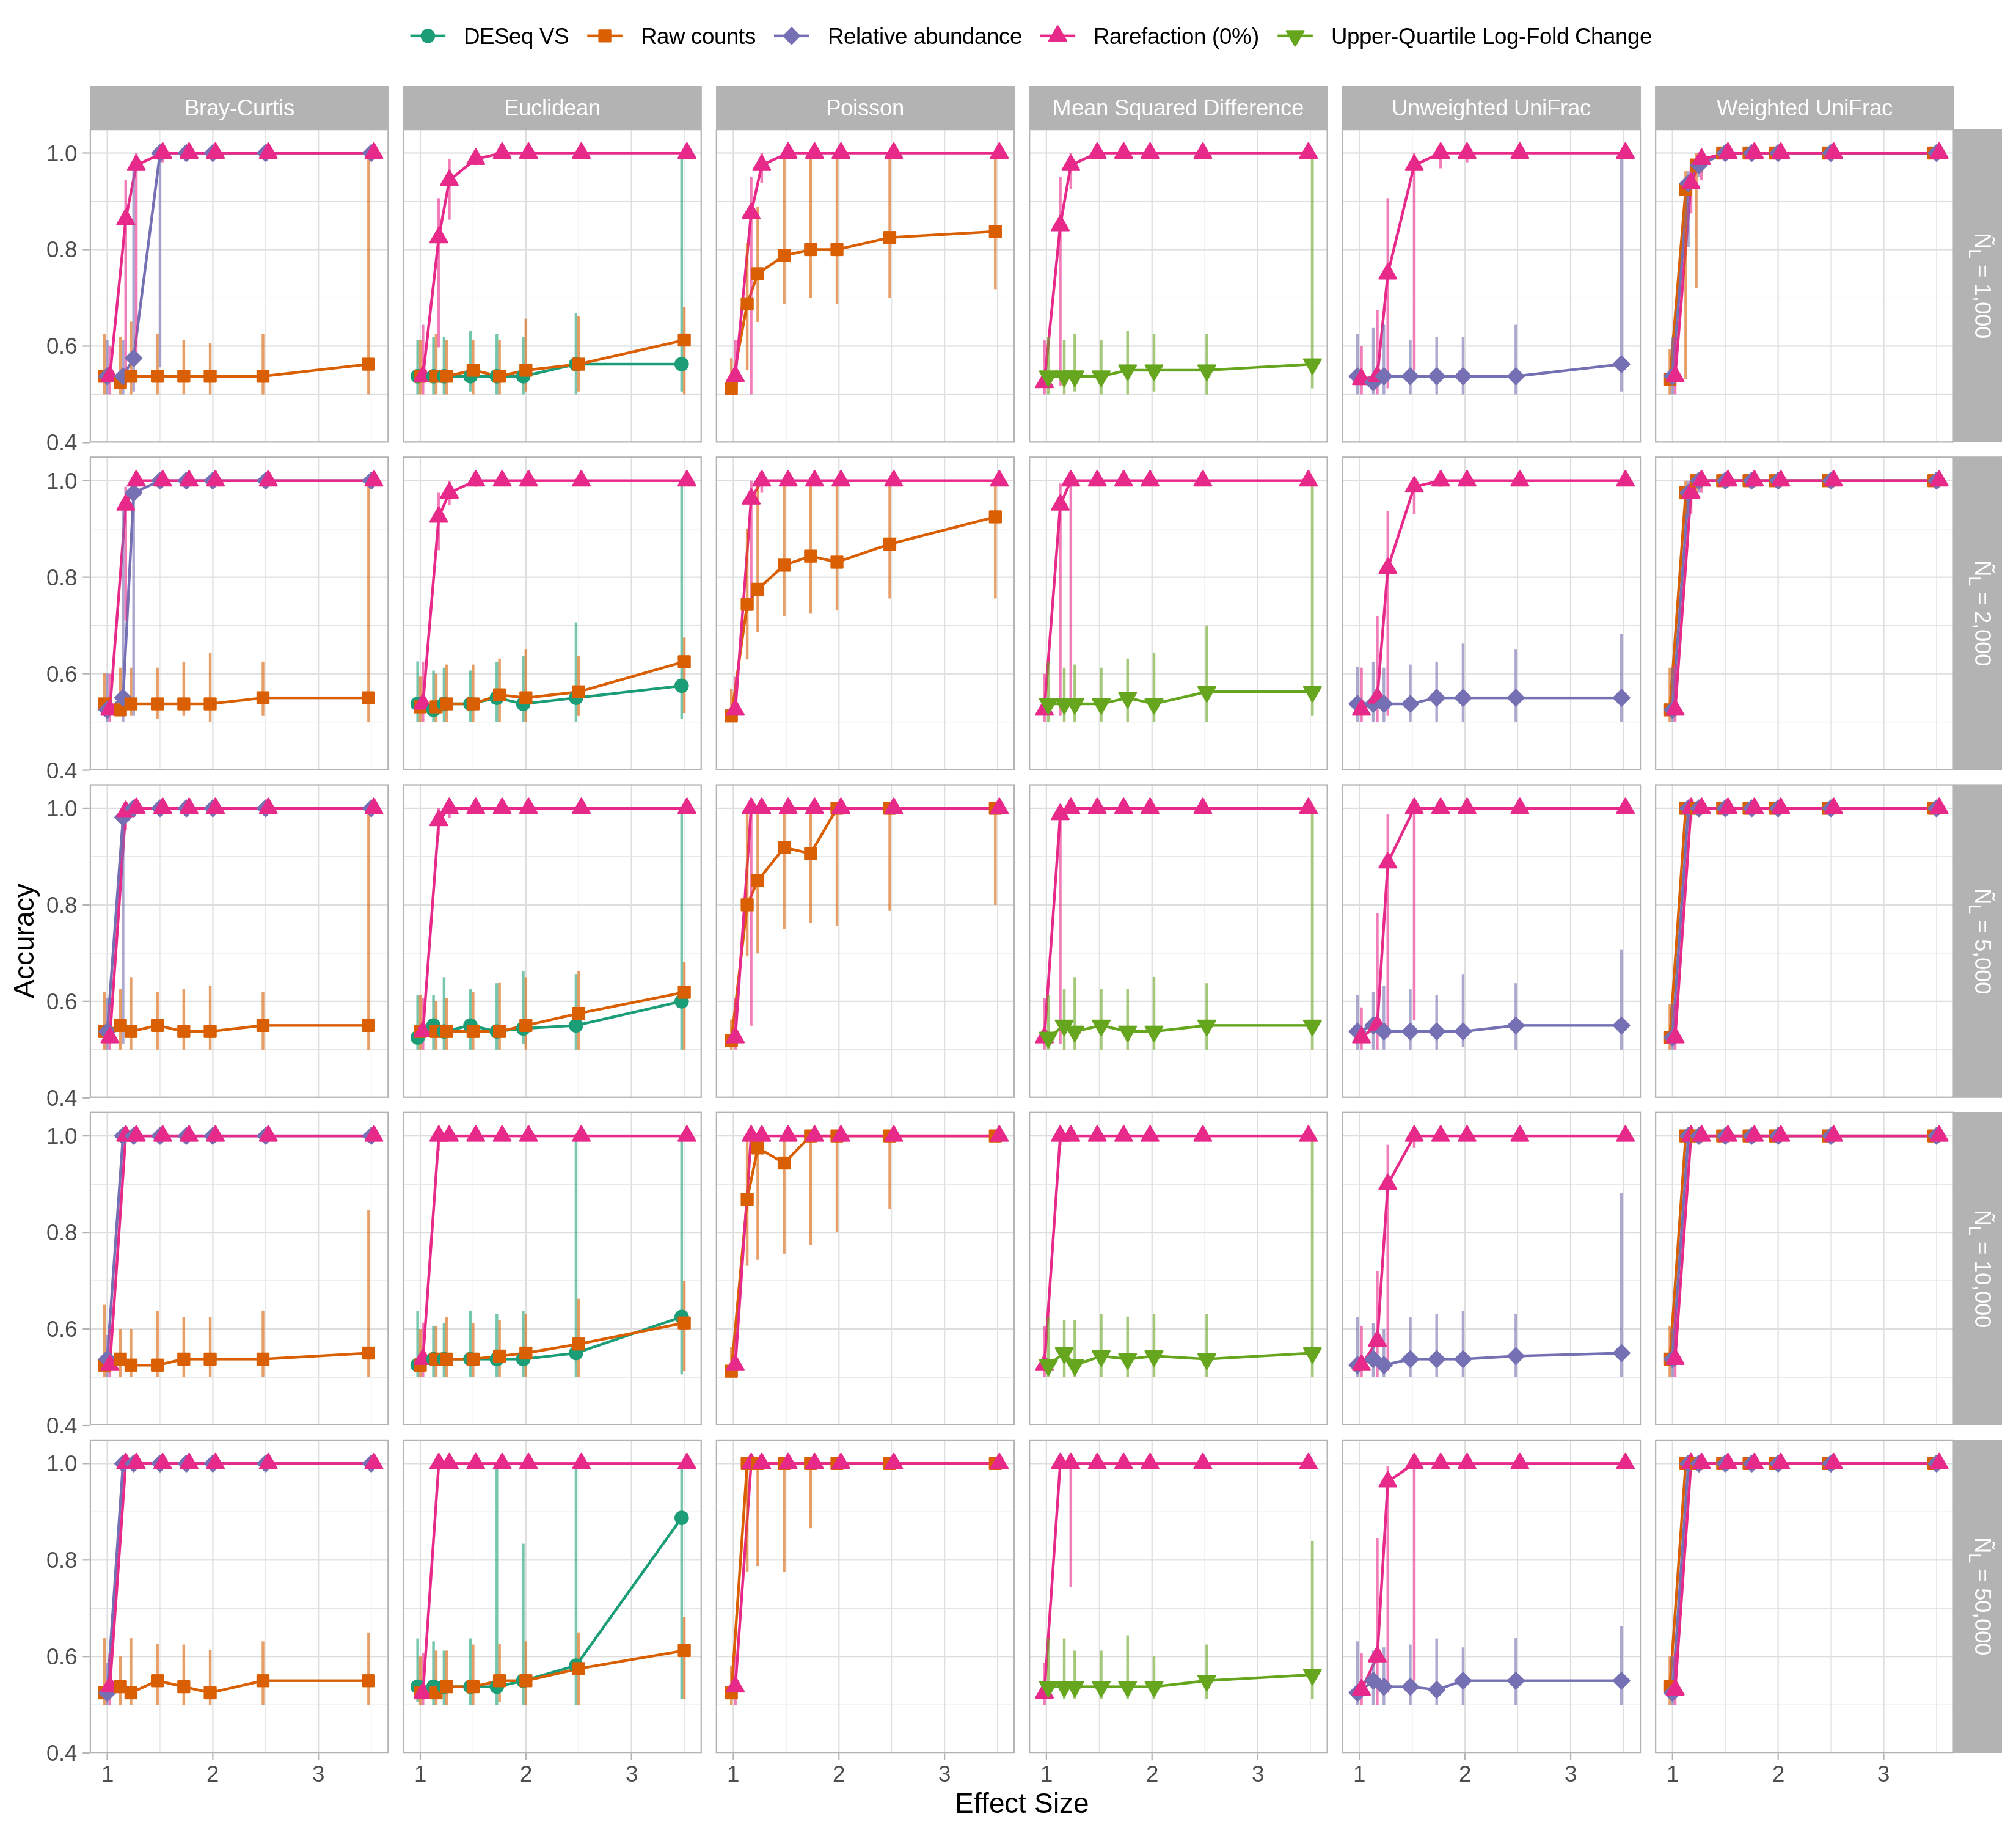
\includegraphics{figure_11.png}

\textbf{Figure 11. Clustering accuracies that used rarefaction were as
good or better than the other normalization procedures when a log-scaled
distribution of sequencing depths.} This figure is analogous to Figure 9
except that the sequencing depths for each of the 80 samples in each
simulation were drawn without replacement from a log-scaled distribution
rather than from the GlobalPatterns sequencing depths.

\newpage

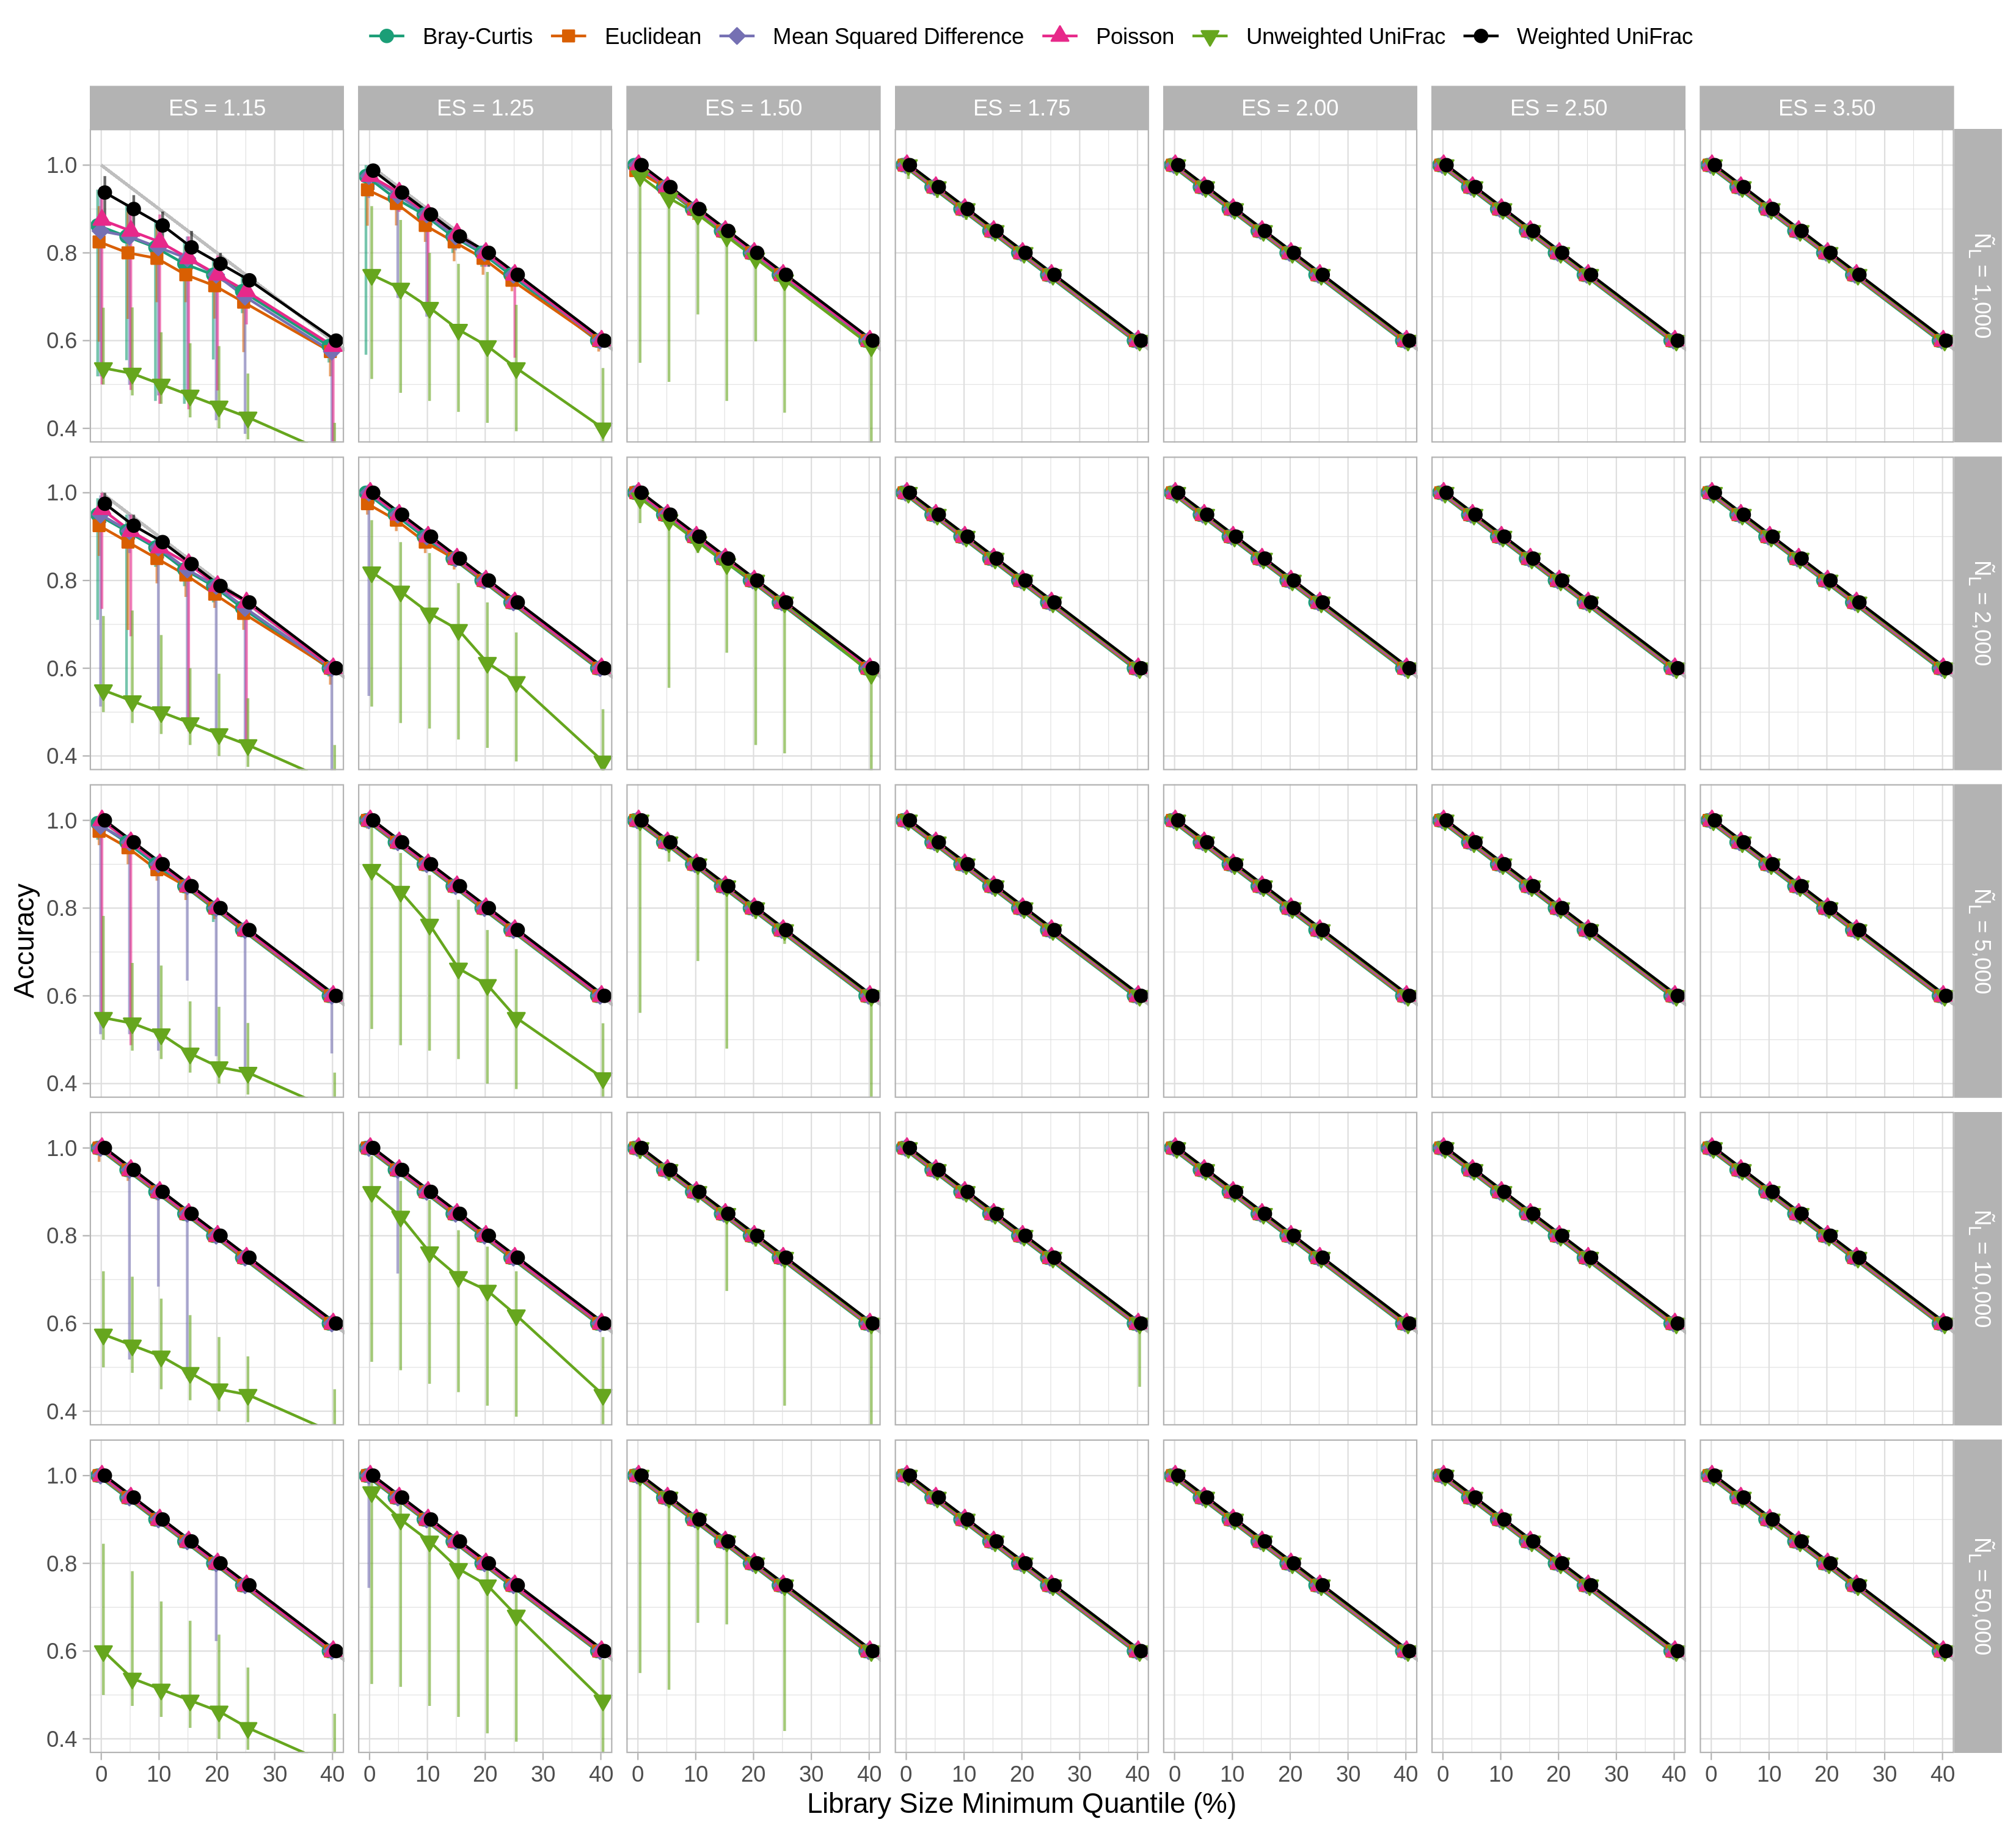
\includegraphics{figure_12.png}

\textbf{Figure 12. Rarefaction with all samples yielded clustering
accuracies that were as good or better than removing the smallest 15\%
of samples across distance calculation methods.} This figure is
analogous to Figure 8 except that the sequencing depths for each of the
80 samples in each simulation were drawn without replacement from a
log-scaled distribution rather than from the GlobalPatterns sequencing
depths.

\newpage

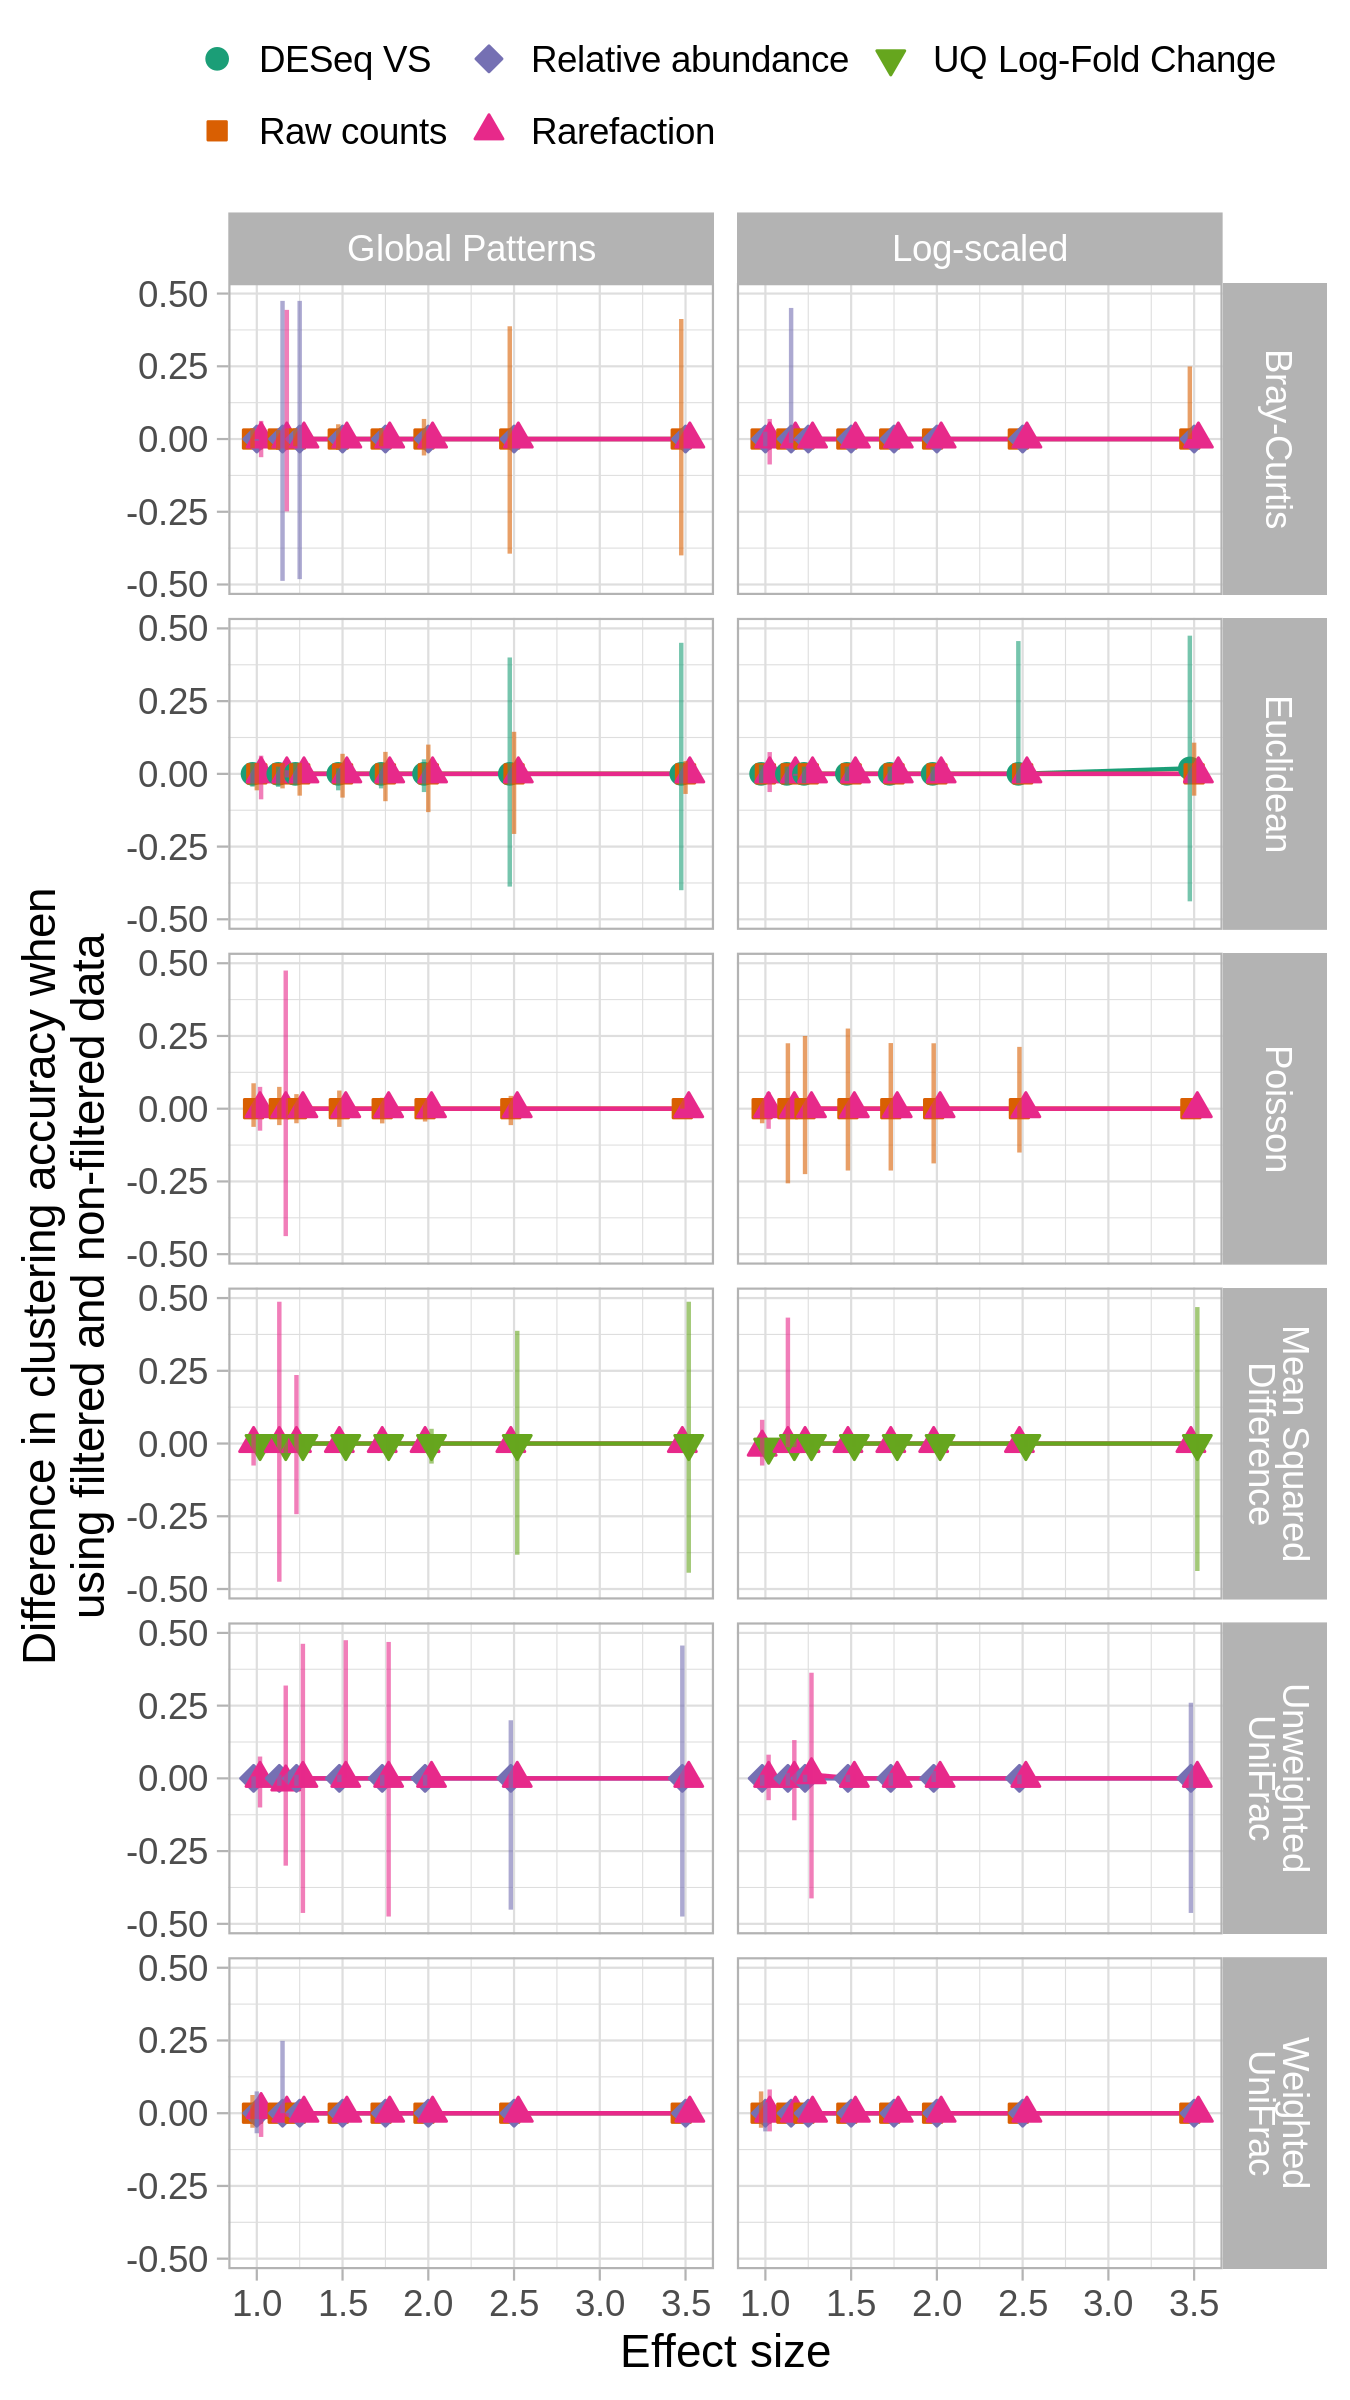
\includegraphics{figure_13.png}

\textbf{Figure 13. Normalization and distance calculation methods vary
in their sensitivity to removal of rare OTUs.} Larger values indicate
that the clustering accuracy from filtered datastets were larger than
those from non-filtered datasets. The median of 100 randomizations did
not meaningfully vary from 0.0, but the observed 95\% confidence
interval varied considerably. Data are shown for a median samling depth
(Ñ\textsubscript{L}) of 10,000 sequences when individual sequencing
depths were sampled with replacement from the GlobalPatterns dataset or
without replacement from the log-scaled distribution.

\newpage

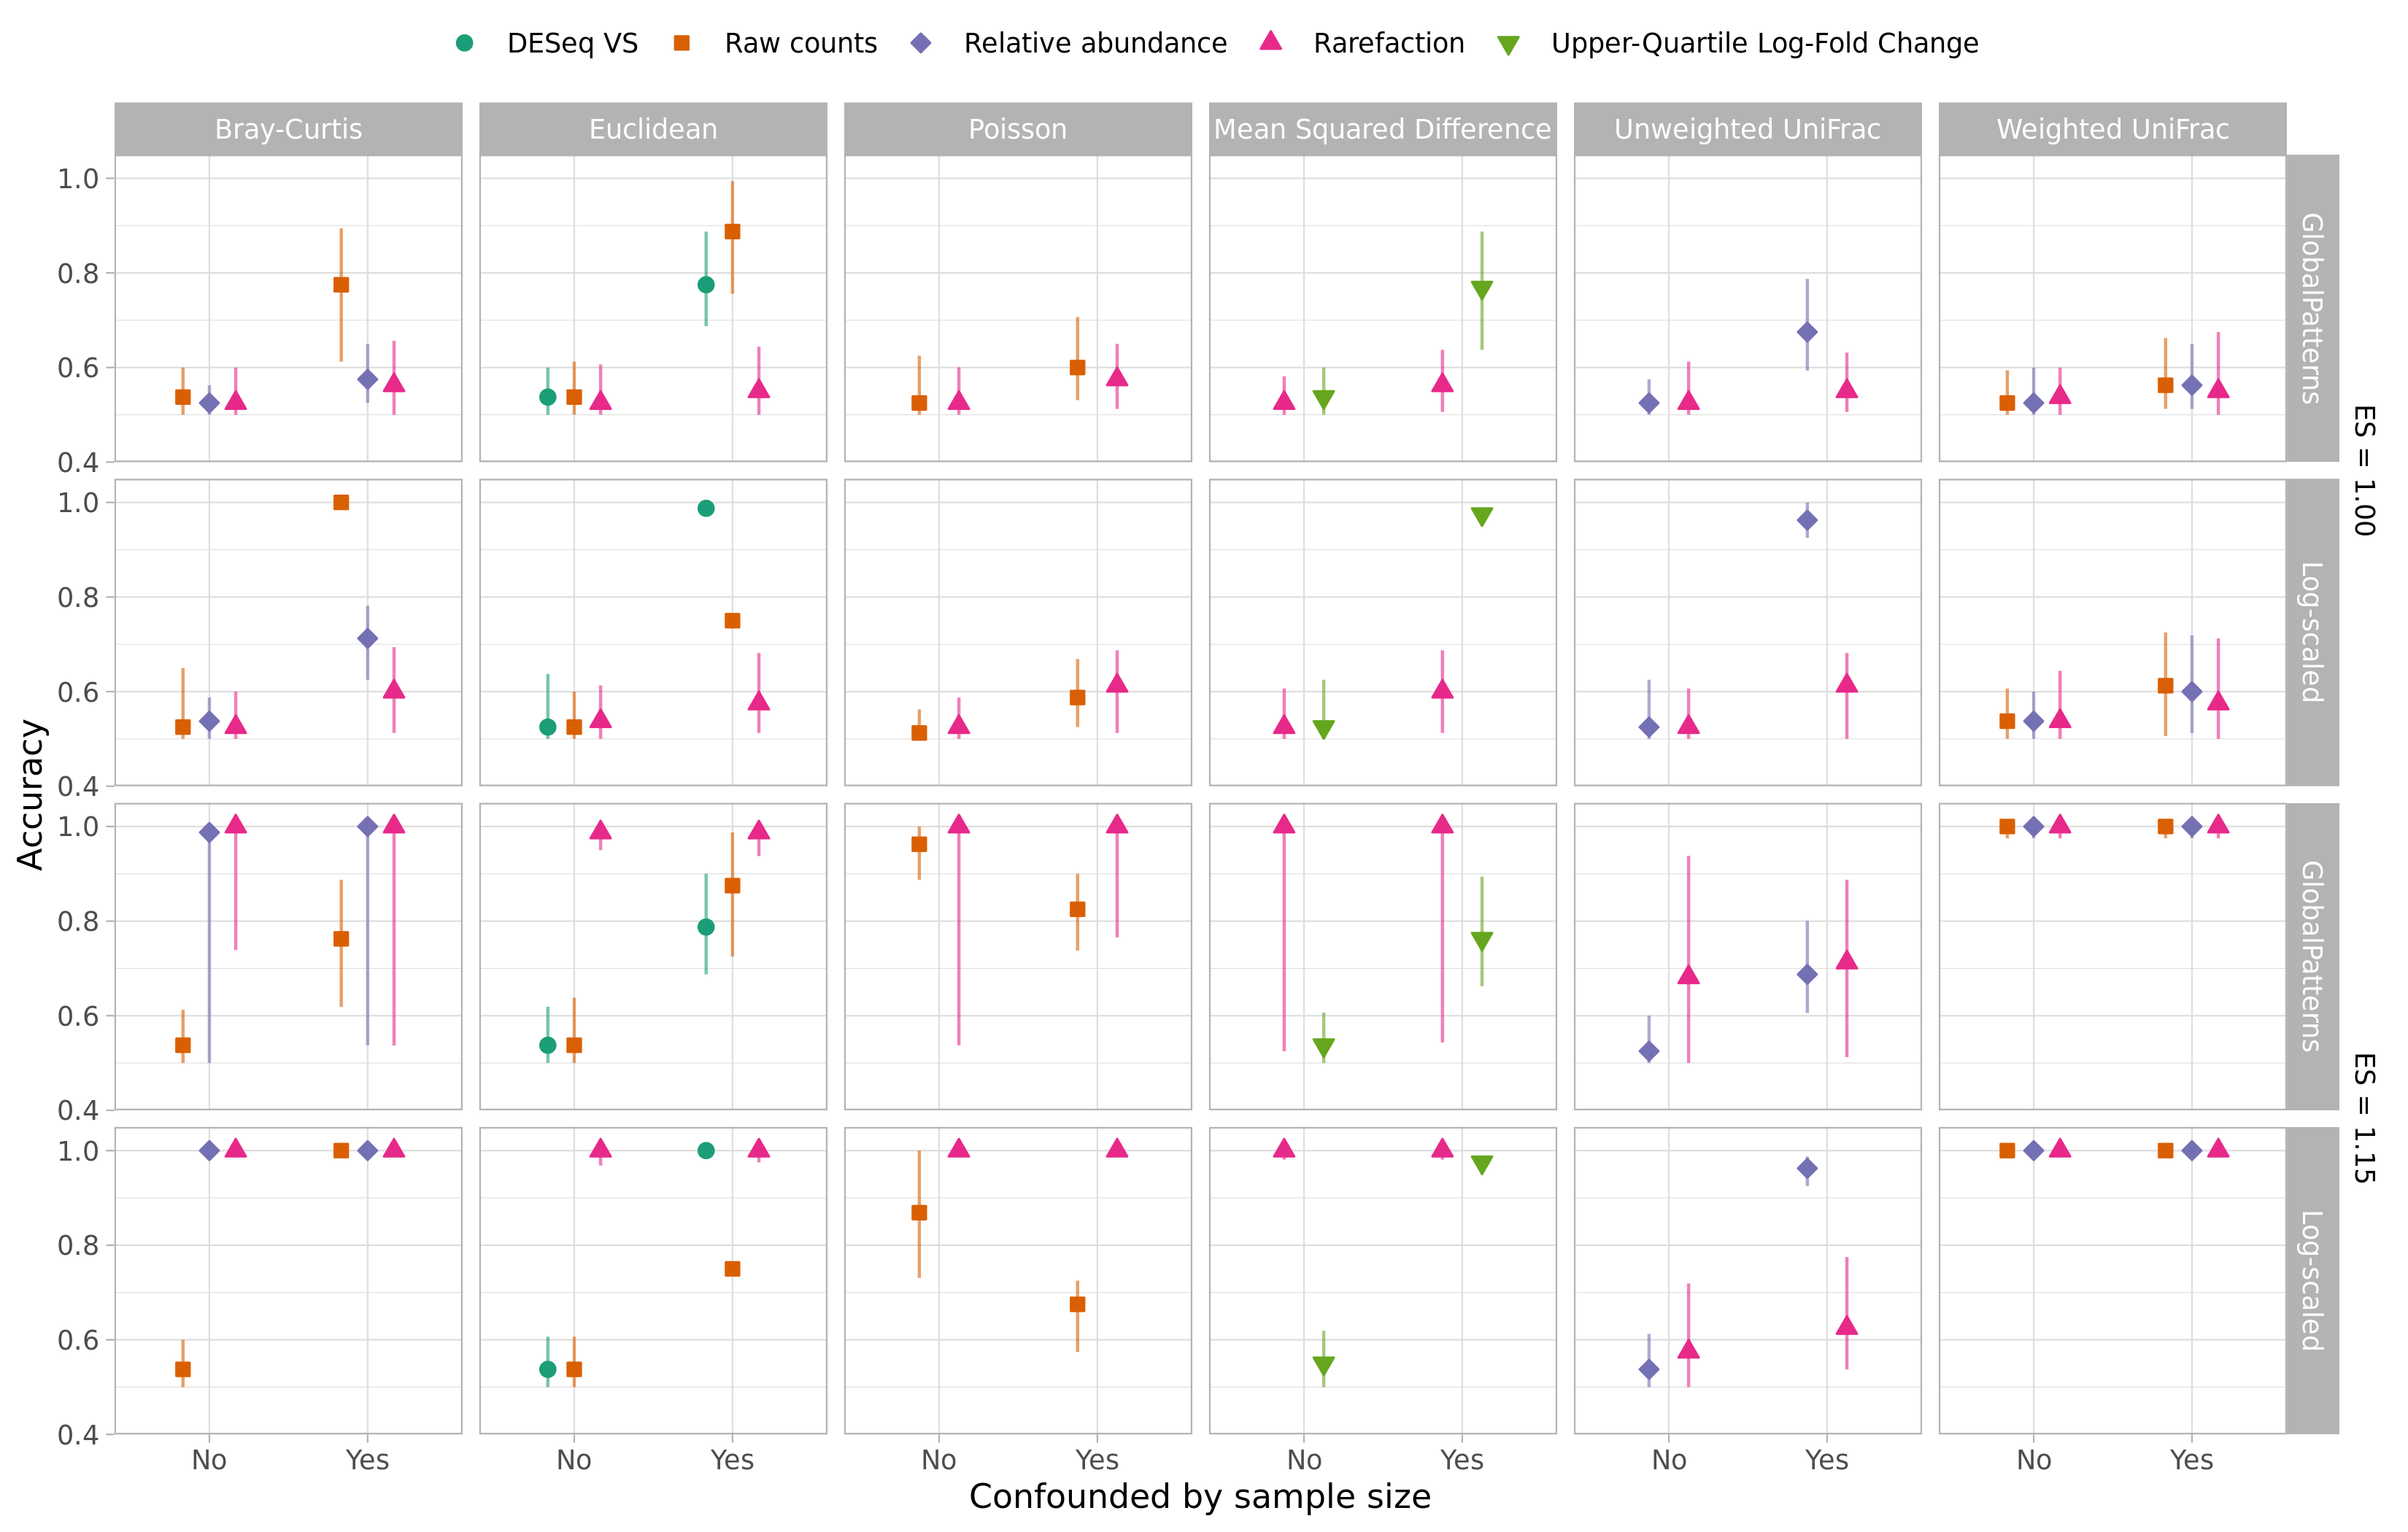
\includegraphics{figure_14.png}

\textbf{Figure 14. Rarefaction was consistently as good or better than
all other normalization methods at assigning samples to the correct
treatment group regardless of whether sequencing depth was confounded by
treatment group.} Because the clustering algorithms forced samples into
one of two groups, the exepected accuracy with an effect size of 1.00
was 0.51. With an effect size of 1.15, the expected accuracy was 1.00.
Each point represents the median of 100 replicates and the error bars
represent the observed 95\% confidence interval. Data are shown for a
median samling depth (Ñ\textsubscript{L}) of 10,000 sequences when
individual sequencing depths were sampled with replacement from the
GlobalPatterns dataset or without replacement from the log-scaled
distribution.

\newpage

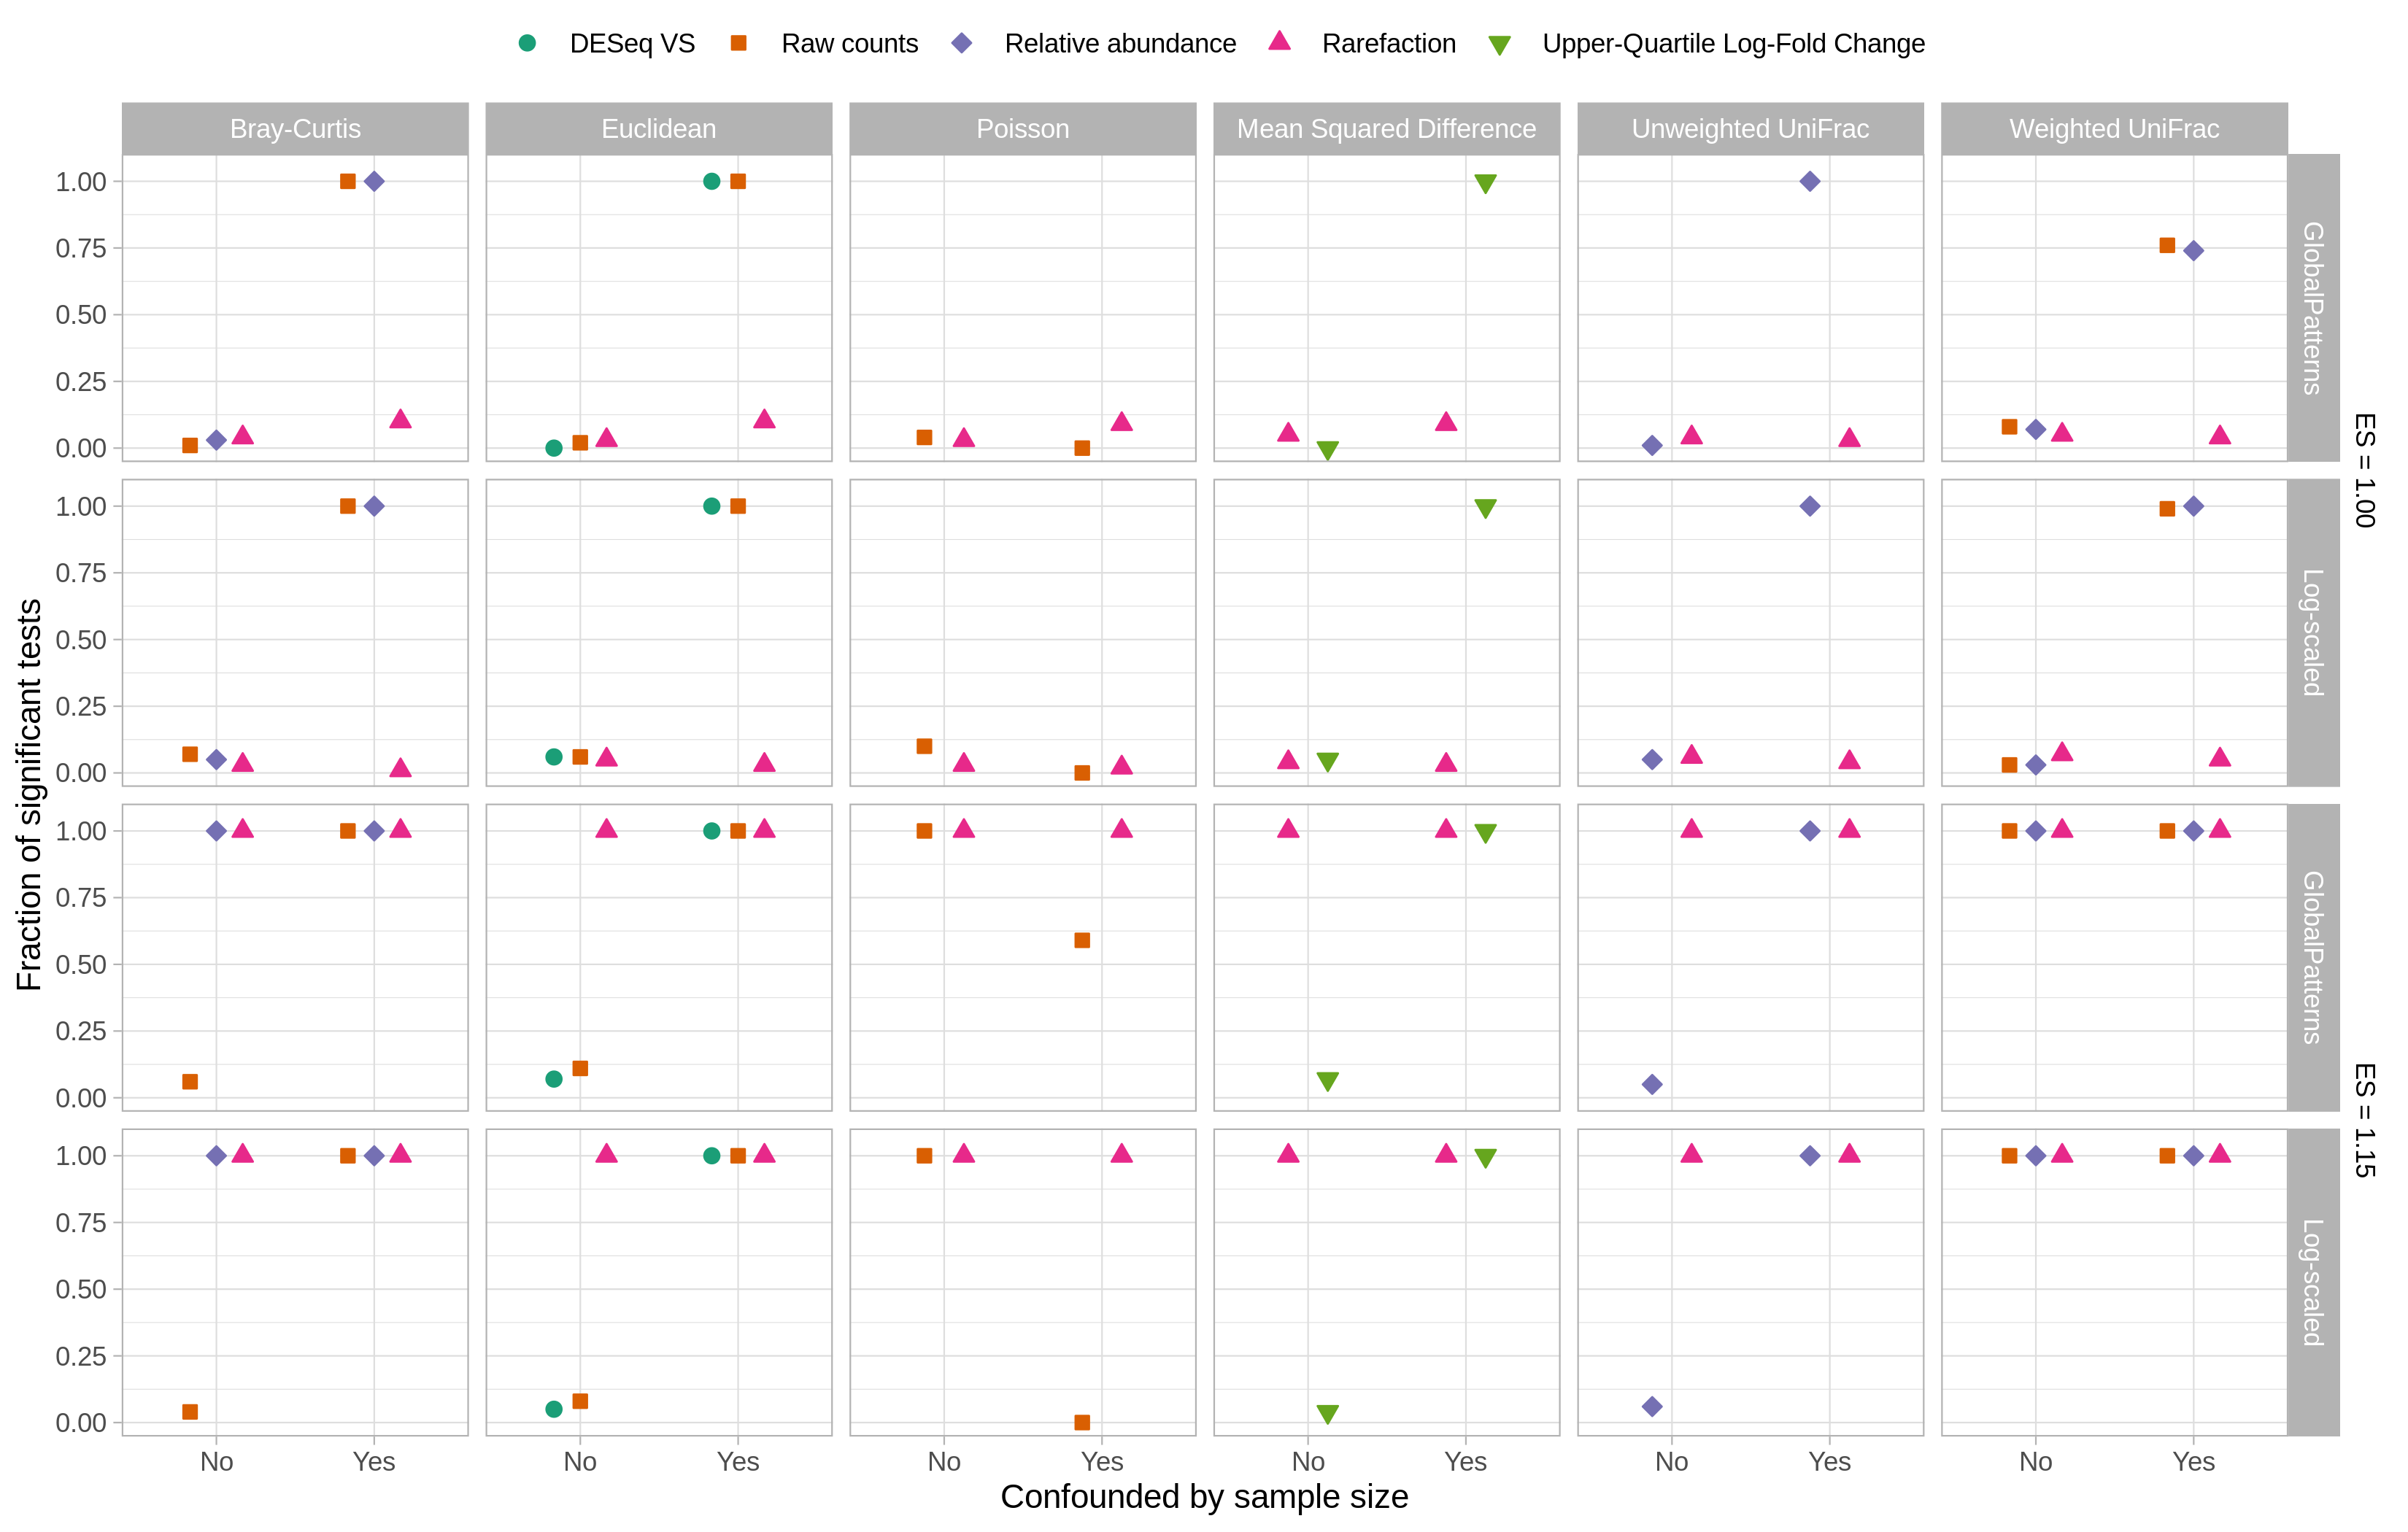
\includegraphics{figure_15.png}

\textbf{Figure 15. Rarefaction was consistently as good or better than
all other normalization methods at controlling for Type I error and
maximizing power to detect differences in treatment group using adonis2
regardless of whether sequencing depth was confounded by treatment
group.} Type I errors were assessed as the fraction of 100 simulations
that yielded a significant P-value (i.e., less than or equal to 0.05) at
an effect size of 1.00. Power was assesed as the fraction of 100
simulations that yieleded a significant P-Value at an effect size of
1.15. Data are shown for a median samling depth (Ñ\textsubscript{L}) of
10,000 sequences when individual sequencing depths were sampled with
replacement from the GlobalPatterns dataset or without replacement from
the log-scaled distribution.

\newpage

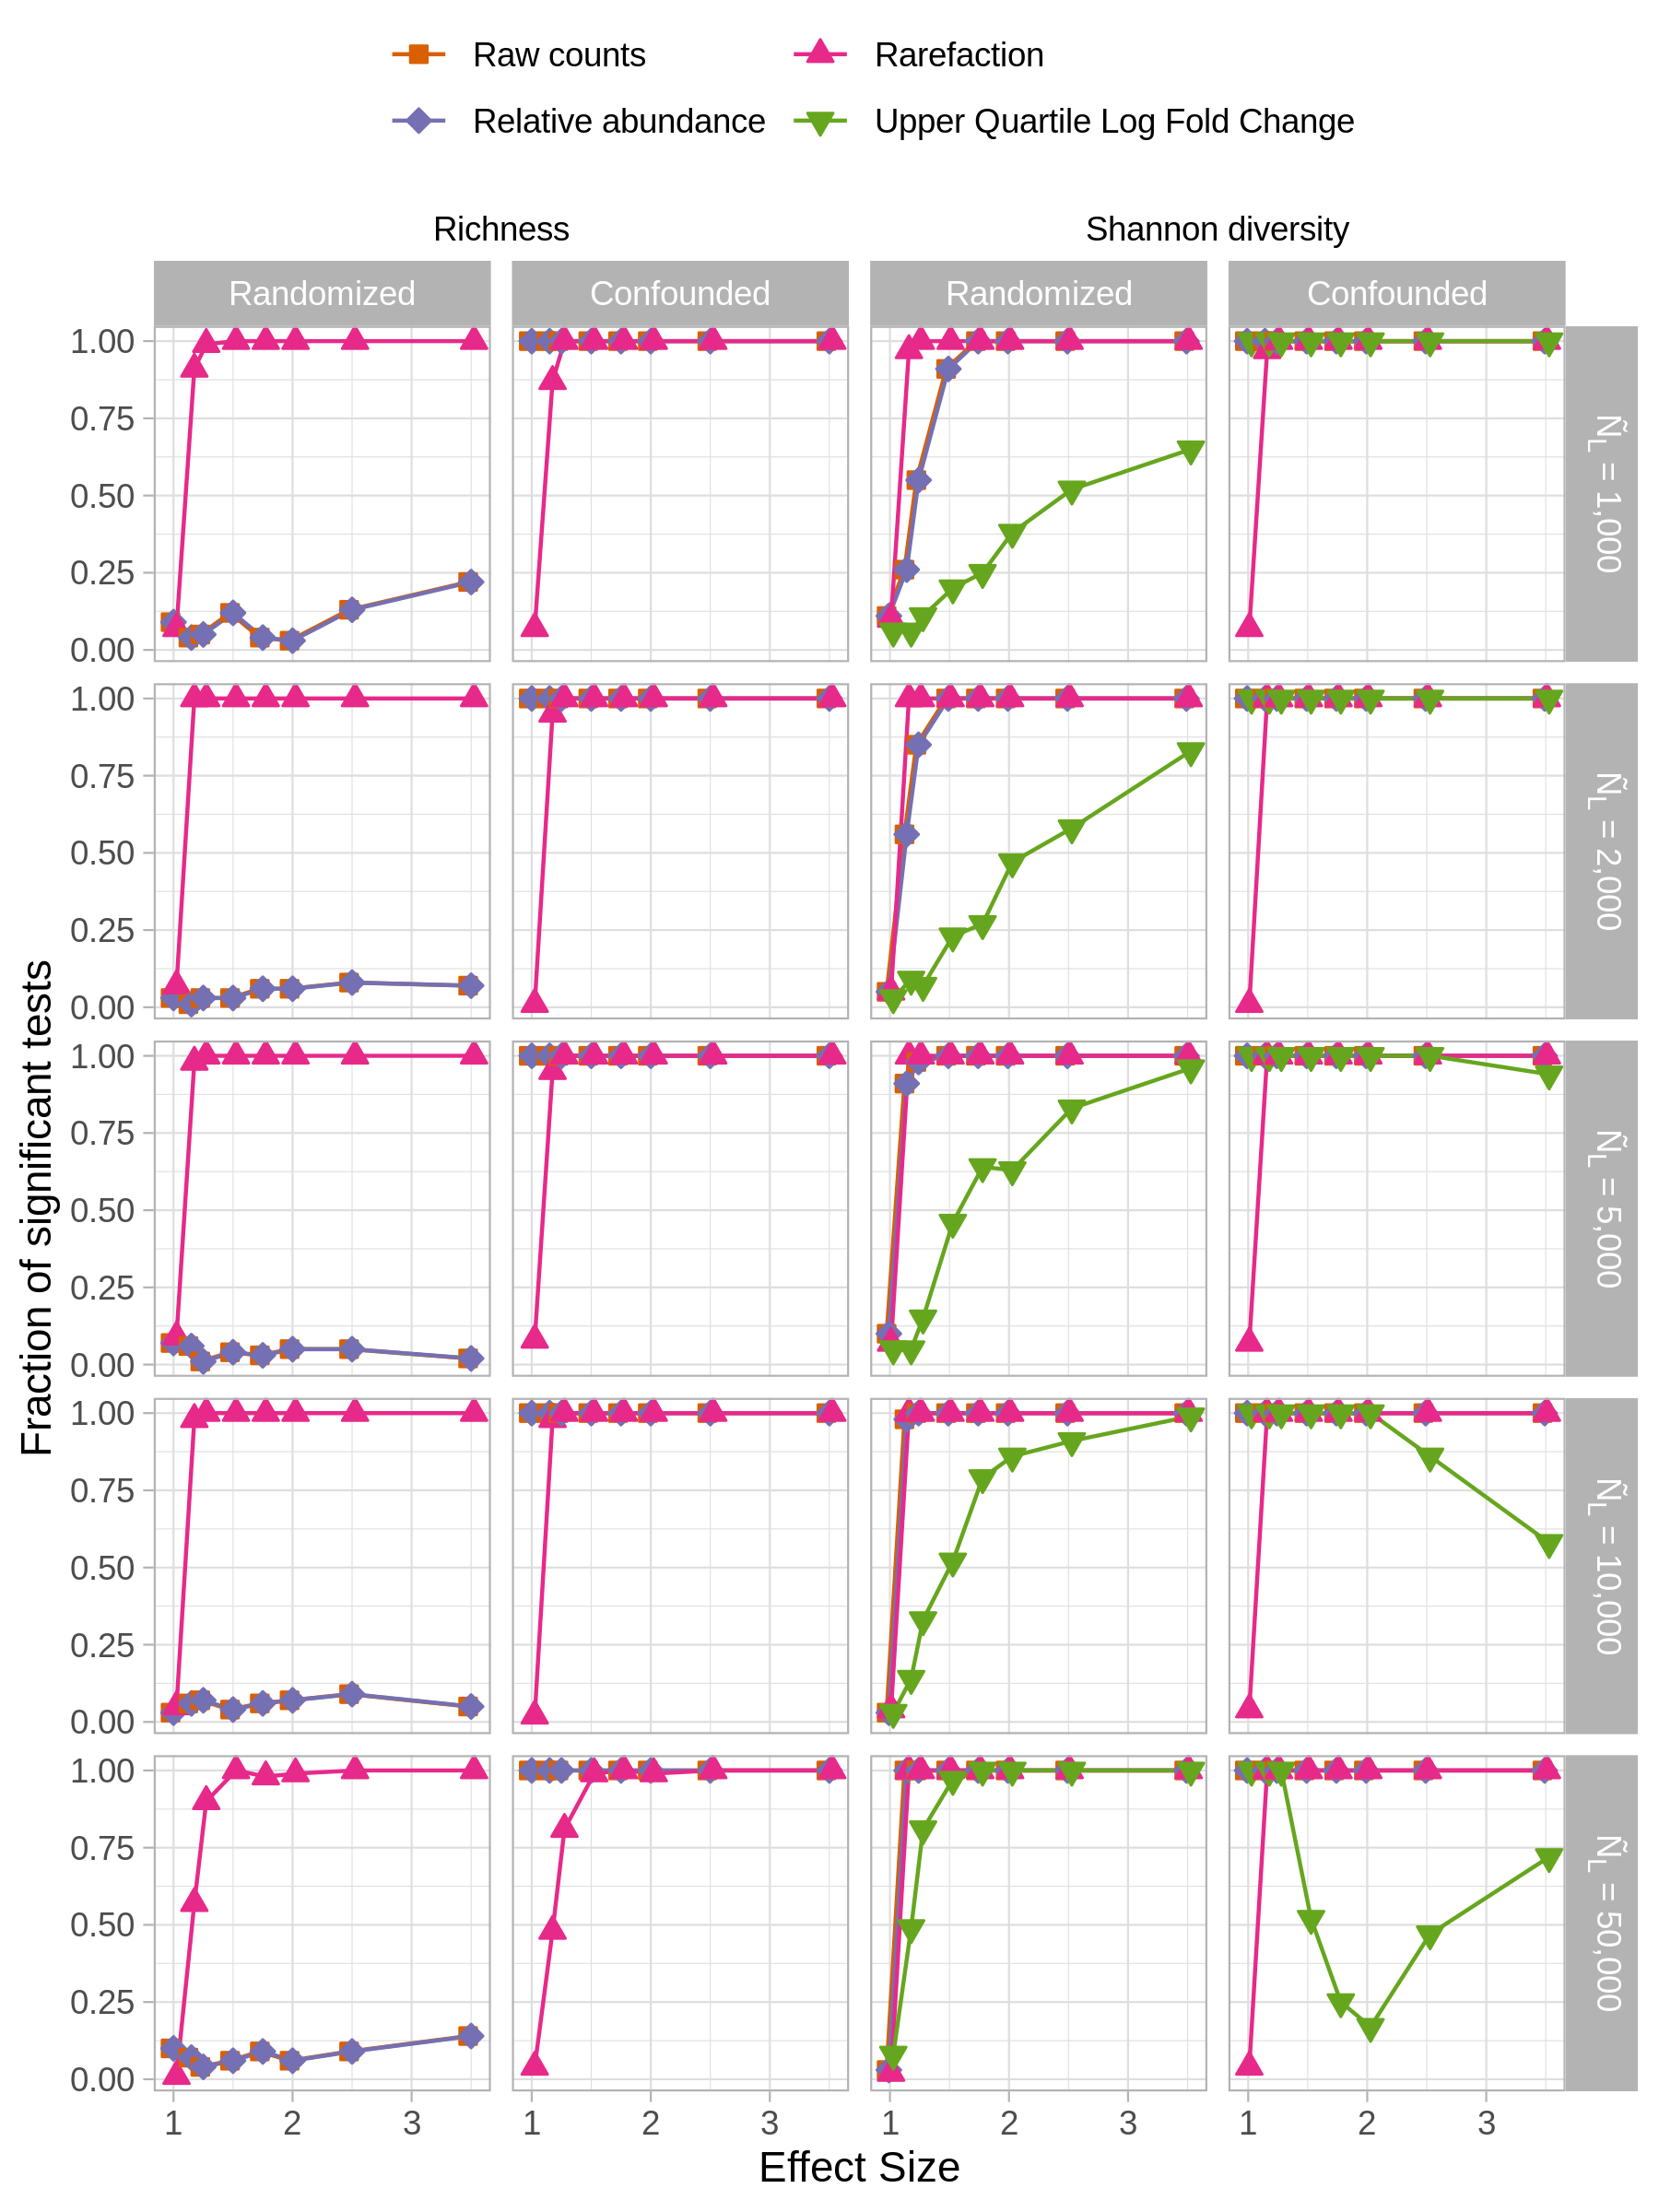
\includegraphics{figure_16.png}

\textbf{Figure 16. Rarefaction was consistently as good or better than
all other normalization methods at controlling for Type I error and
maximizing power to detect differences in treatment group using
alpha-diversity metrics regardless of whether sequencing depth was
confounded by treatment group.} Statistical comparisons of OTU richness
and Shannon diversity were performed using the non-parametric Wilcoxon
two-sampled test. Type I errors were assessed as the fraction of 100
simulations that yielded a significant P-value (i.e., less than or equal
to 0.05) at an effect size of 1.00. Power was assesed as the fraction of
100 simulations that yieleded a significant P-Value at an effect size of
1.15. Data are shown for when the case when individual sequencing depths
were sampled with replacement from the GlobalPatterns dataset.

\newpage

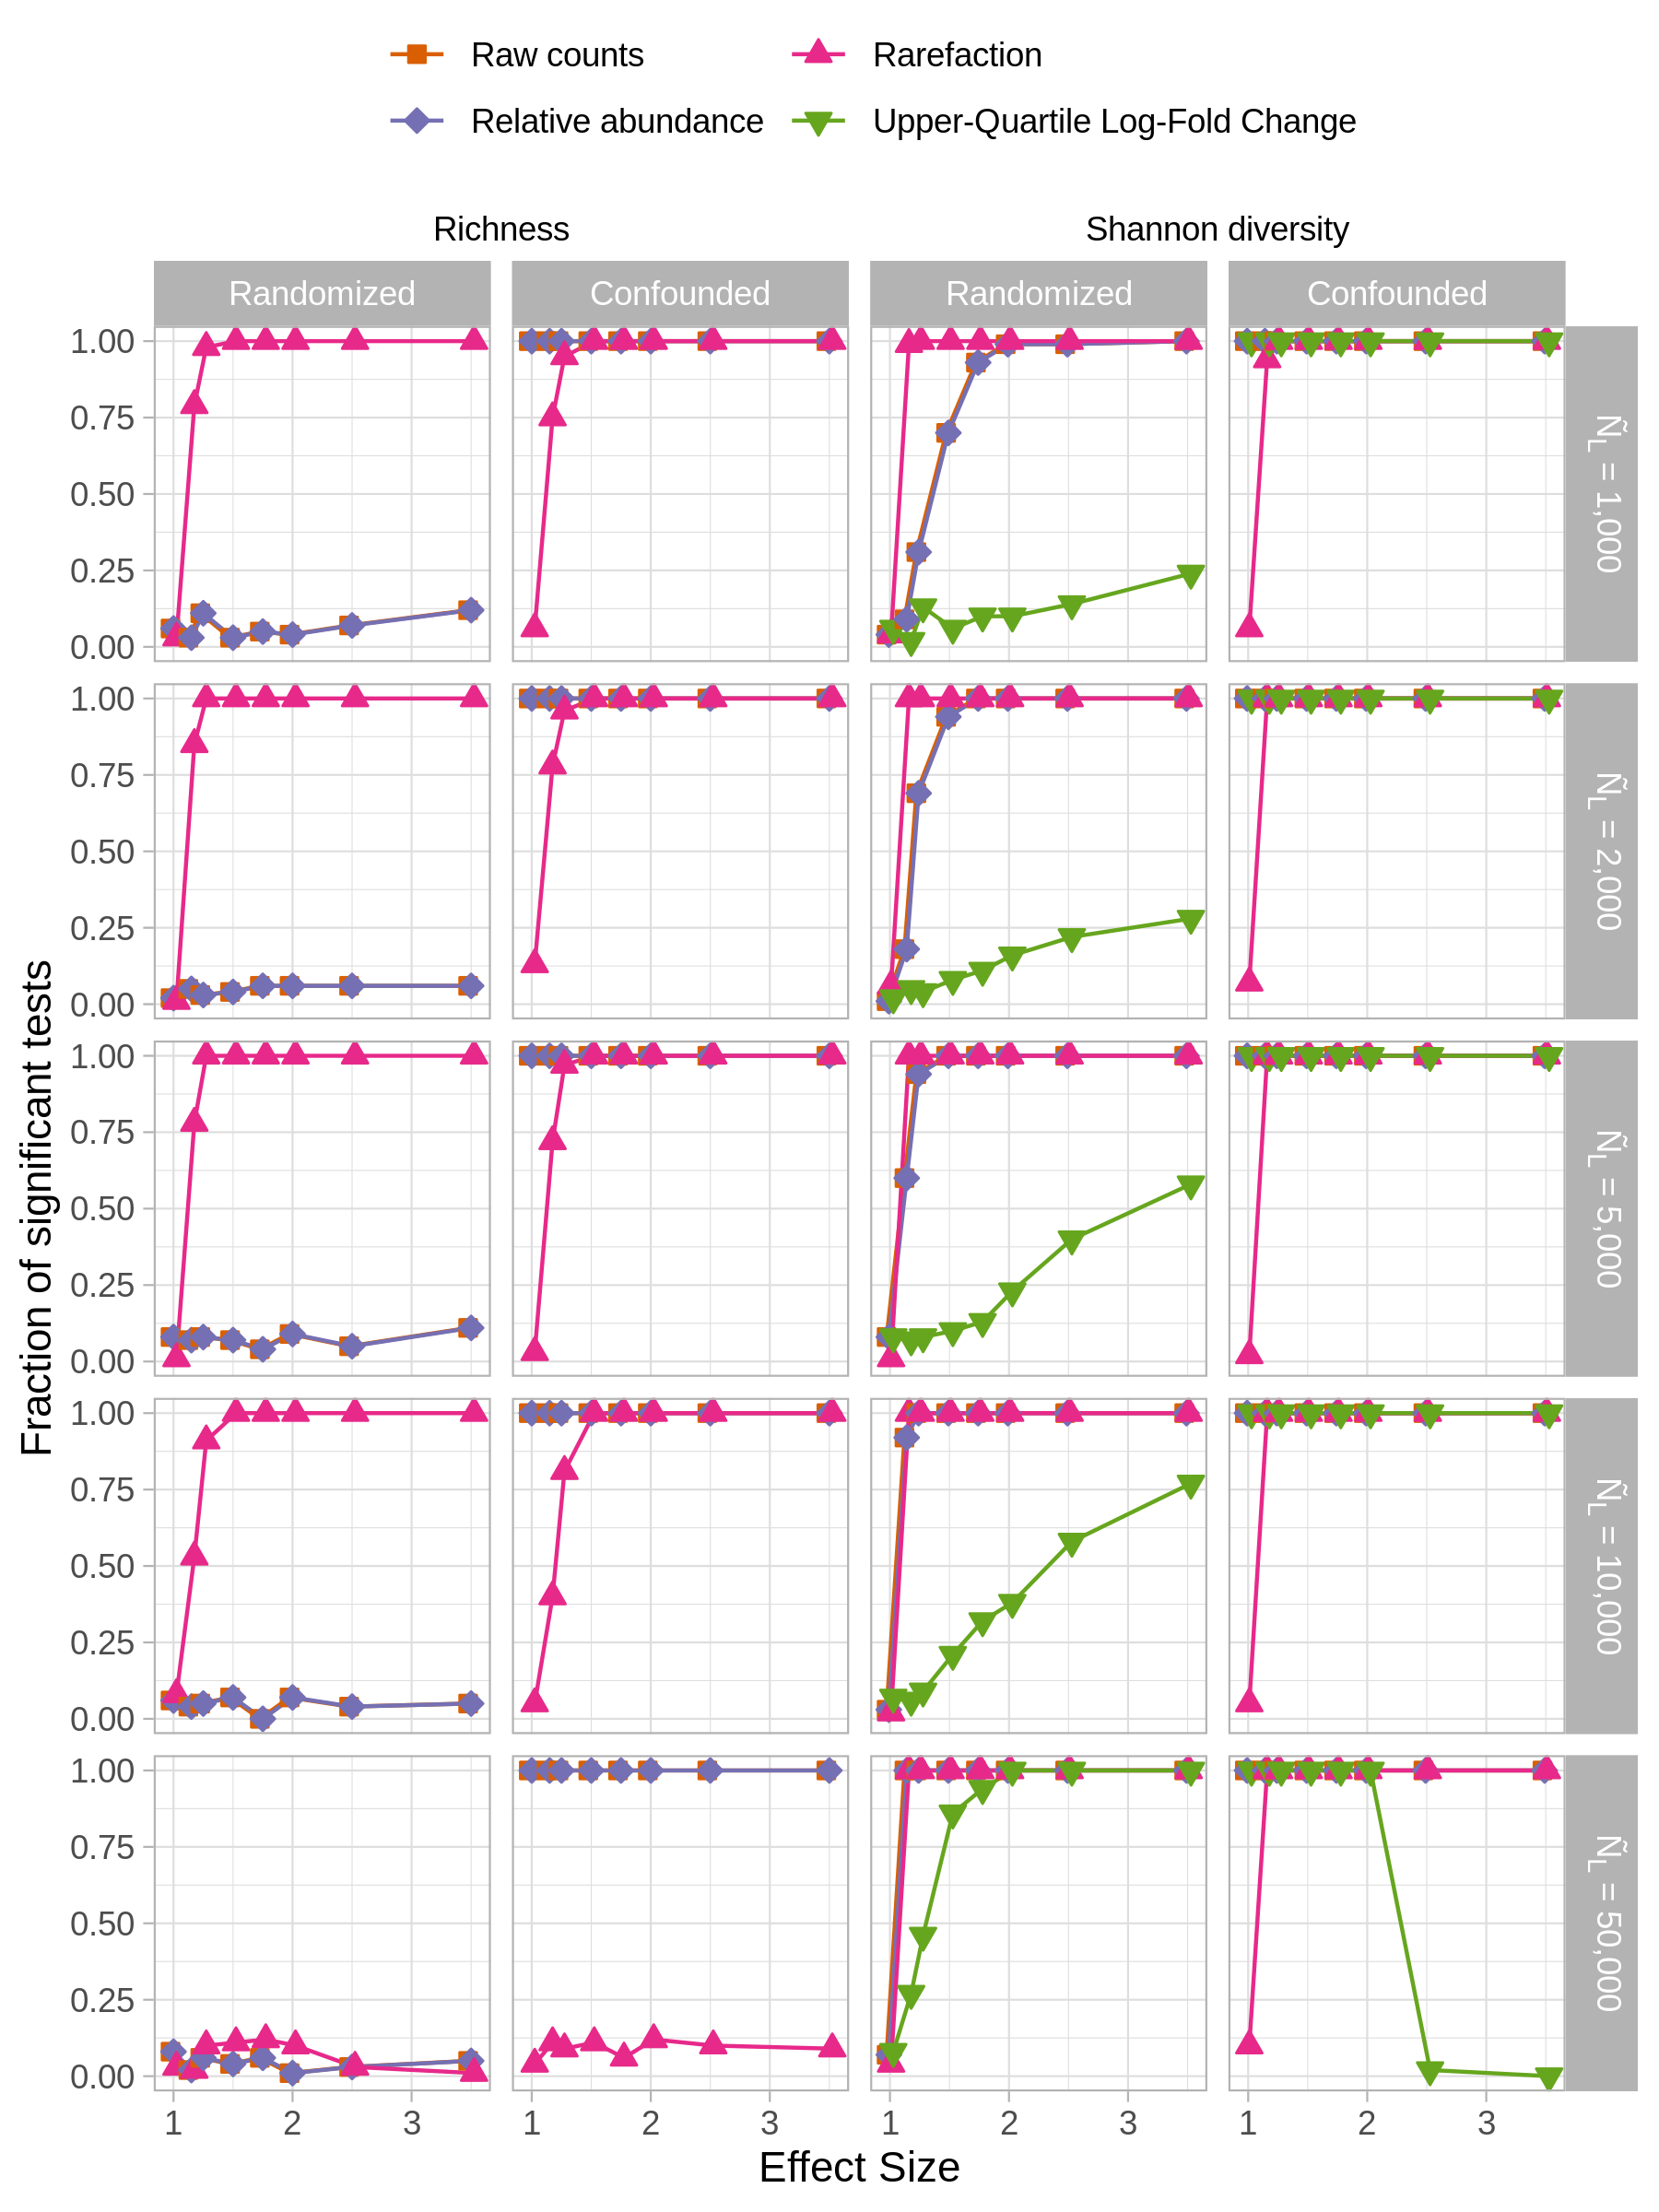
\includegraphics{figure_17.png}

\textbf{Figure 17. Rarefaction was consistently as good or better than
all other normalization methods at controlling for Type I error and
maximizing power to detect differences in treatment group using
alpha-diversity metrics regardless of whether sequencing depth was
confounded by treatment group.} Statistical comparisons of OTU richness
and Shannon diversity were performed using the non-parametric Wilcoxon
two-sampled test. Type I errors were assessed as the fraction of 100
simulations that yielded a significant P-value (i.e., less than or equal
to 0.05) at an effect size of 1.00. Power was assesed as the fraction of
100 simulations that yieleded a significant P-Value at an effect size of
1.15. Data are shown for when the case when individual sequencing depths
were sampled without replacement from the log-scaled distribution.

\end{document}
